
%------------------ LEARNING RATE 10: ------------------
\subsubsection{Learning Rate = 10}
% -- 1h, lr 10 --
\begin{figure}[H]
  \centering
  \begin{subfigure}{.5\textwidth}
    \centering
    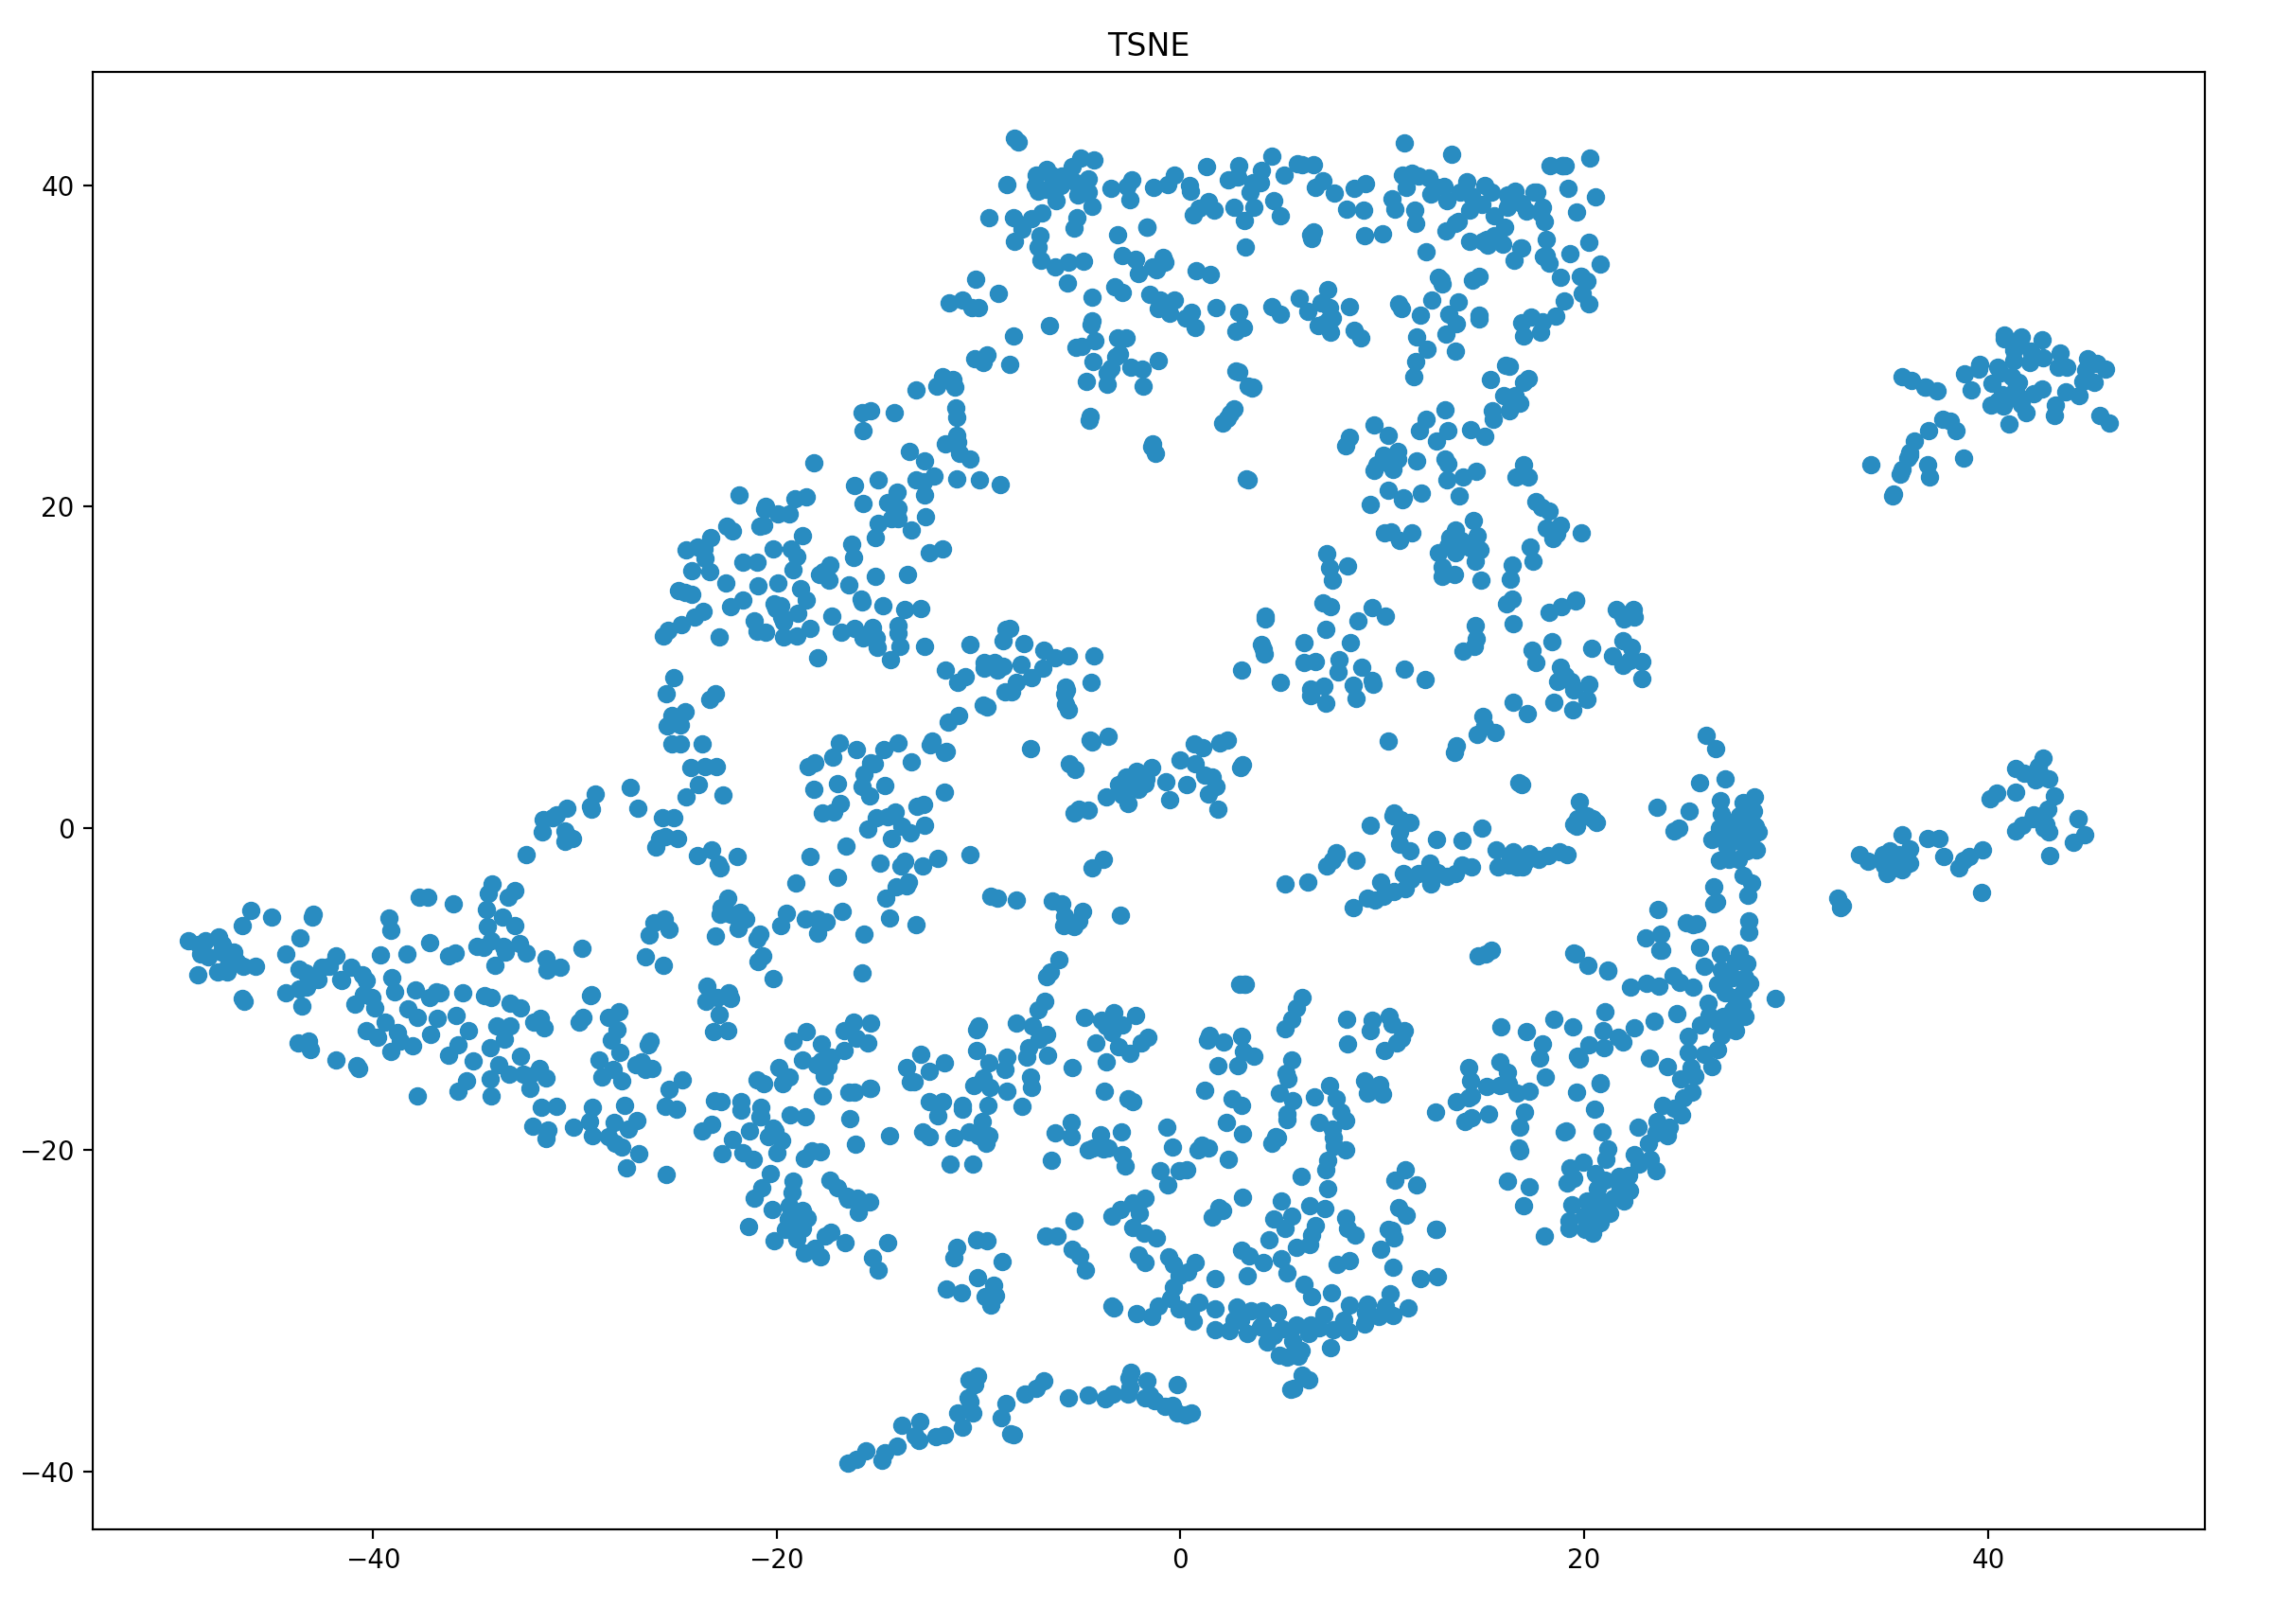
\includegraphics[width=0.9\textwidth]{./images/tsneParametersTest/learningRate/lr10-1hTSNE.png}
  \end{subfigure}%
  \begin{subfigure}{.5\textwidth}
    \centering
    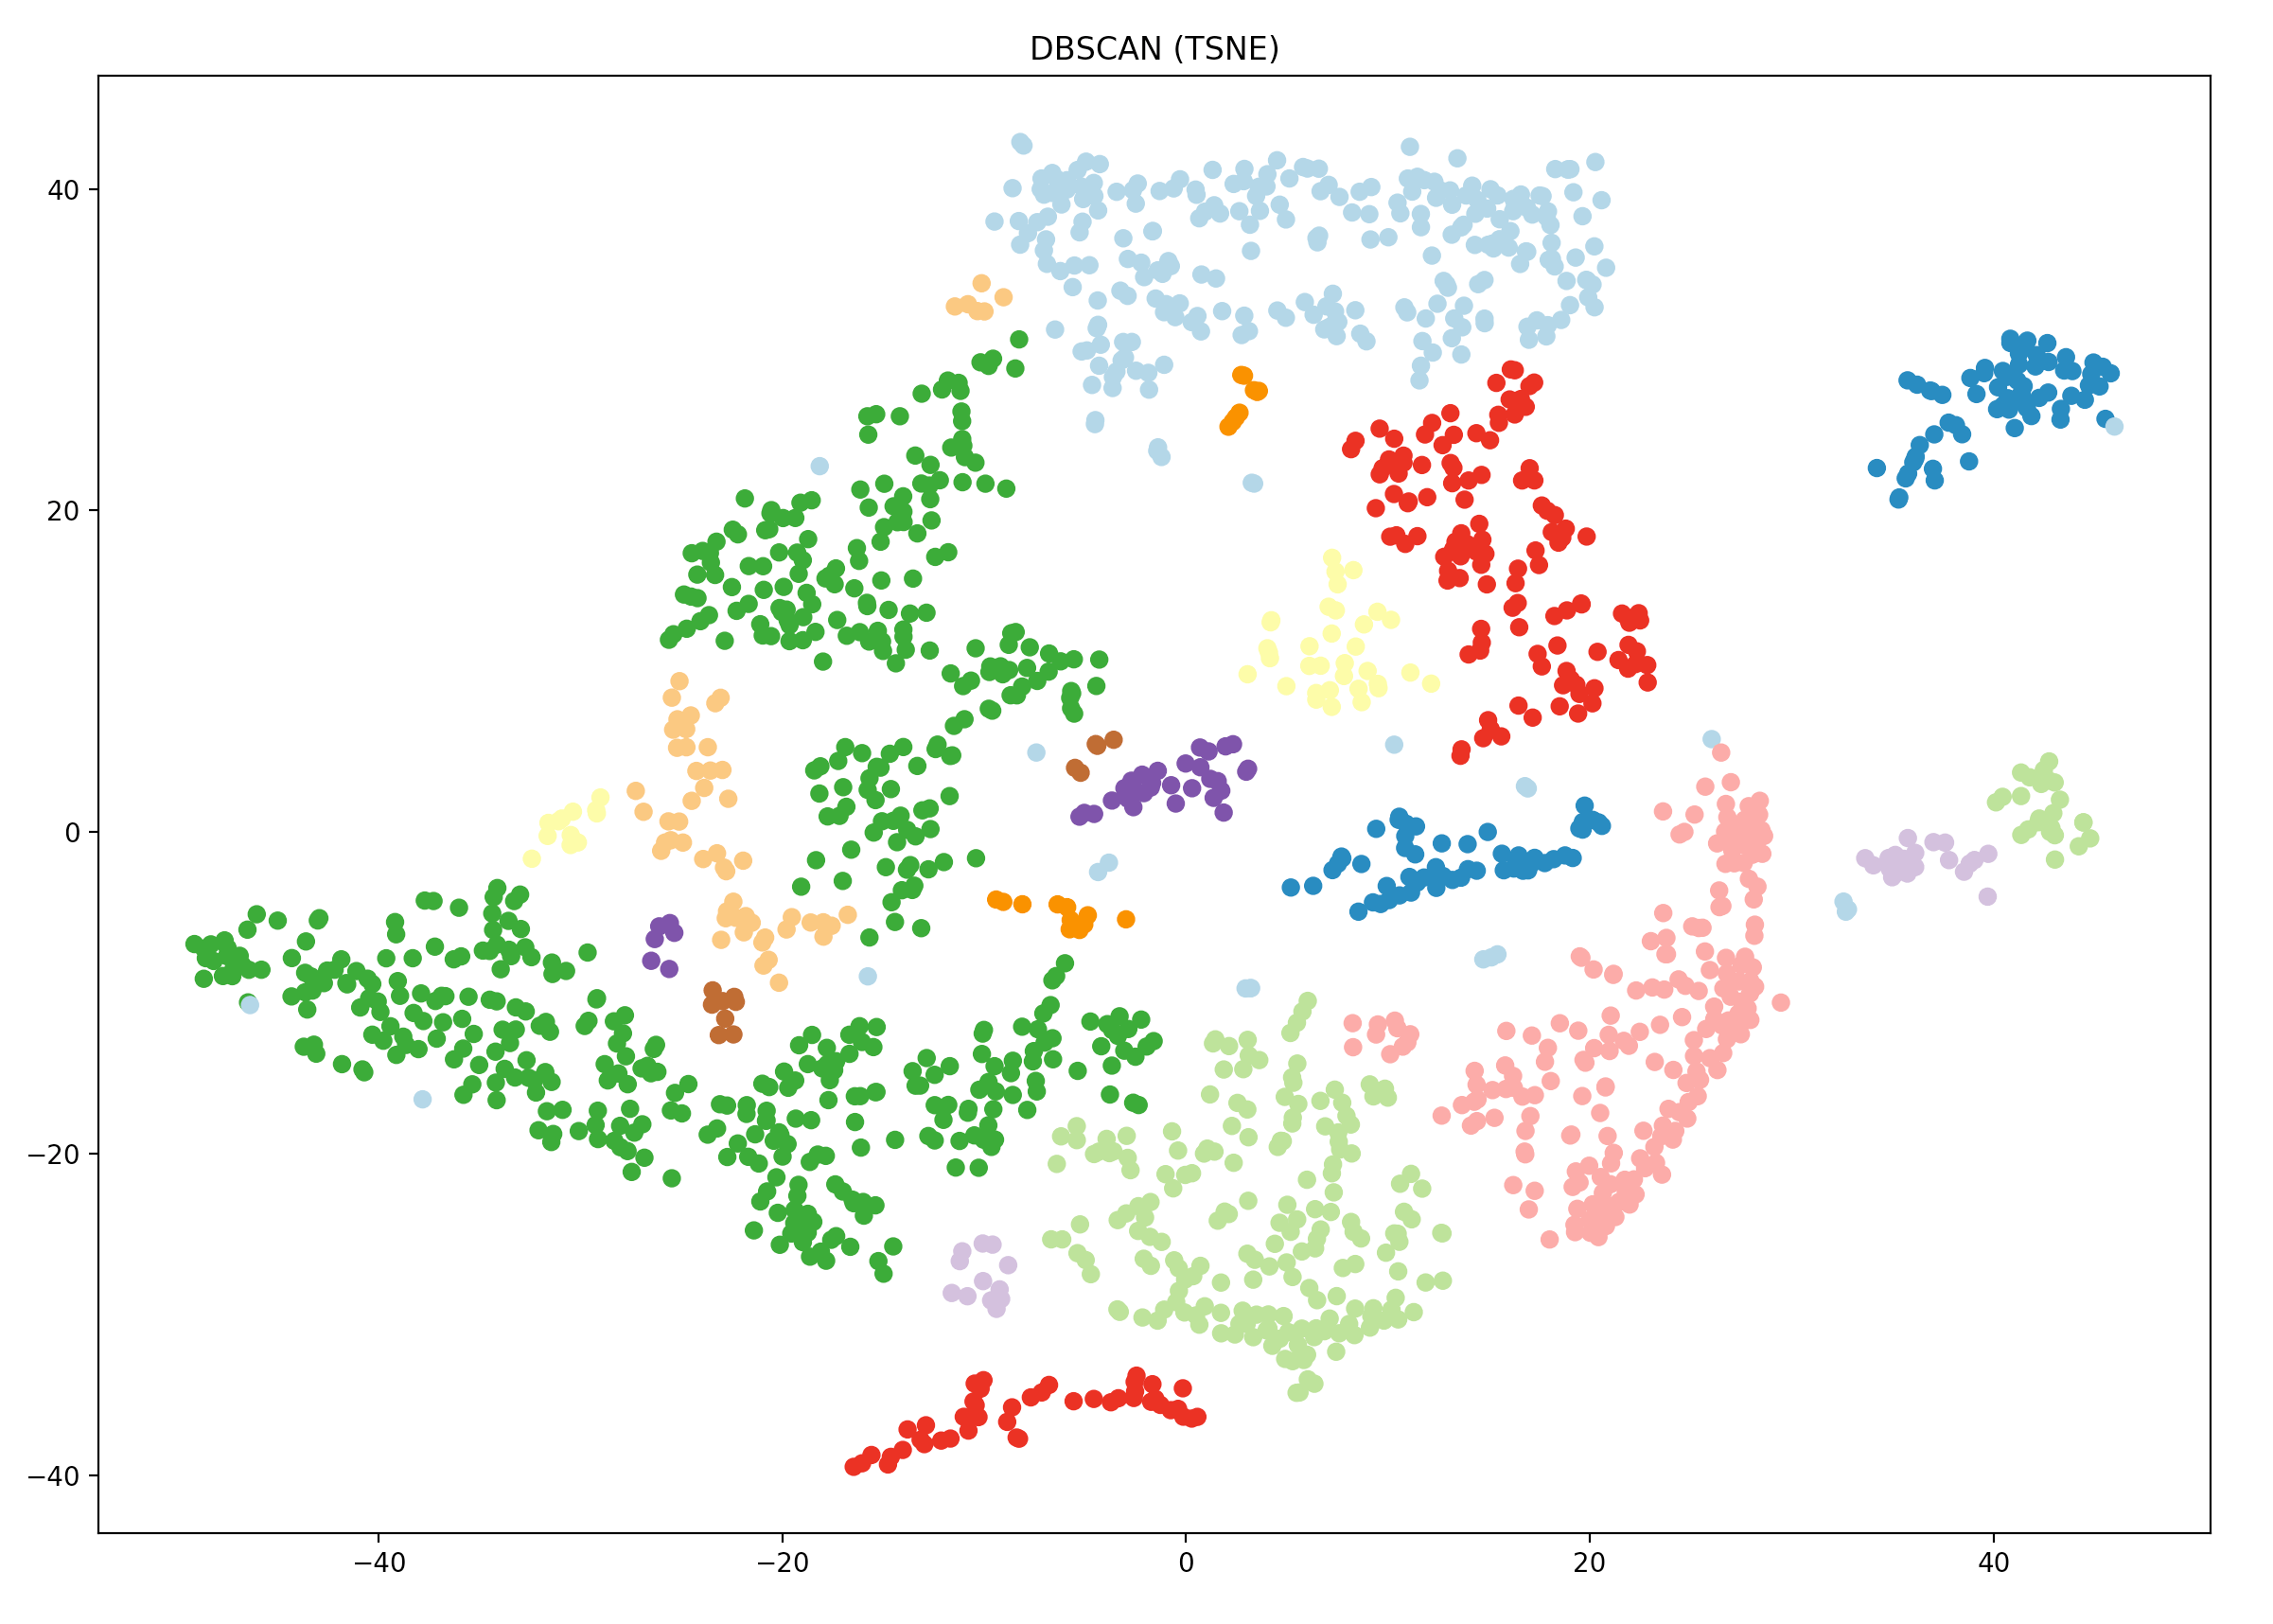
\includegraphics[width=0.9\textwidth]{./images/tsneParametersTest/learningRate/lr10-1hDBSCAN.png}
  \end{subfigure}
	\caption{\textbf{1h} data files, t-SNE calculated with the following parameters: perplexity=40, n\_iter=5000, \textbf{learning\_rate=10}}
	\label{figure:1hlr10TSNE}
\end{figure}

% -- 3h, lr 10 --
\begin{figure}[H]
	\centering
	
  \centering
	\begin{subfigure}{.5\textwidth}
    \centering
    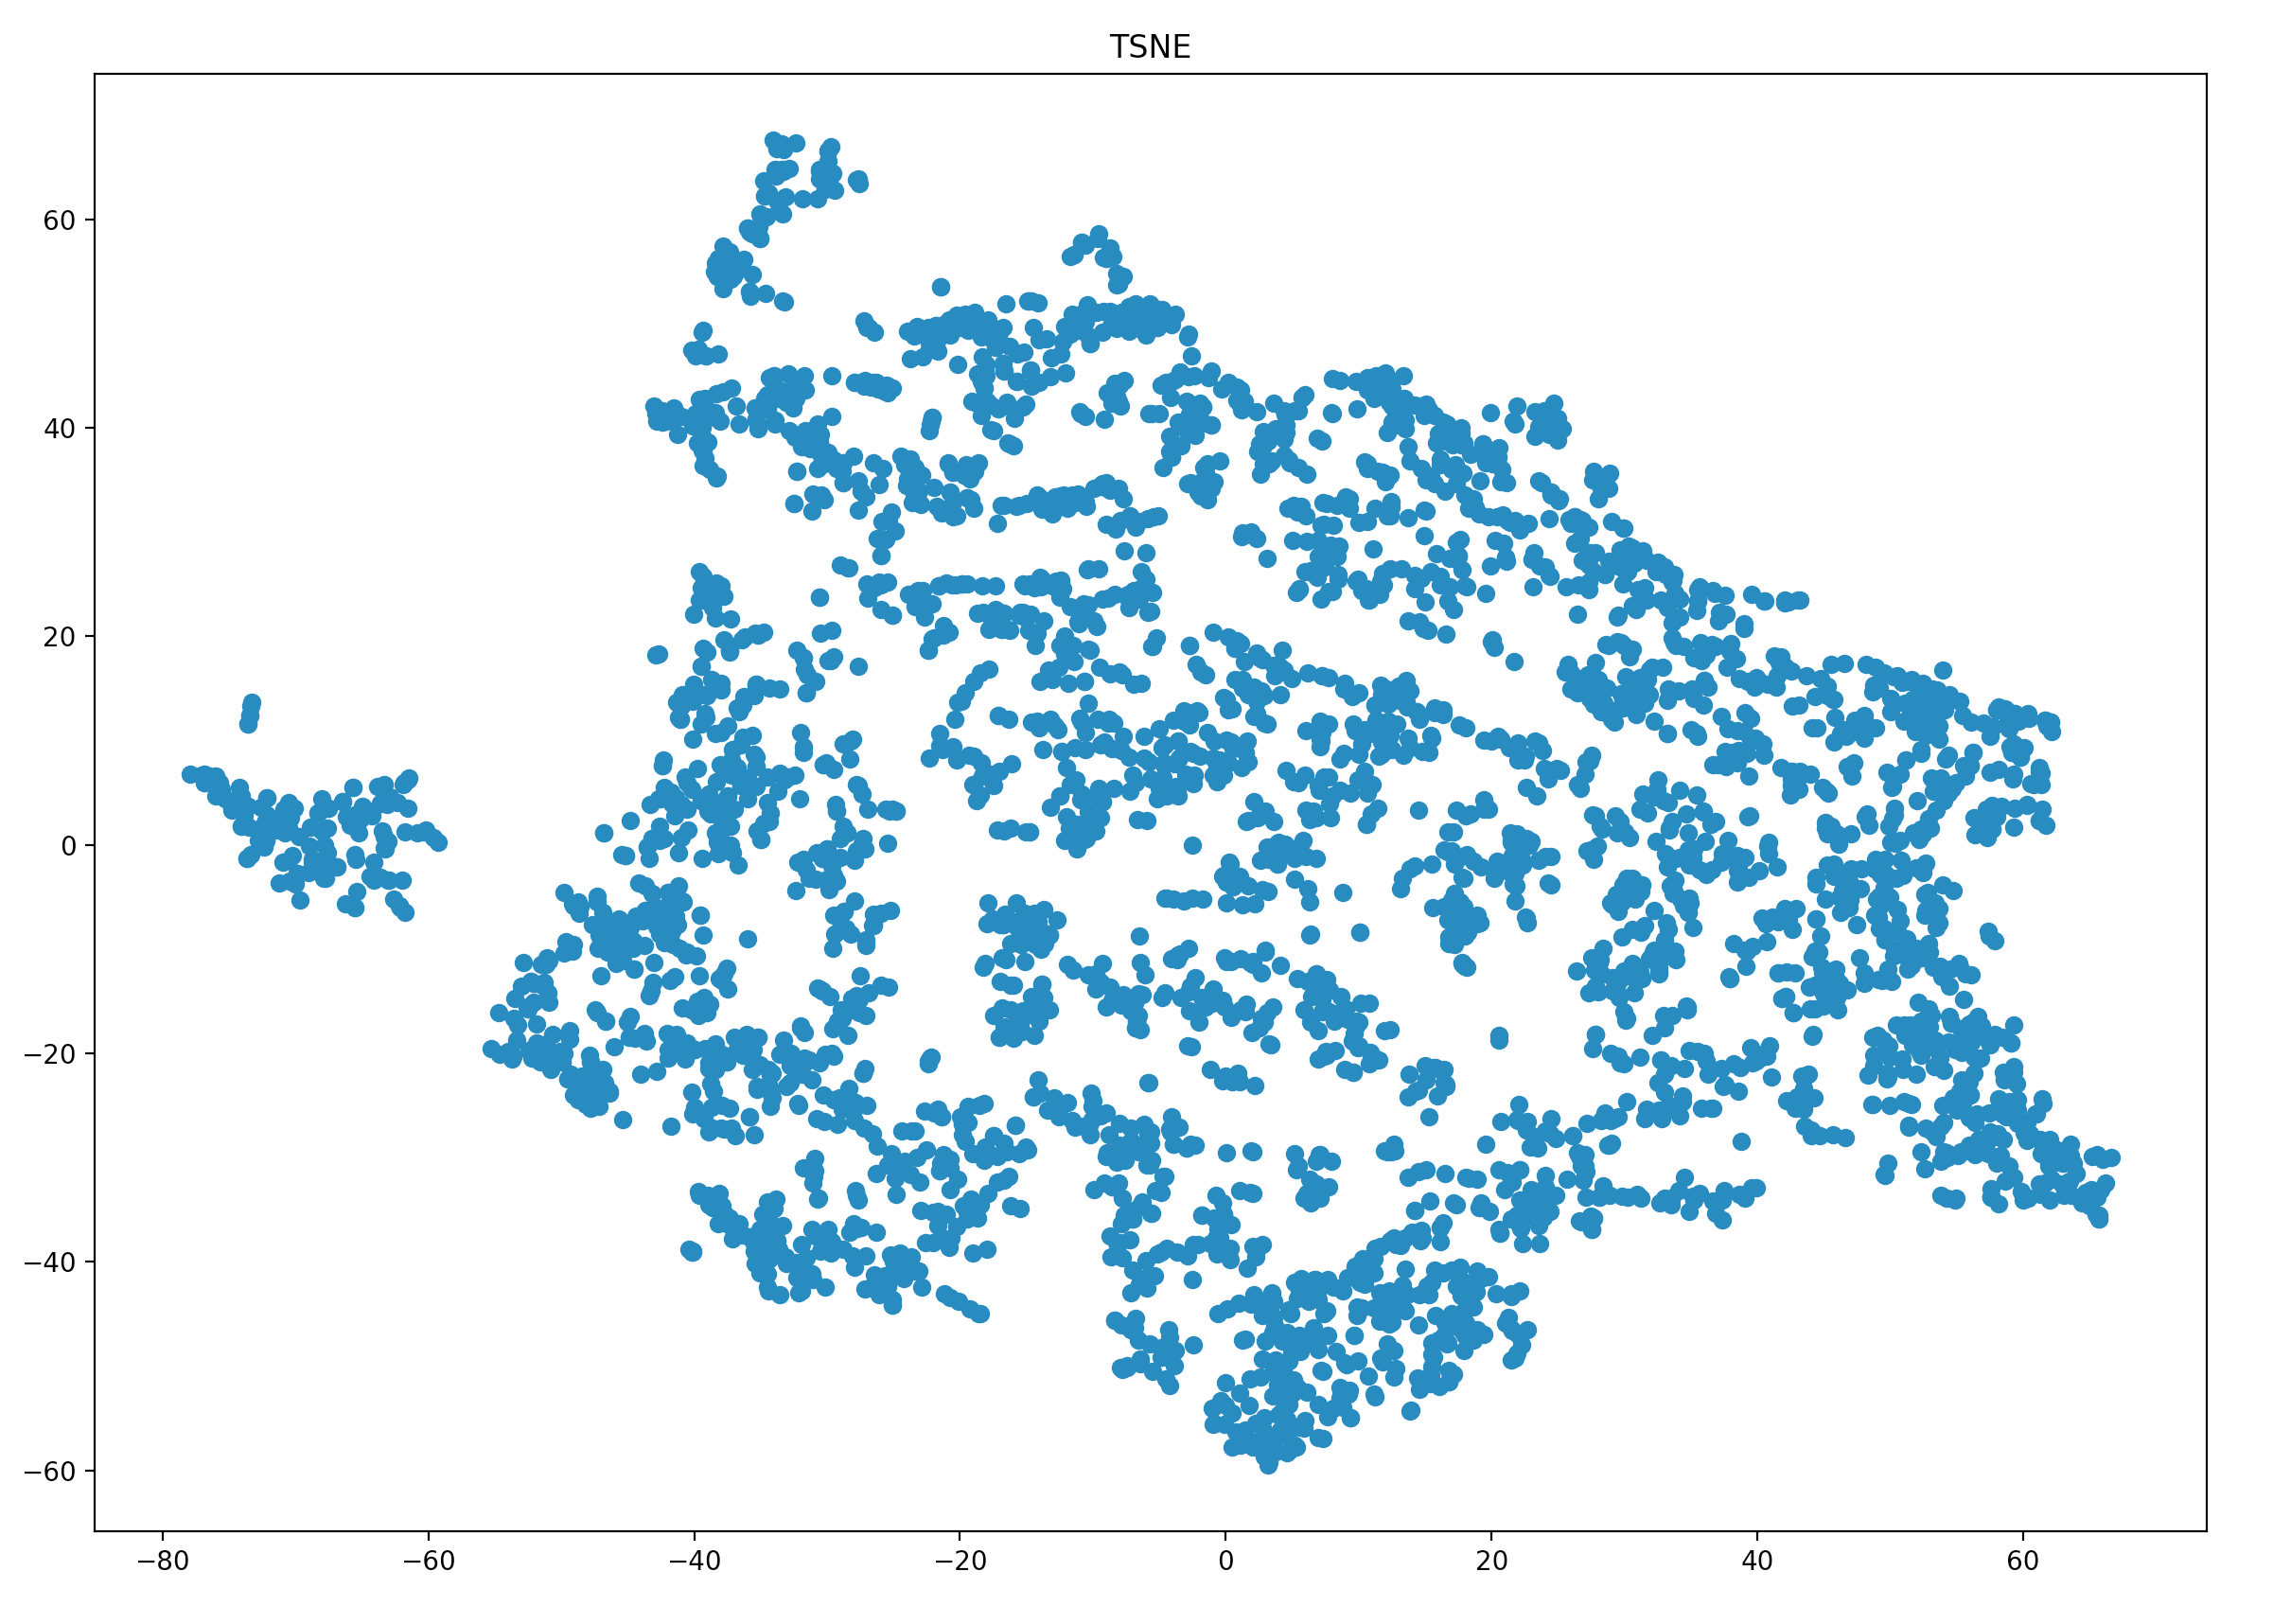
\includegraphics[width=0.9\textwidth]{./images/tsneParametersTest/learningRate/lr10-3hTSNE.png}
  \end{subfigure}%
  \begin{subfigure}{.5\textwidth}
    \centering
    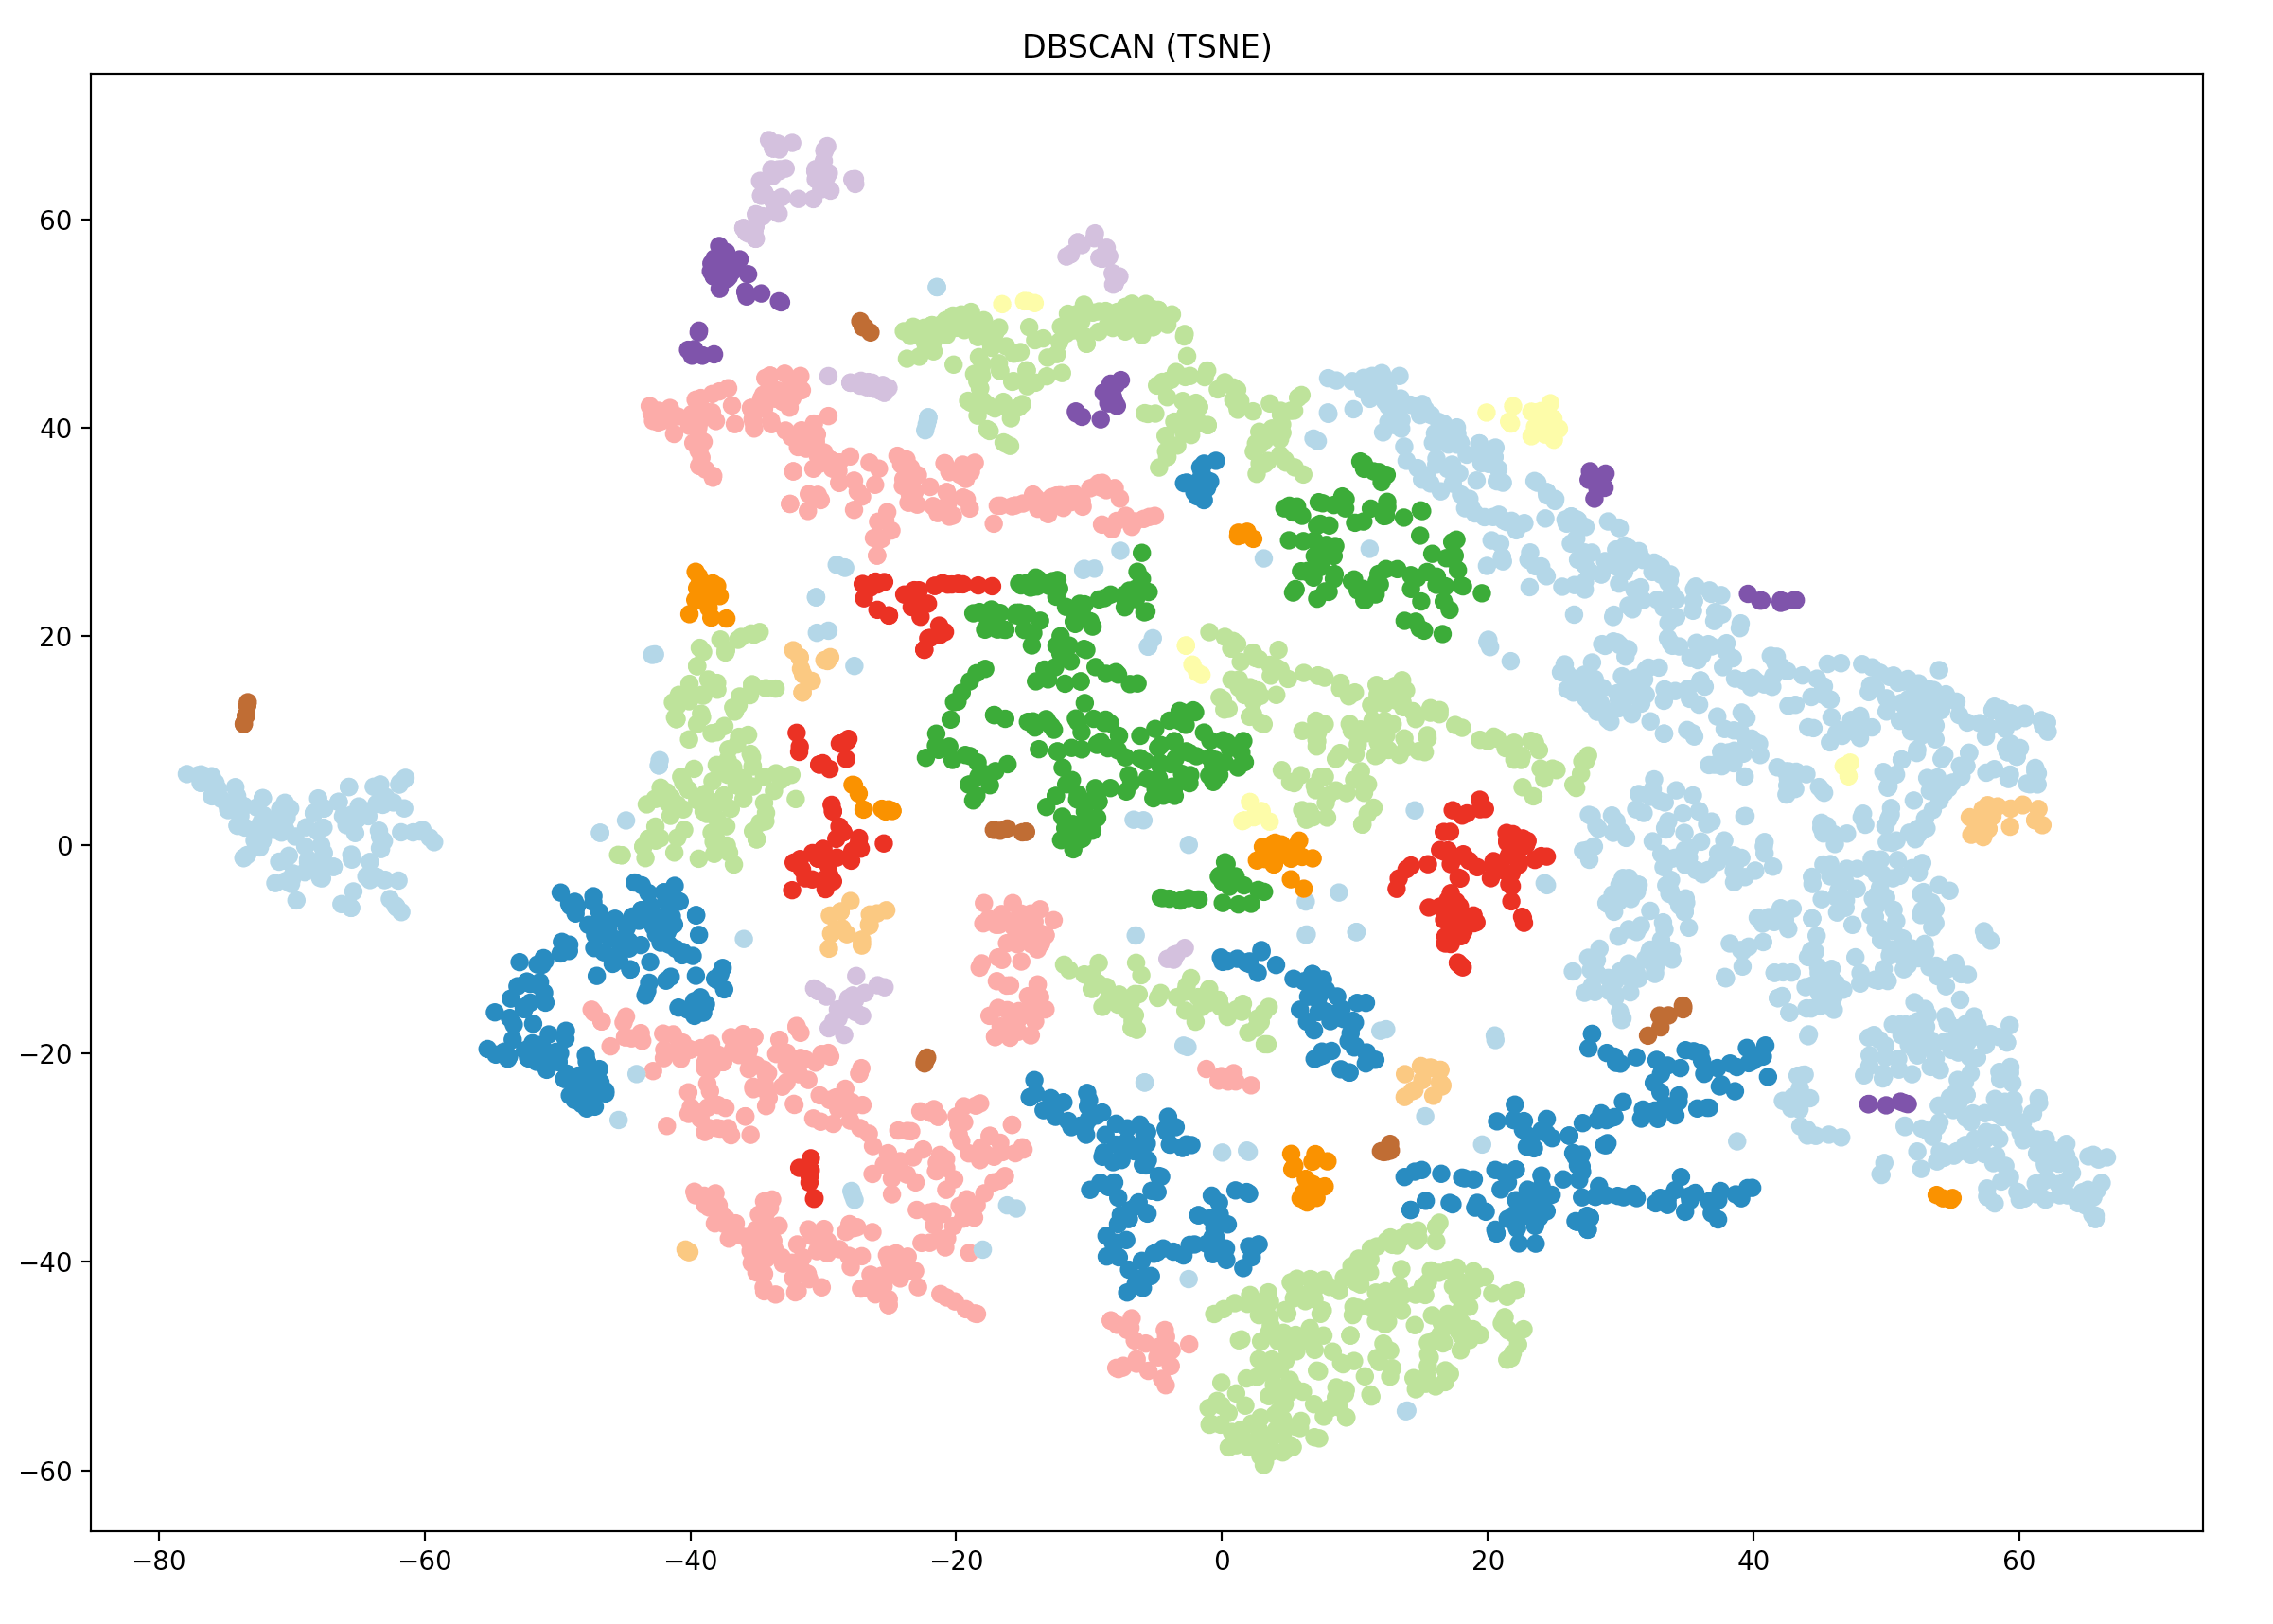
\includegraphics[width=0.9\textwidth]{./images/tsneParametersTest/learningRate/lr10-3hDBSCAN.png}
	\end{subfigure}
	\caption{\textbf{3h} data files, t-SNE calculated with the following parameters: perplexity=40, n\_iter=5000, \textbf{learning\_rate=10}}
  \label{figure:3hlr10TSNE}
\end{figure}

%------------------ LEARNING RATE 200: ------------------
\subsubsection{Learning Rate = 200}
% -- 1h, lr 200 --
\begin{figure}[H]
  \centering
  \begin{subfigure}{.5\textwidth}
    \centering
    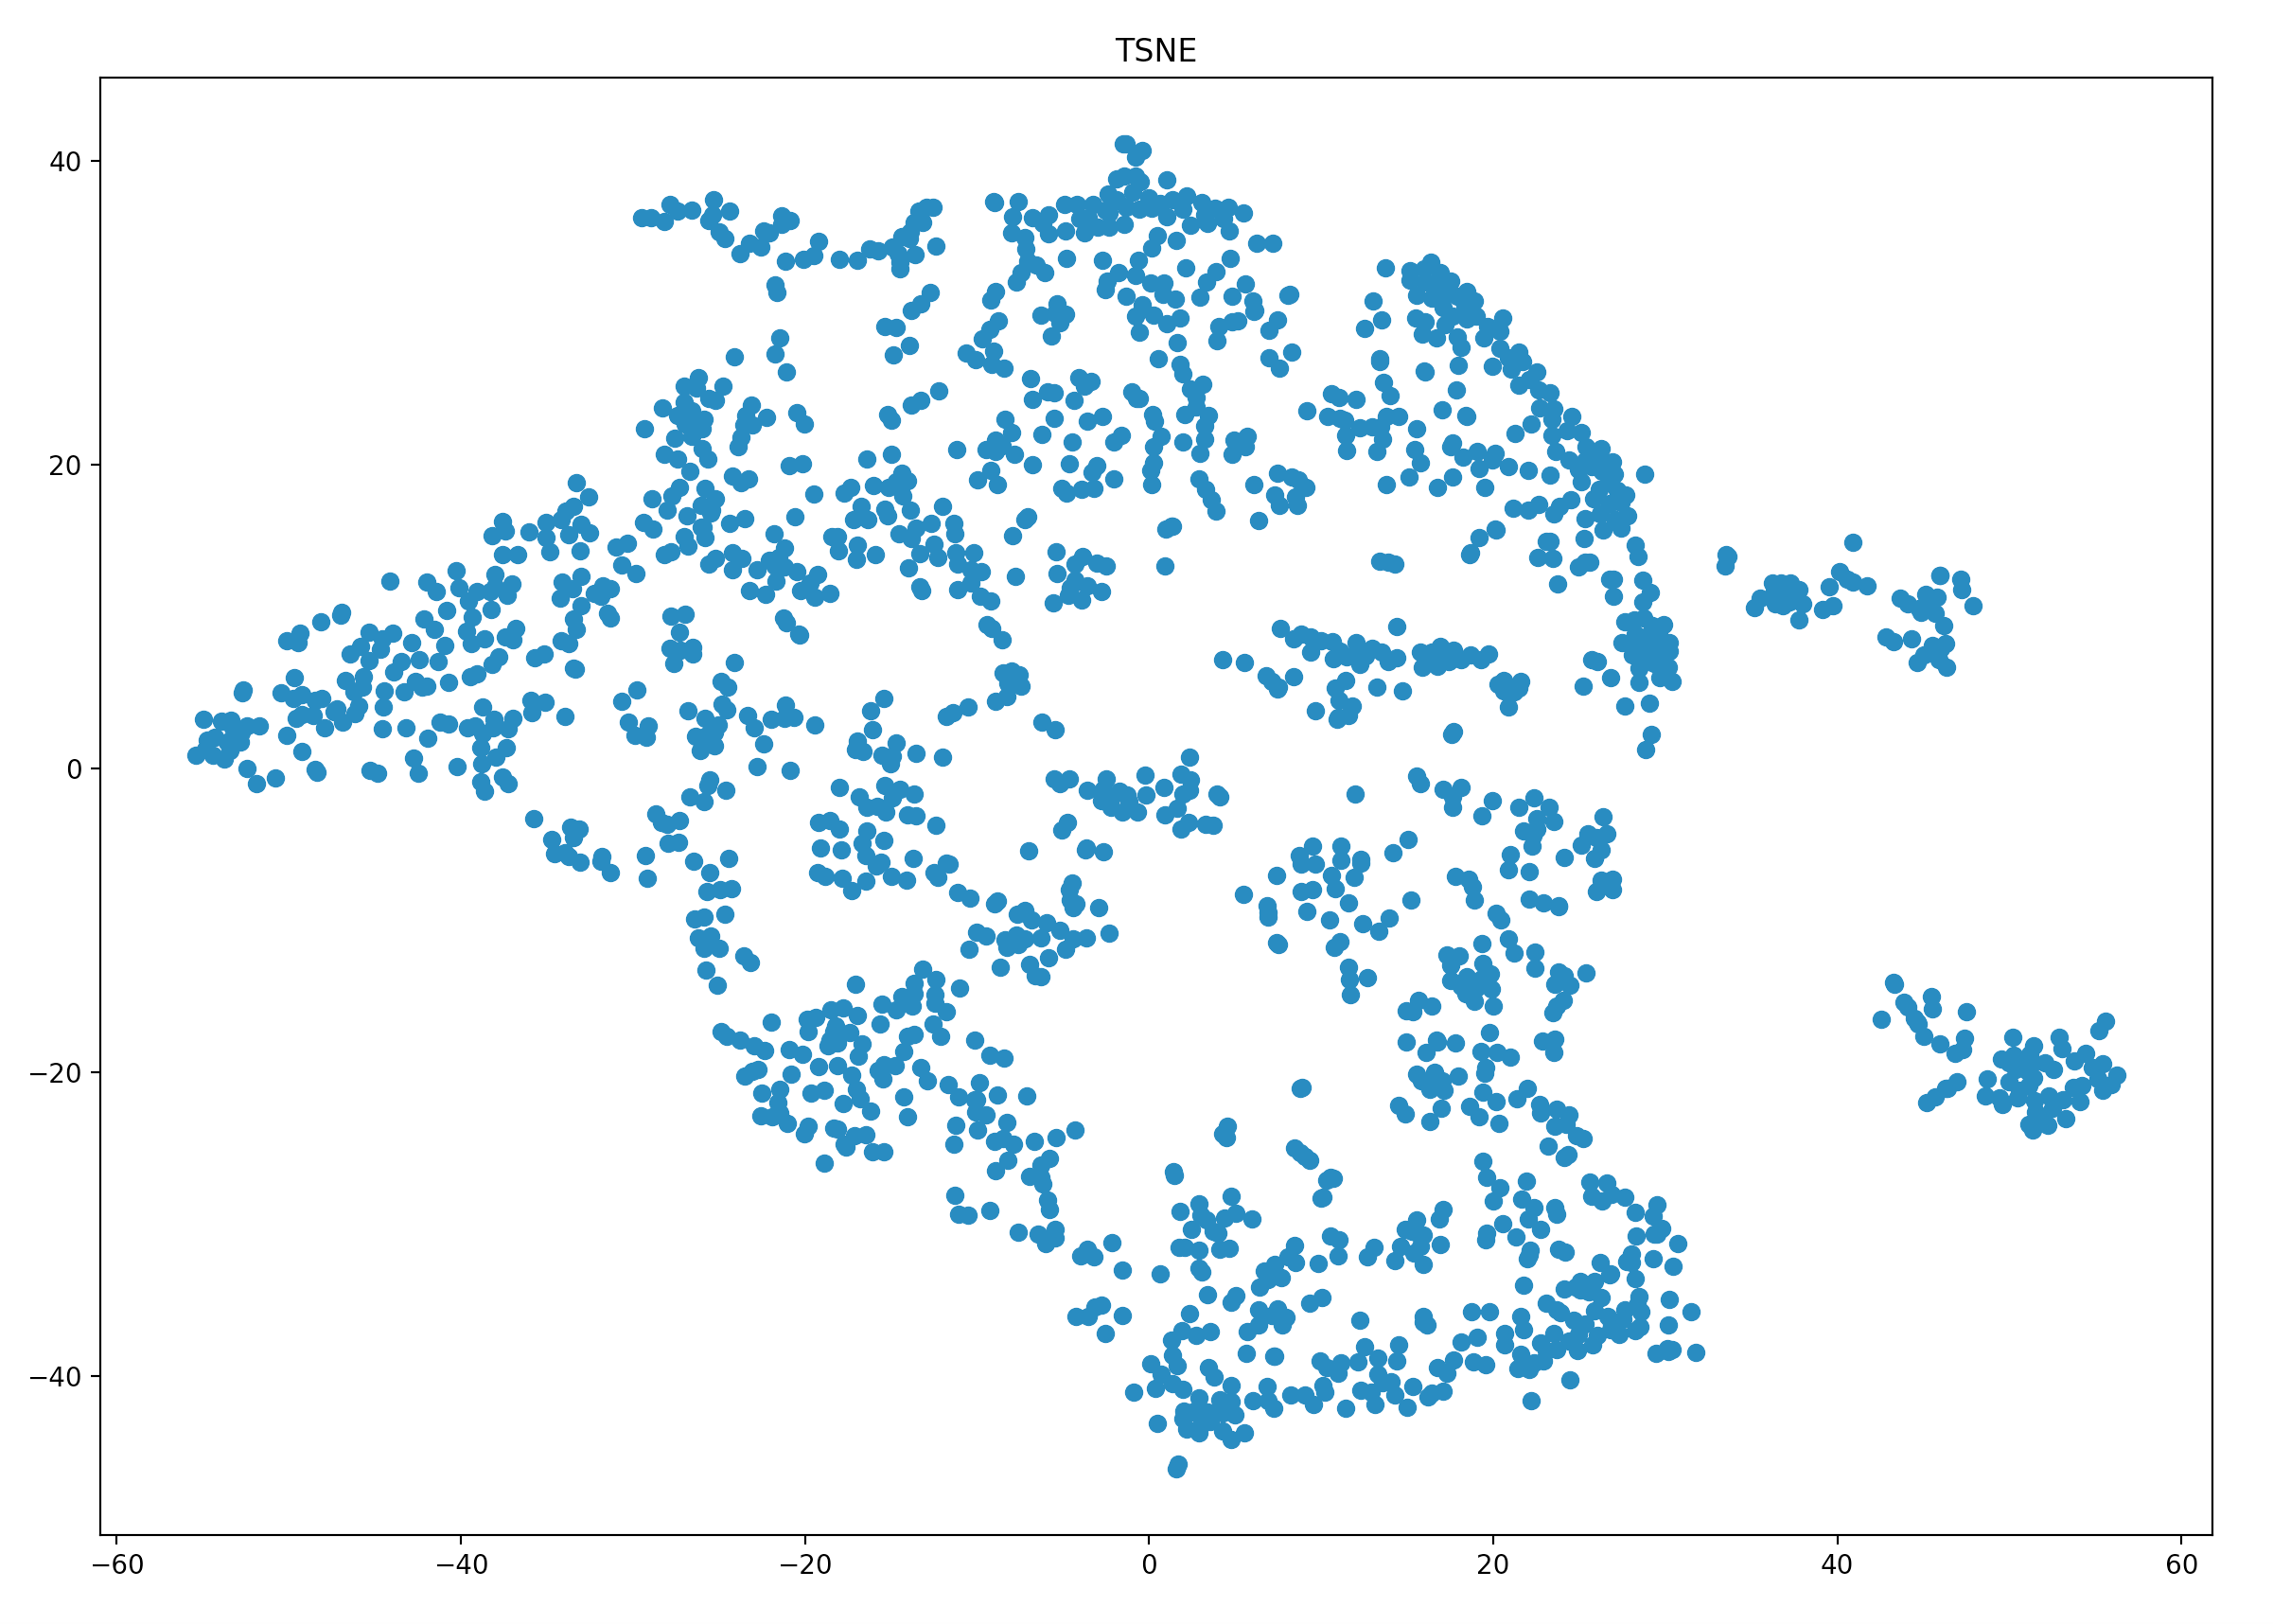
\includegraphics[width=0.9\textwidth]{./images/tsneParametersTest/learningRate/lr200-1hTSNE.png}
  \end{subfigure}%
  \begin{subfigure}{.5\textwidth}
    \centering
    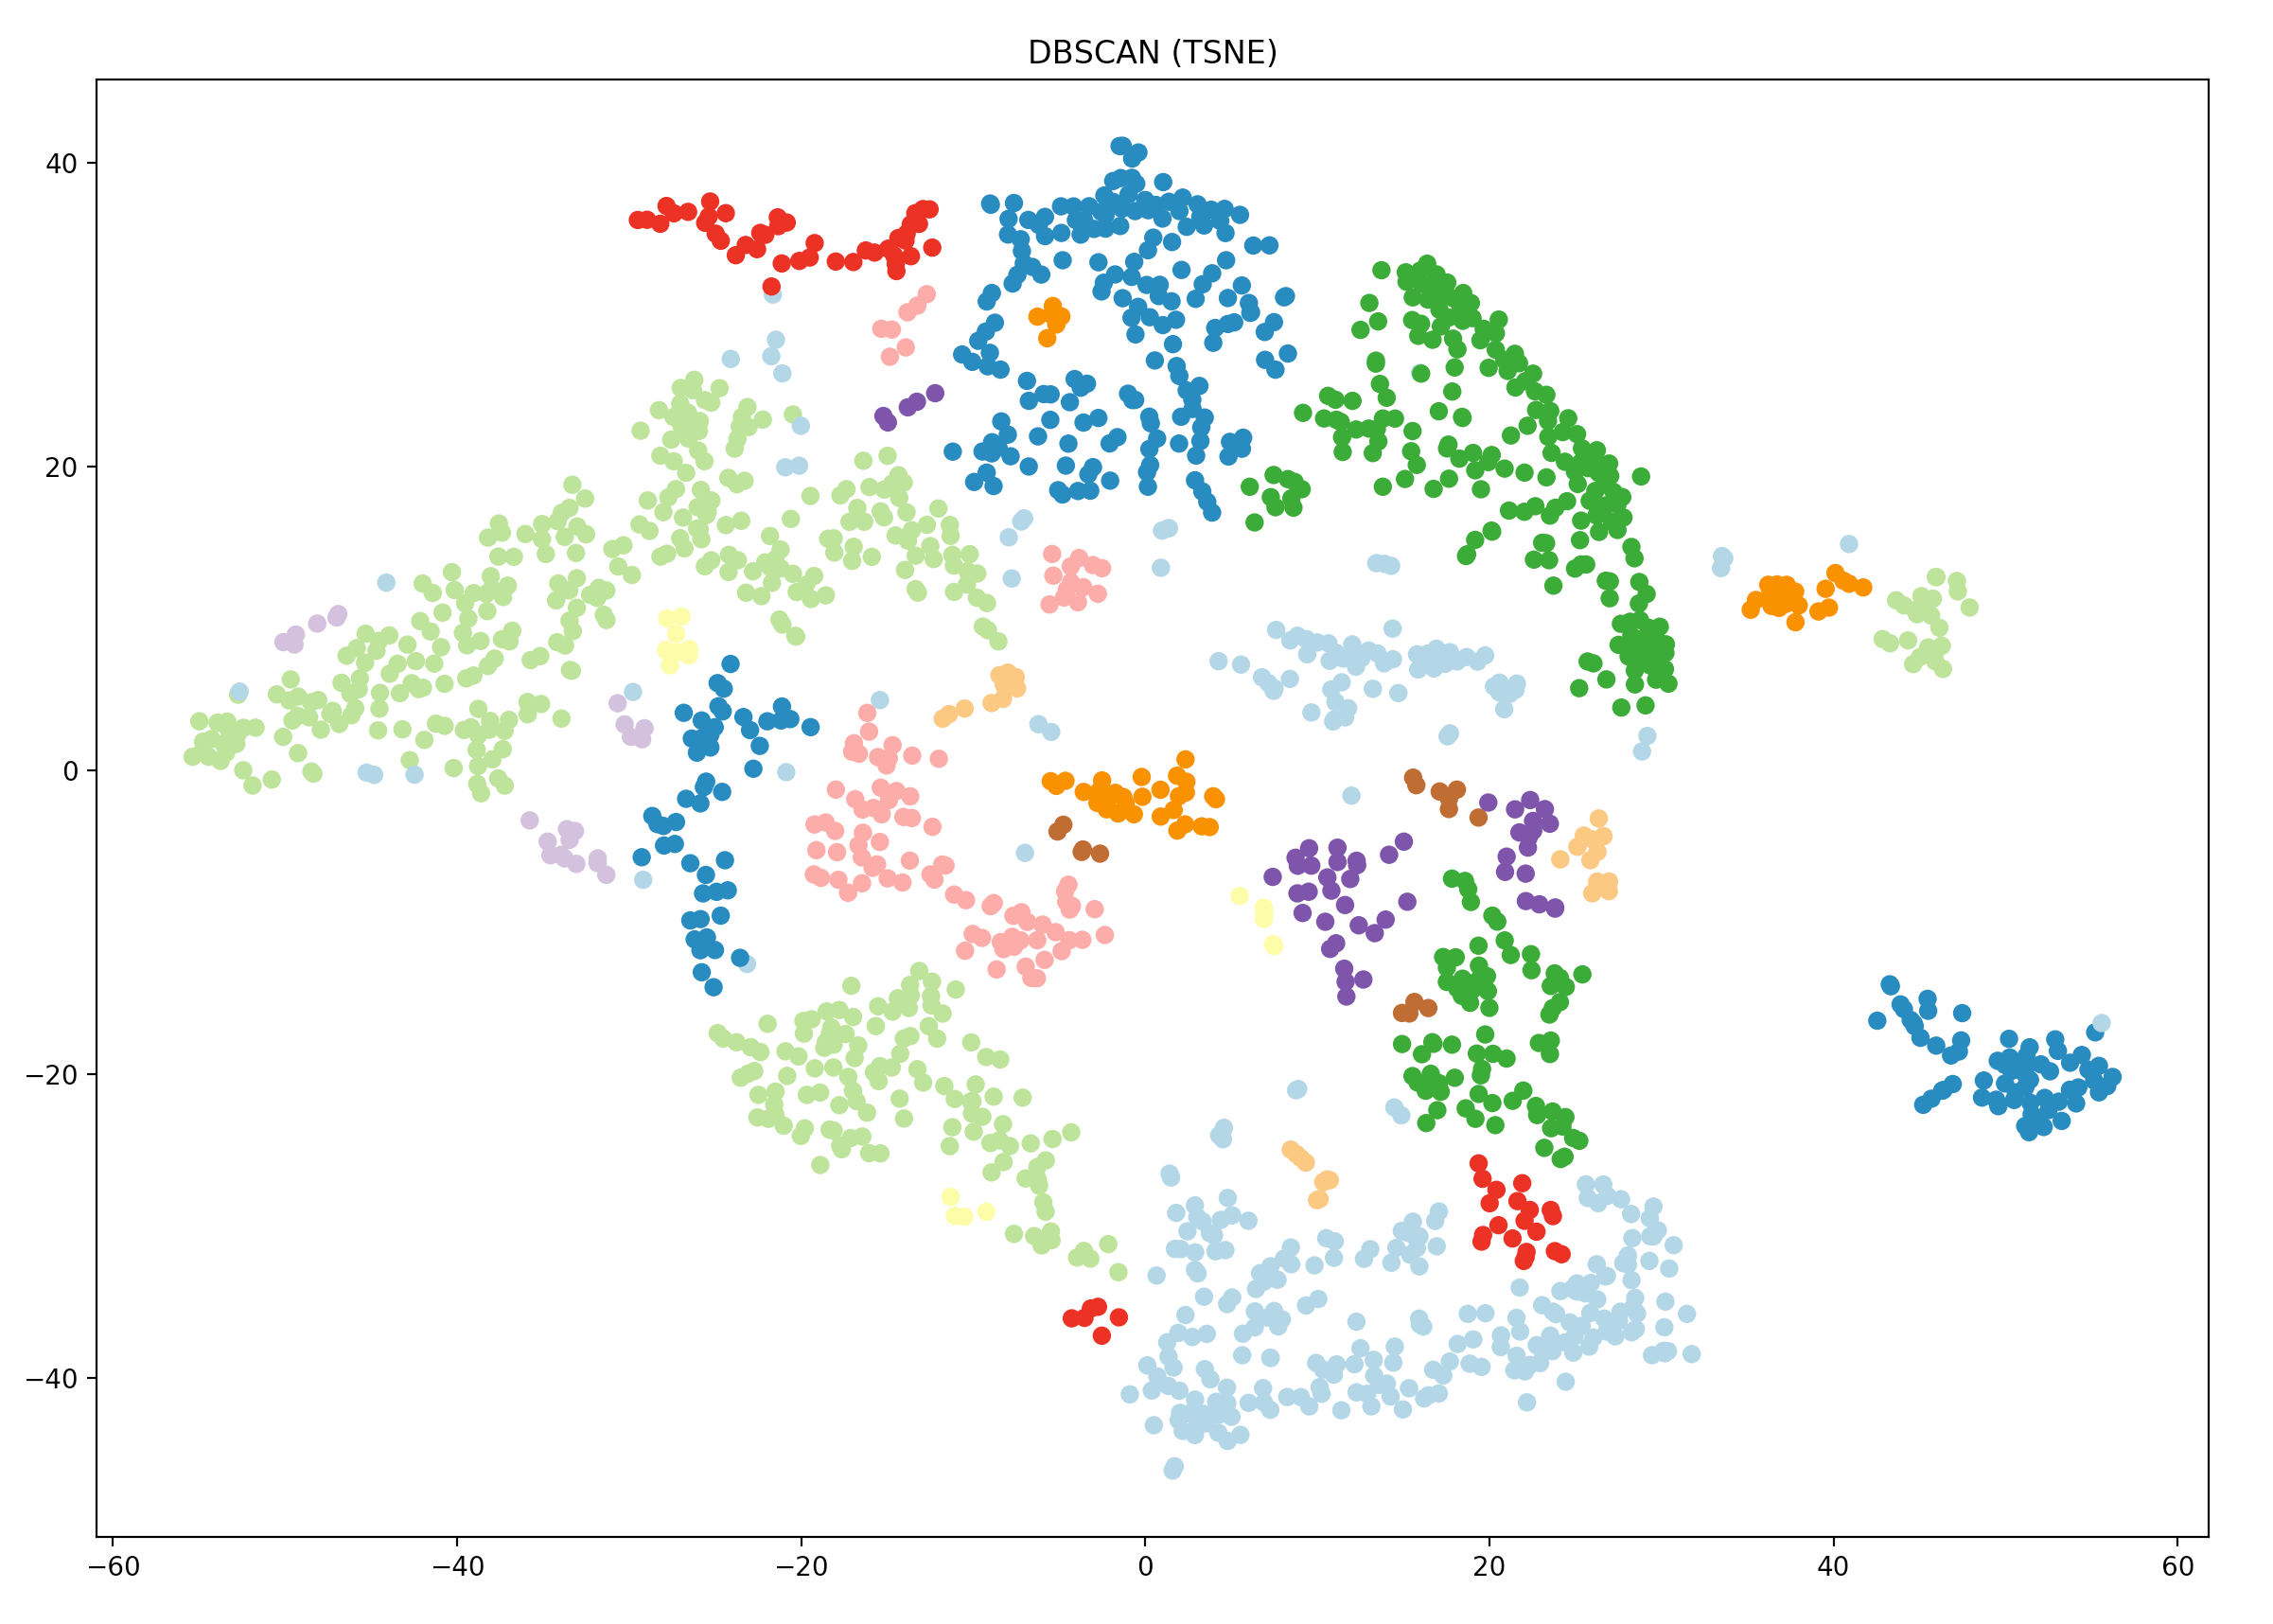
\includegraphics[width=0.9\textwidth]{./images/tsneParametersTest/learningRate/lr200-1hDBSCAN.png}
  \end{subfigure}
	\caption{\textbf{1h} data files, t-SNE calculated with the following parameters: perplexity=40, n\_iter=5000, \textbf{learning\_rate=200}}
	\label{figure:1hlr200TSNE}
\end{figure}

% -- 3h, lr 200 --
\begin{figure}[H]
	\centering
	
  \centering
	\begin{subfigure}{.5\textwidth}
    \centering
    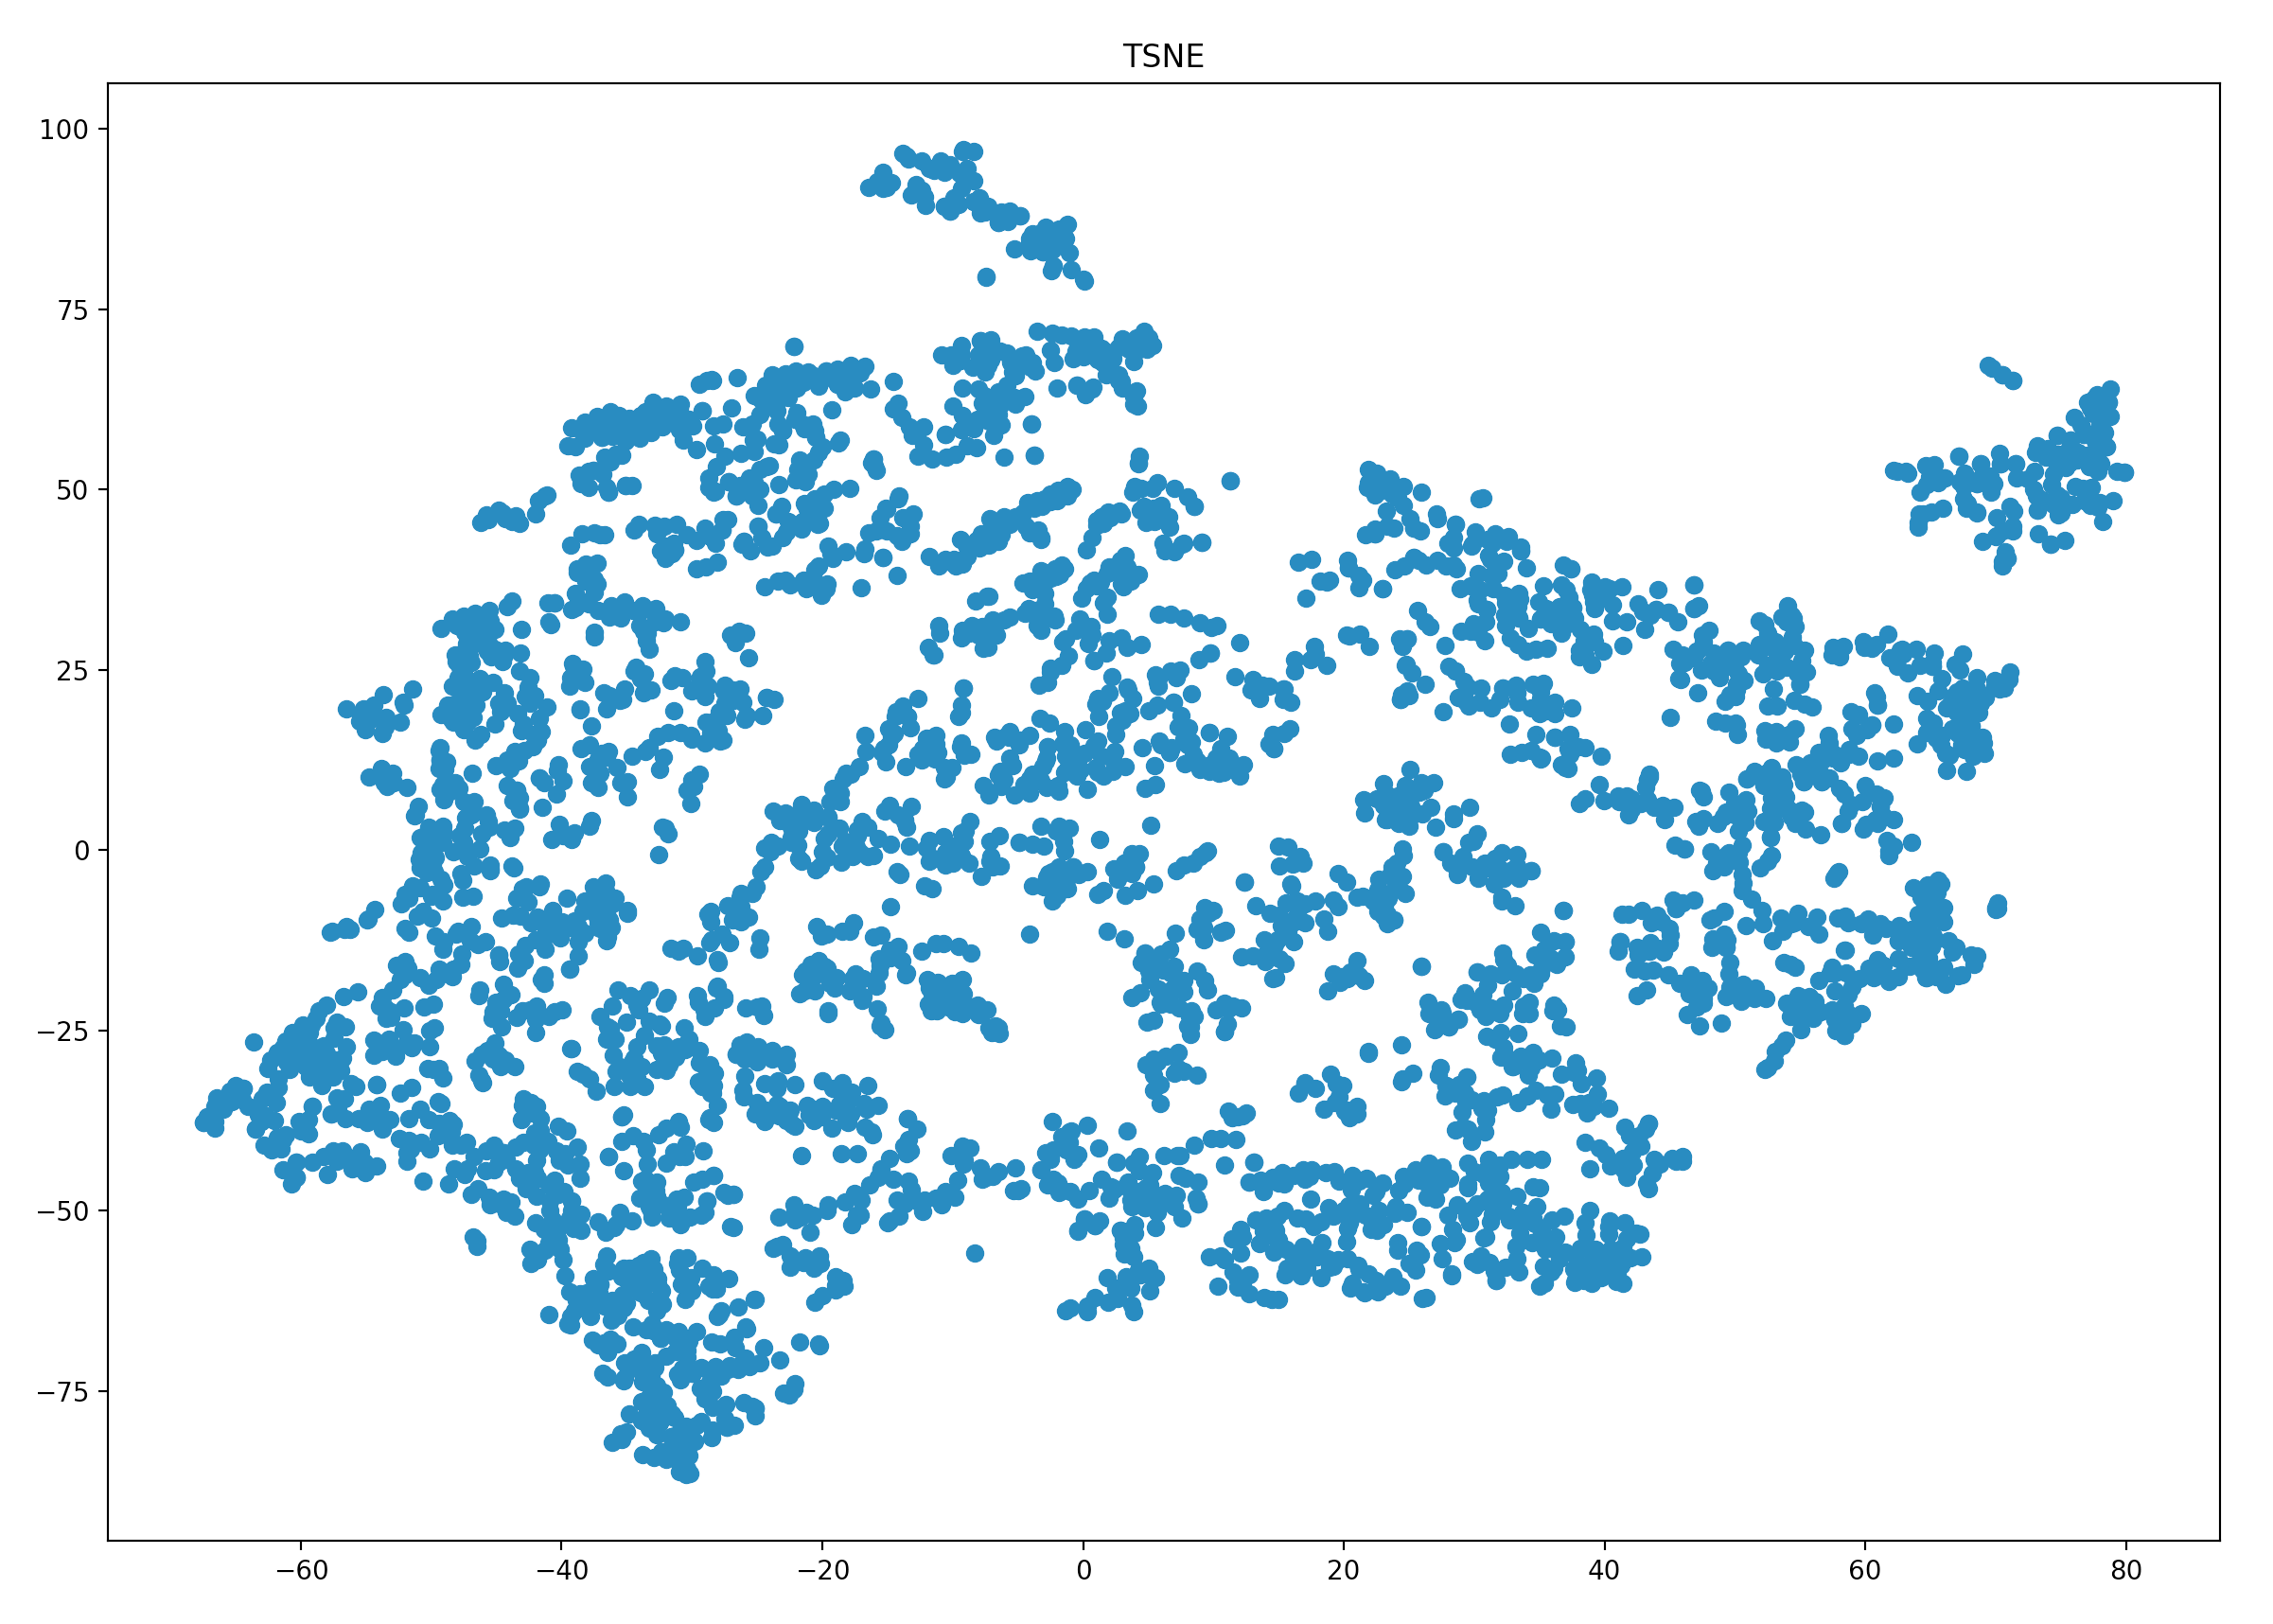
\includegraphics[width=0.9\textwidth]{./images/tsneParametersTest/learningRate/lr200-3hTSNE.png}
  \end{subfigure}%
  \begin{subfigure}{.5\textwidth}
    \centering
    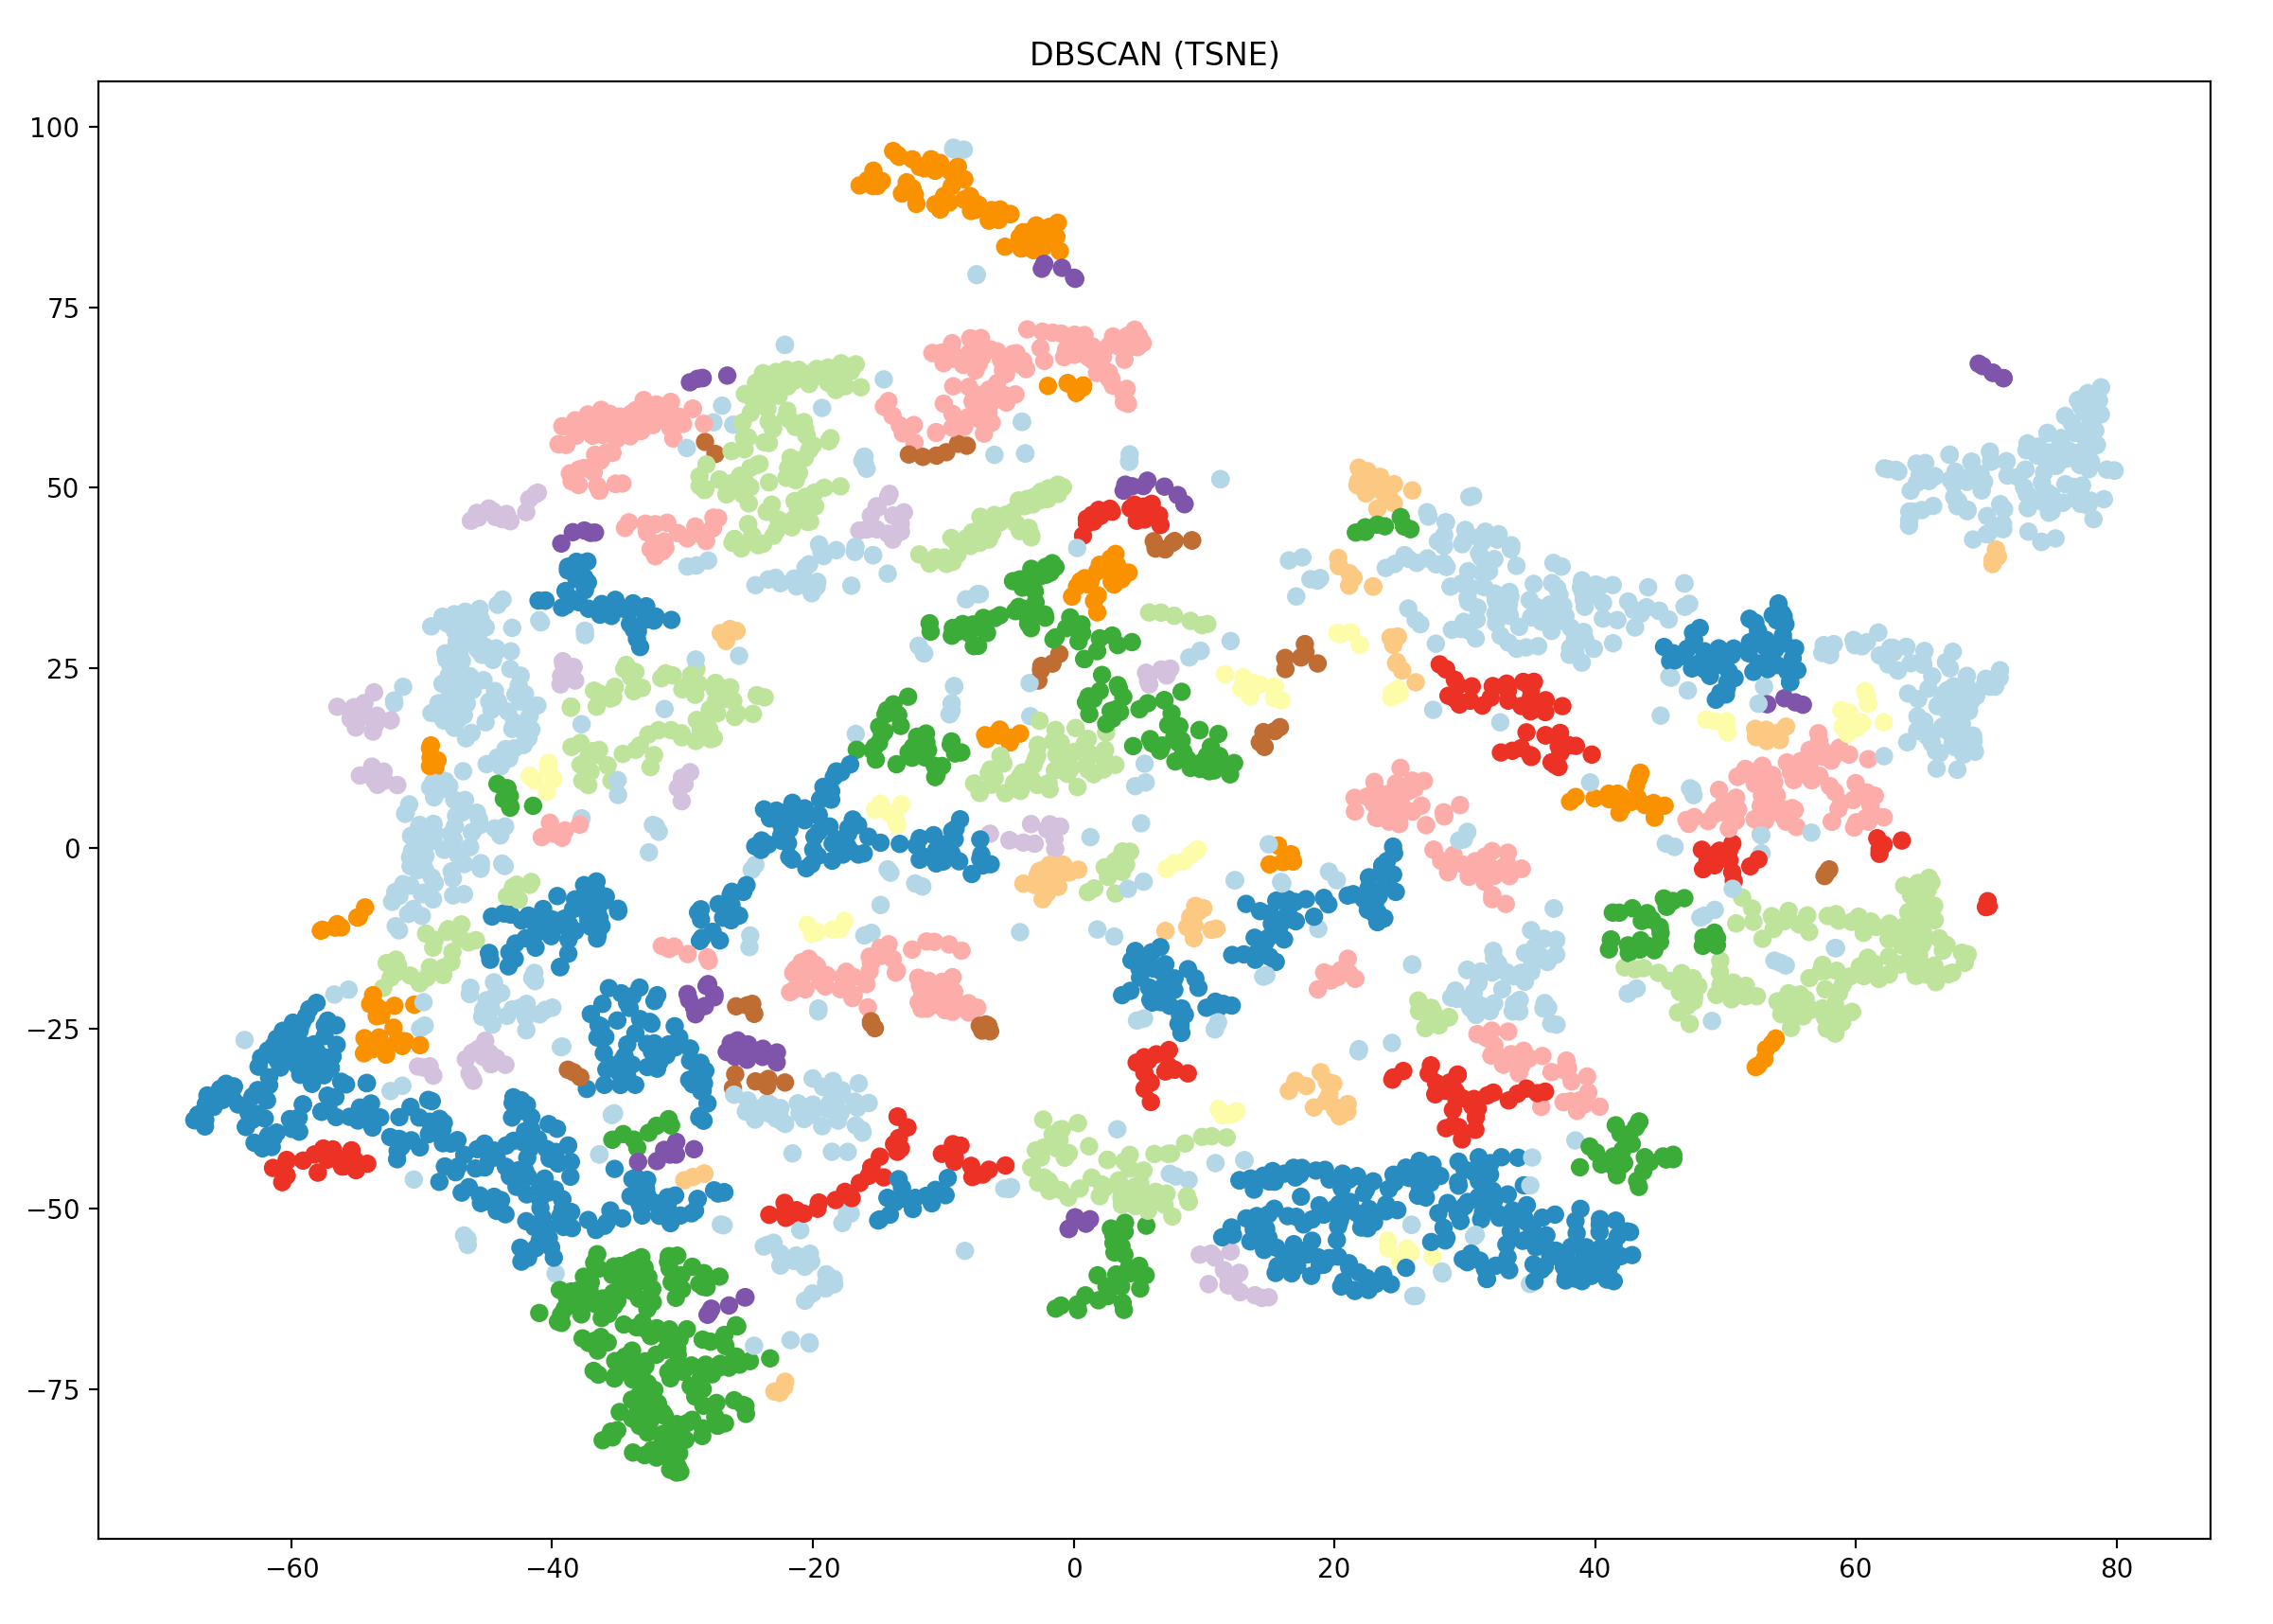
\includegraphics[width=0.9\textwidth]{./images/tsneParametersTest/learningRate/lr200-3hDBSCAN.png}
	\end{subfigure}
	\caption{\textbf{3h} data files, t-SNE calculated with the following parameters: perplexity=40, n\_iter=5000, \textbf{learning\_rate=200}}
  \label{figure:3hlr200TSNE}
\end{figure}


%------------------ LEARNING RATE 400: ------------------
\subsubsection{Learning Rate = 400}
% -- 1h, lr 400 --
\begin{figure}[H]
  \centering
  \begin{subfigure}{.5\textwidth}
    \centering
    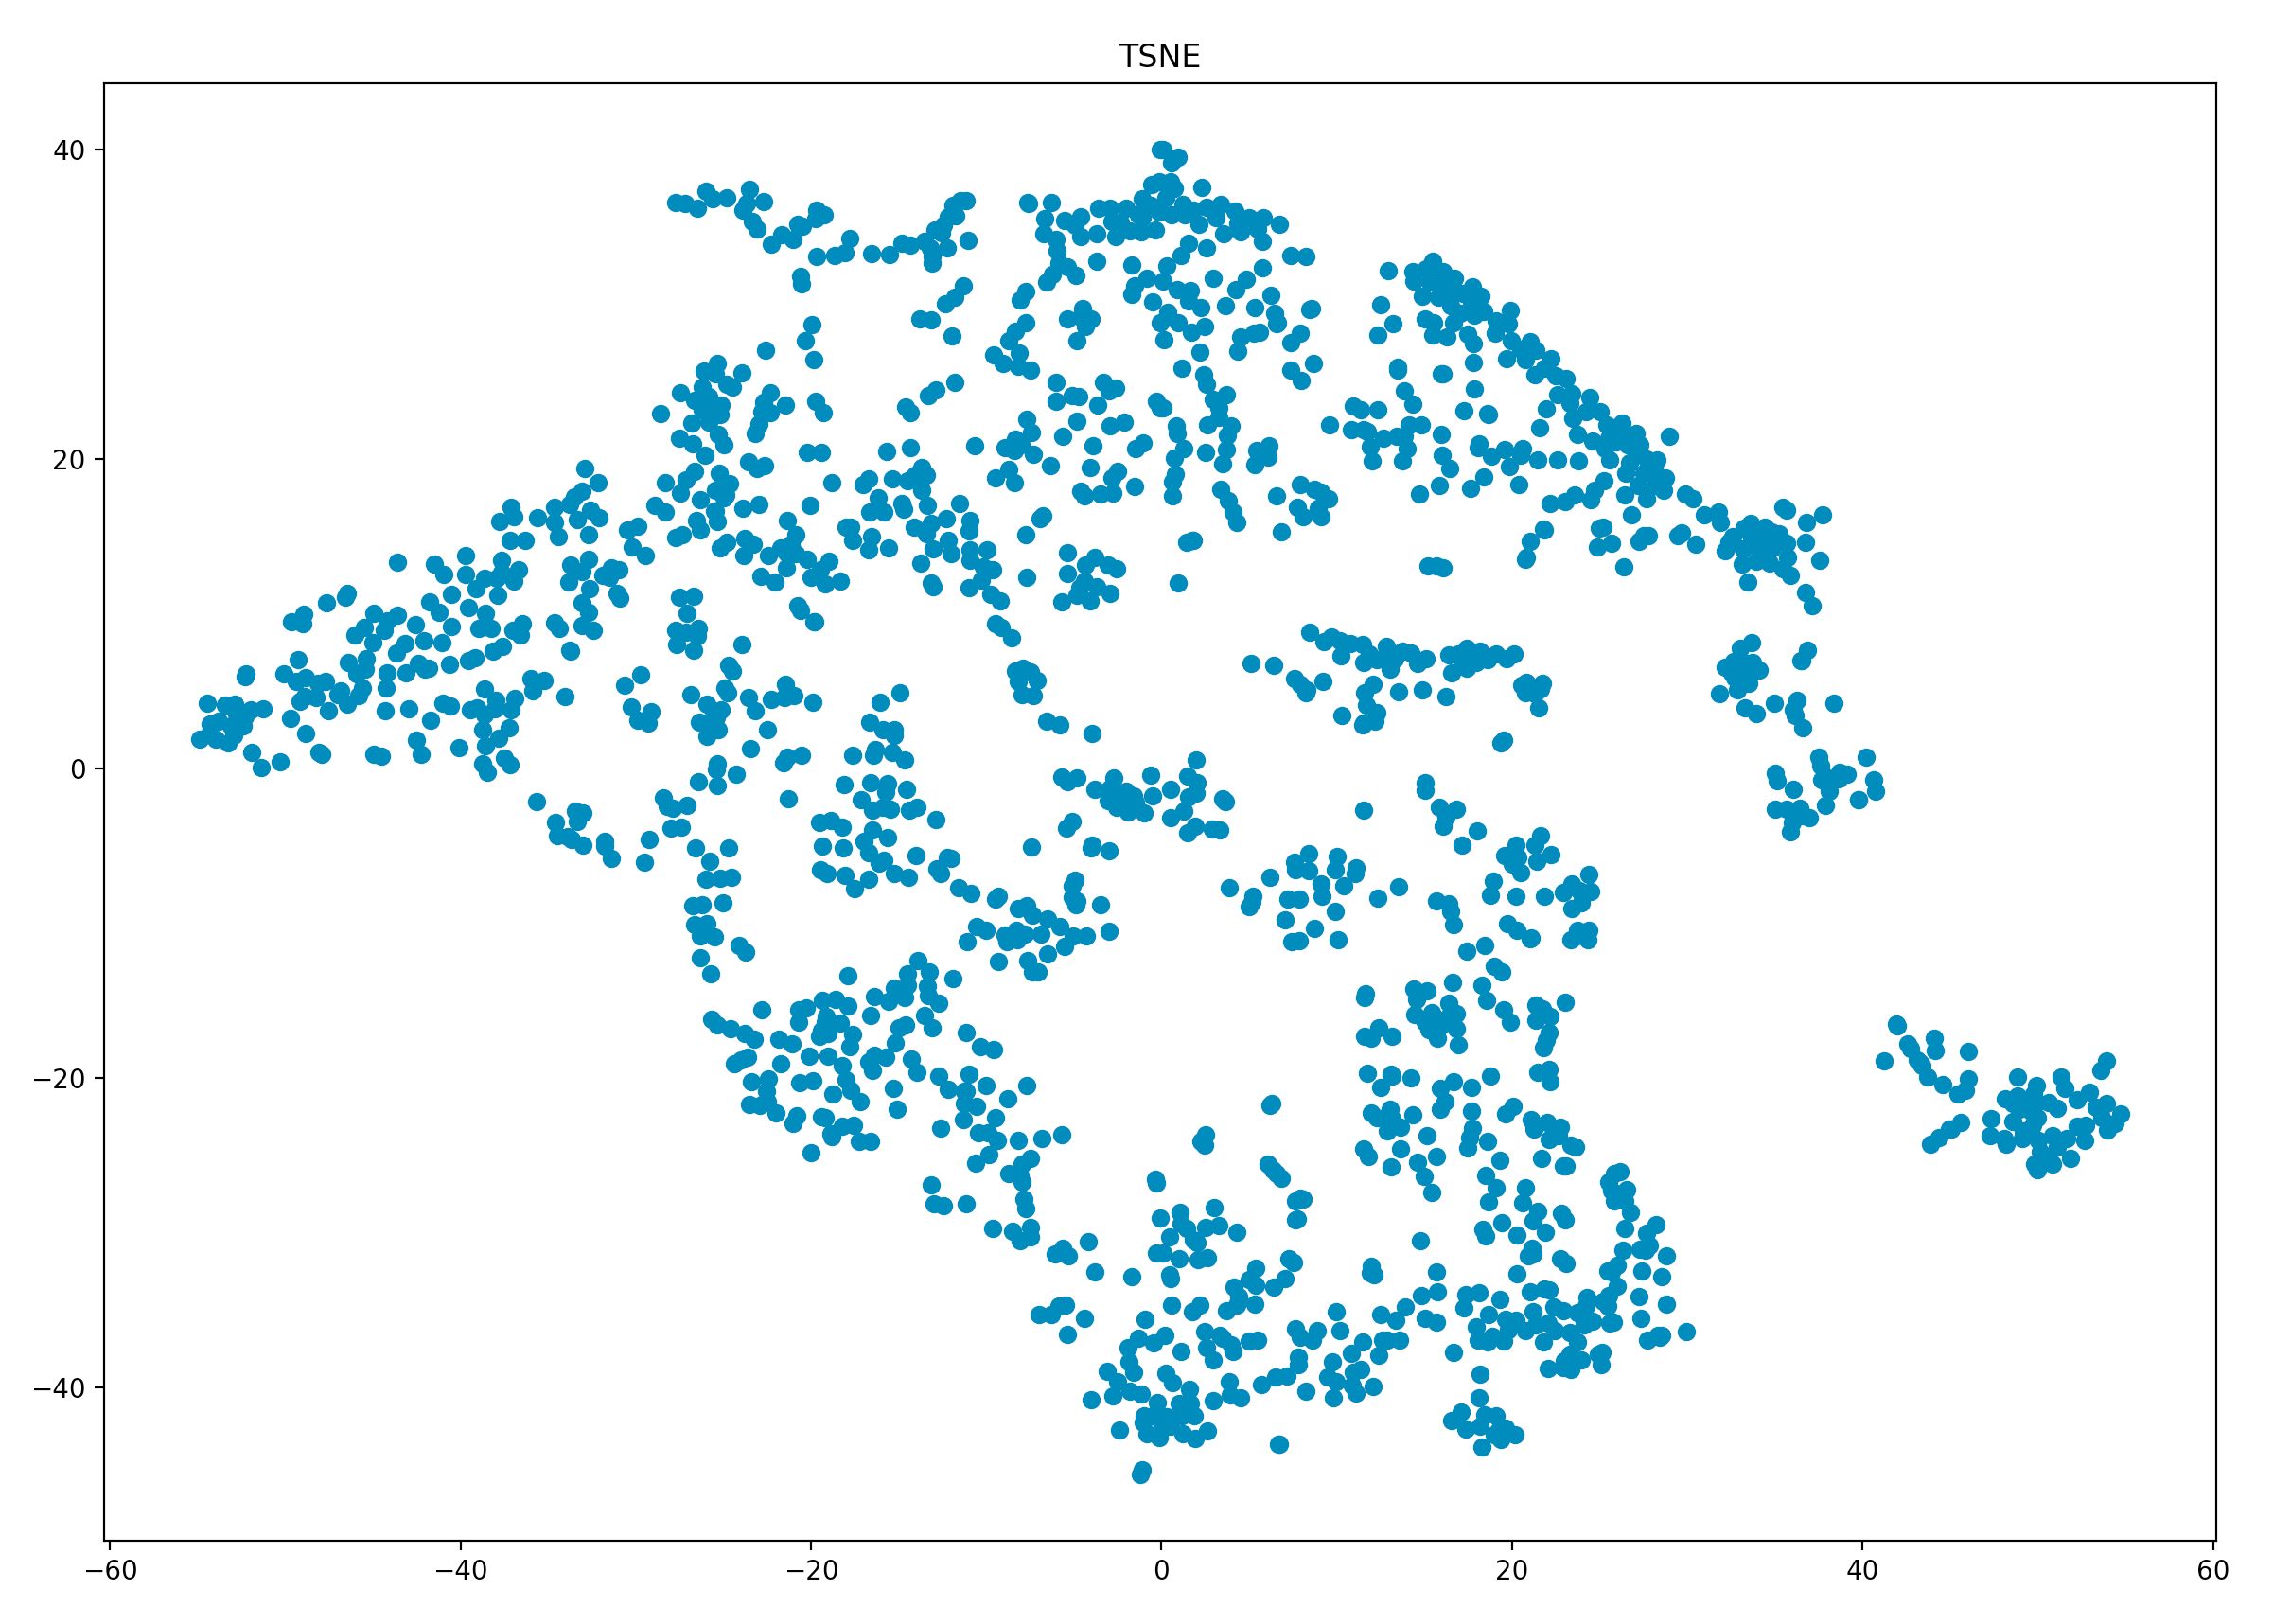
\includegraphics[width=0.9\textwidth]{./images/tsneParametersTest/learningRate/lr400-1hTSNE.png}
  \end{subfigure}%
  \begin{subfigure}{.5\textwidth}
    \centering
    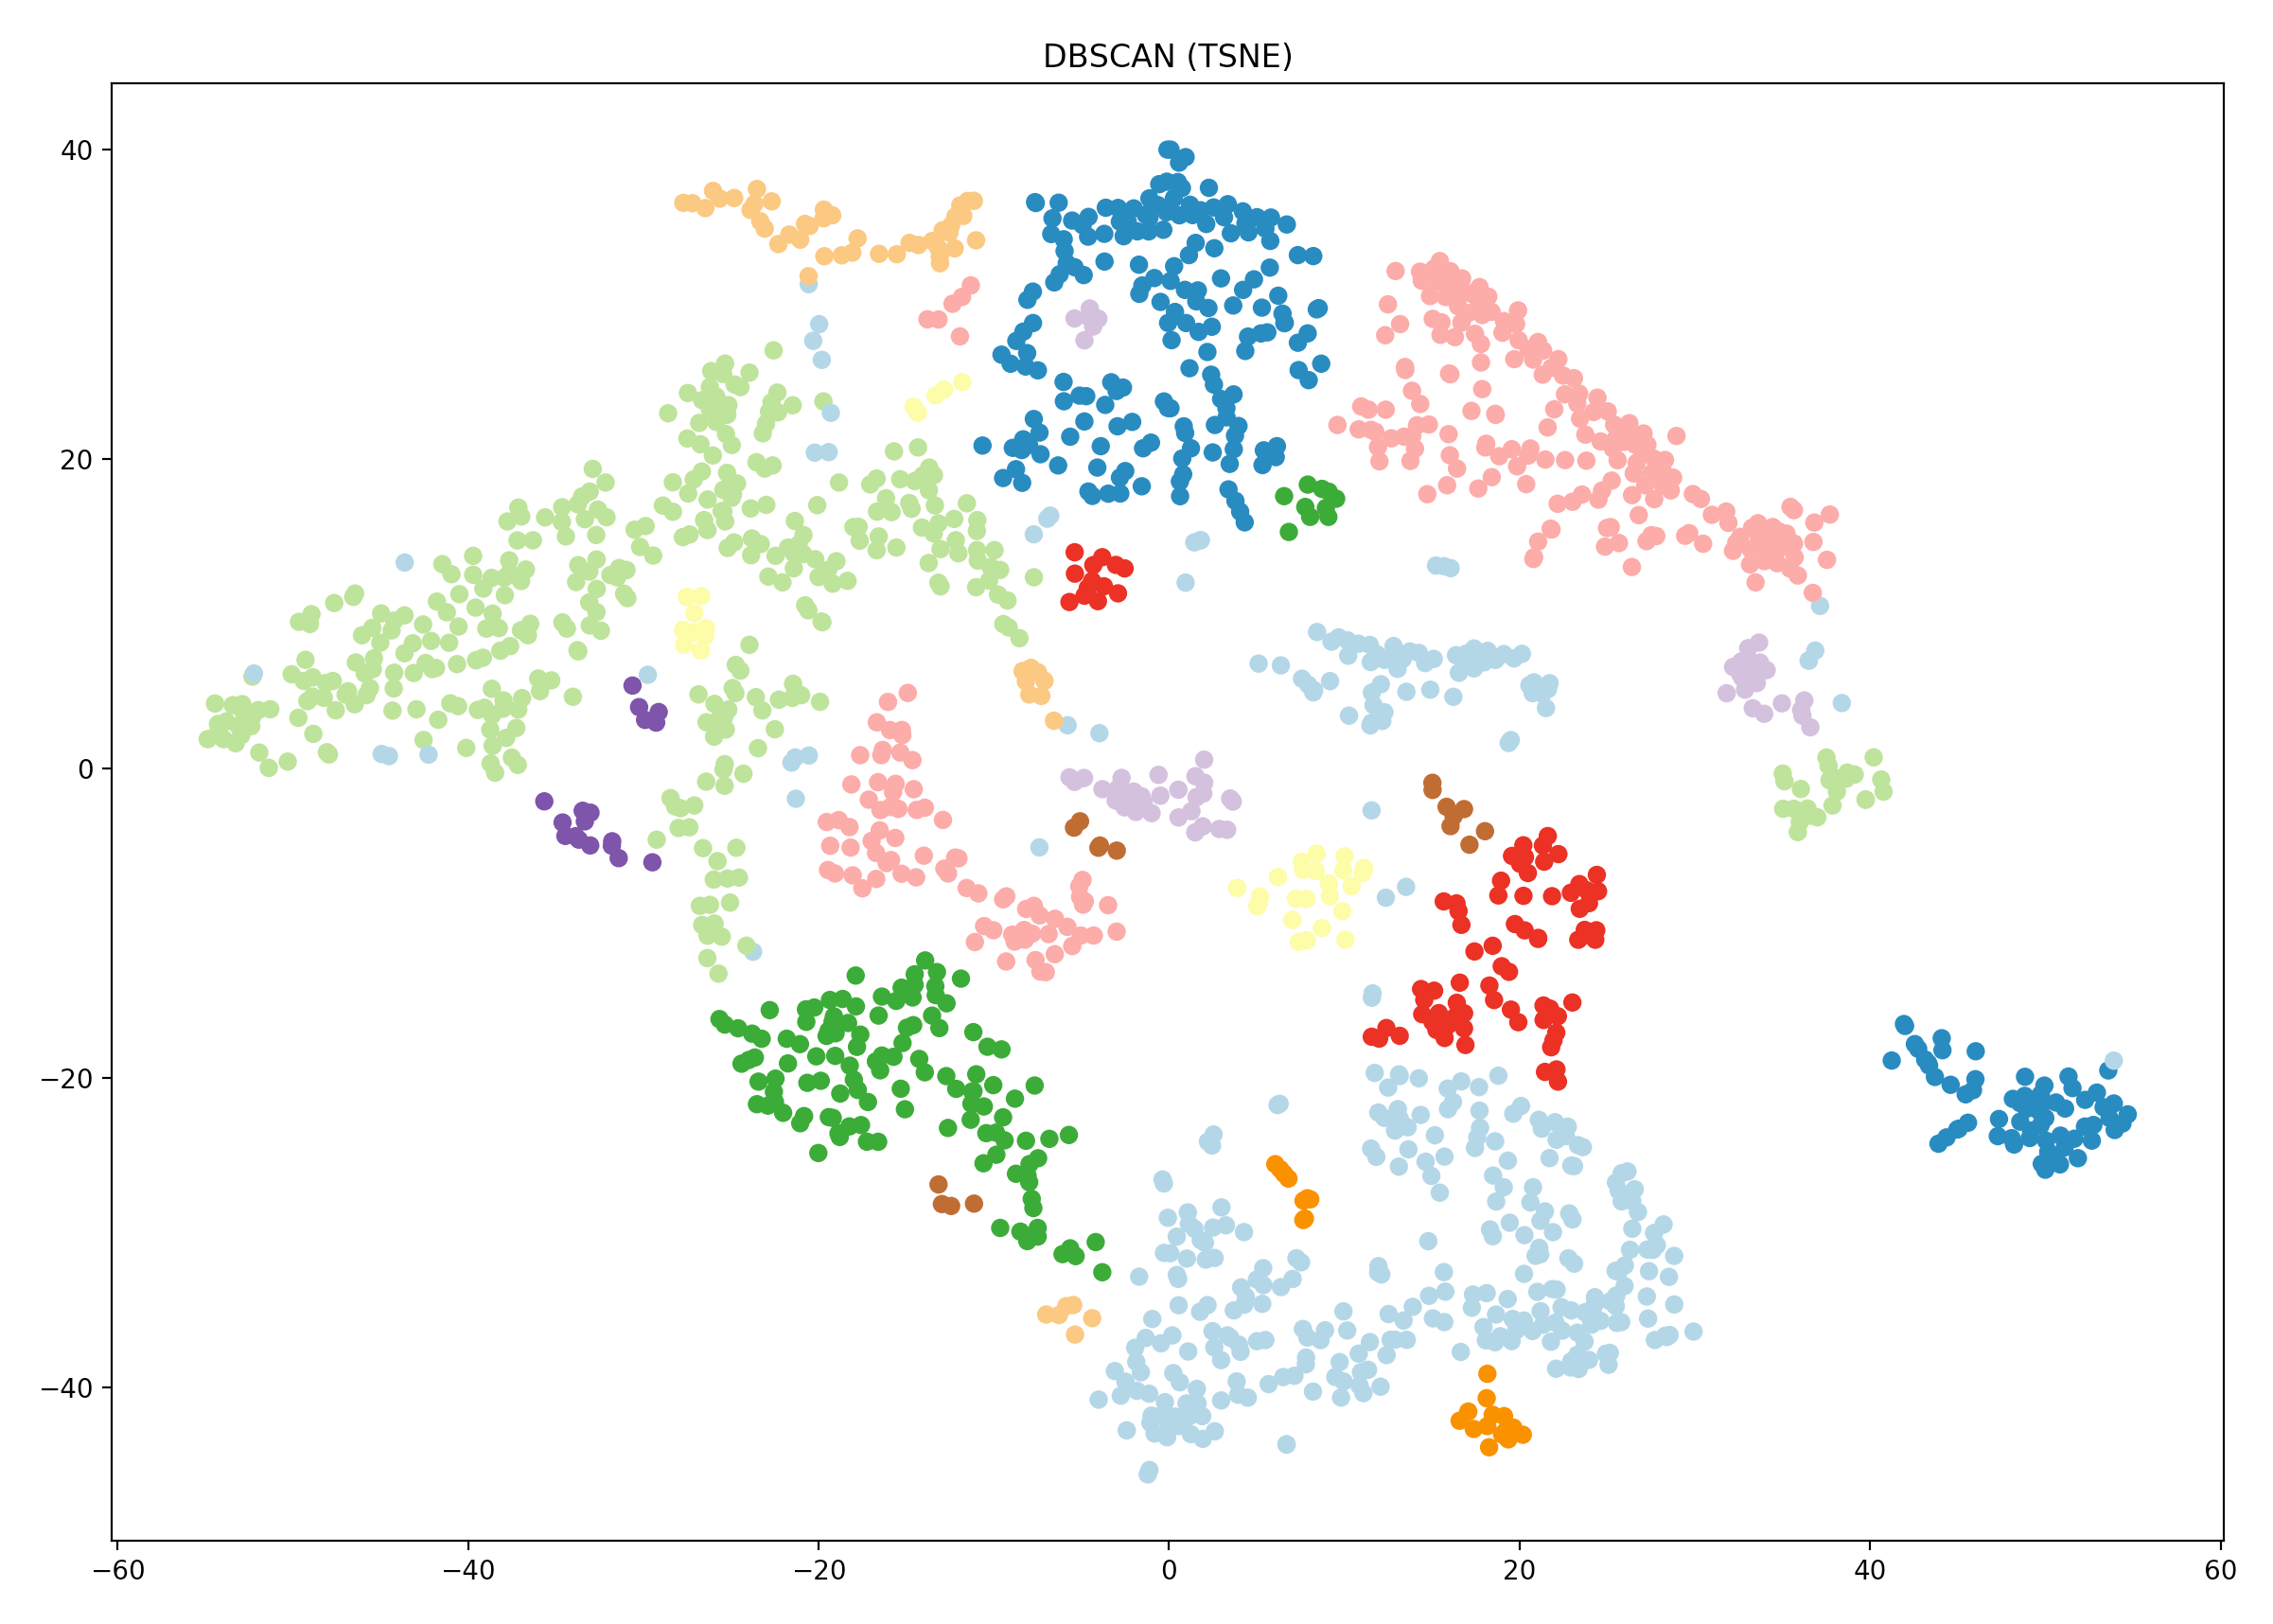
\includegraphics[width=0.9\textwidth]{./images/tsneParametersTest/learningRate/lr400-1hDBSCAN.png}
  \end{subfigure}
	\caption{\textbf{1h} data files, t-SNE calculated with the following parameters: perplexity=40, n\_iter=5000, \textbf{learning\_rate=400}}
	\label{figure:1hlr400TSNE}
\end{figure}

% -- 3h, lr 400 --
\begin{figure}[H]
	\centering
	
  \centering
	\begin{subfigure}{.5\textwidth}
    \centering
    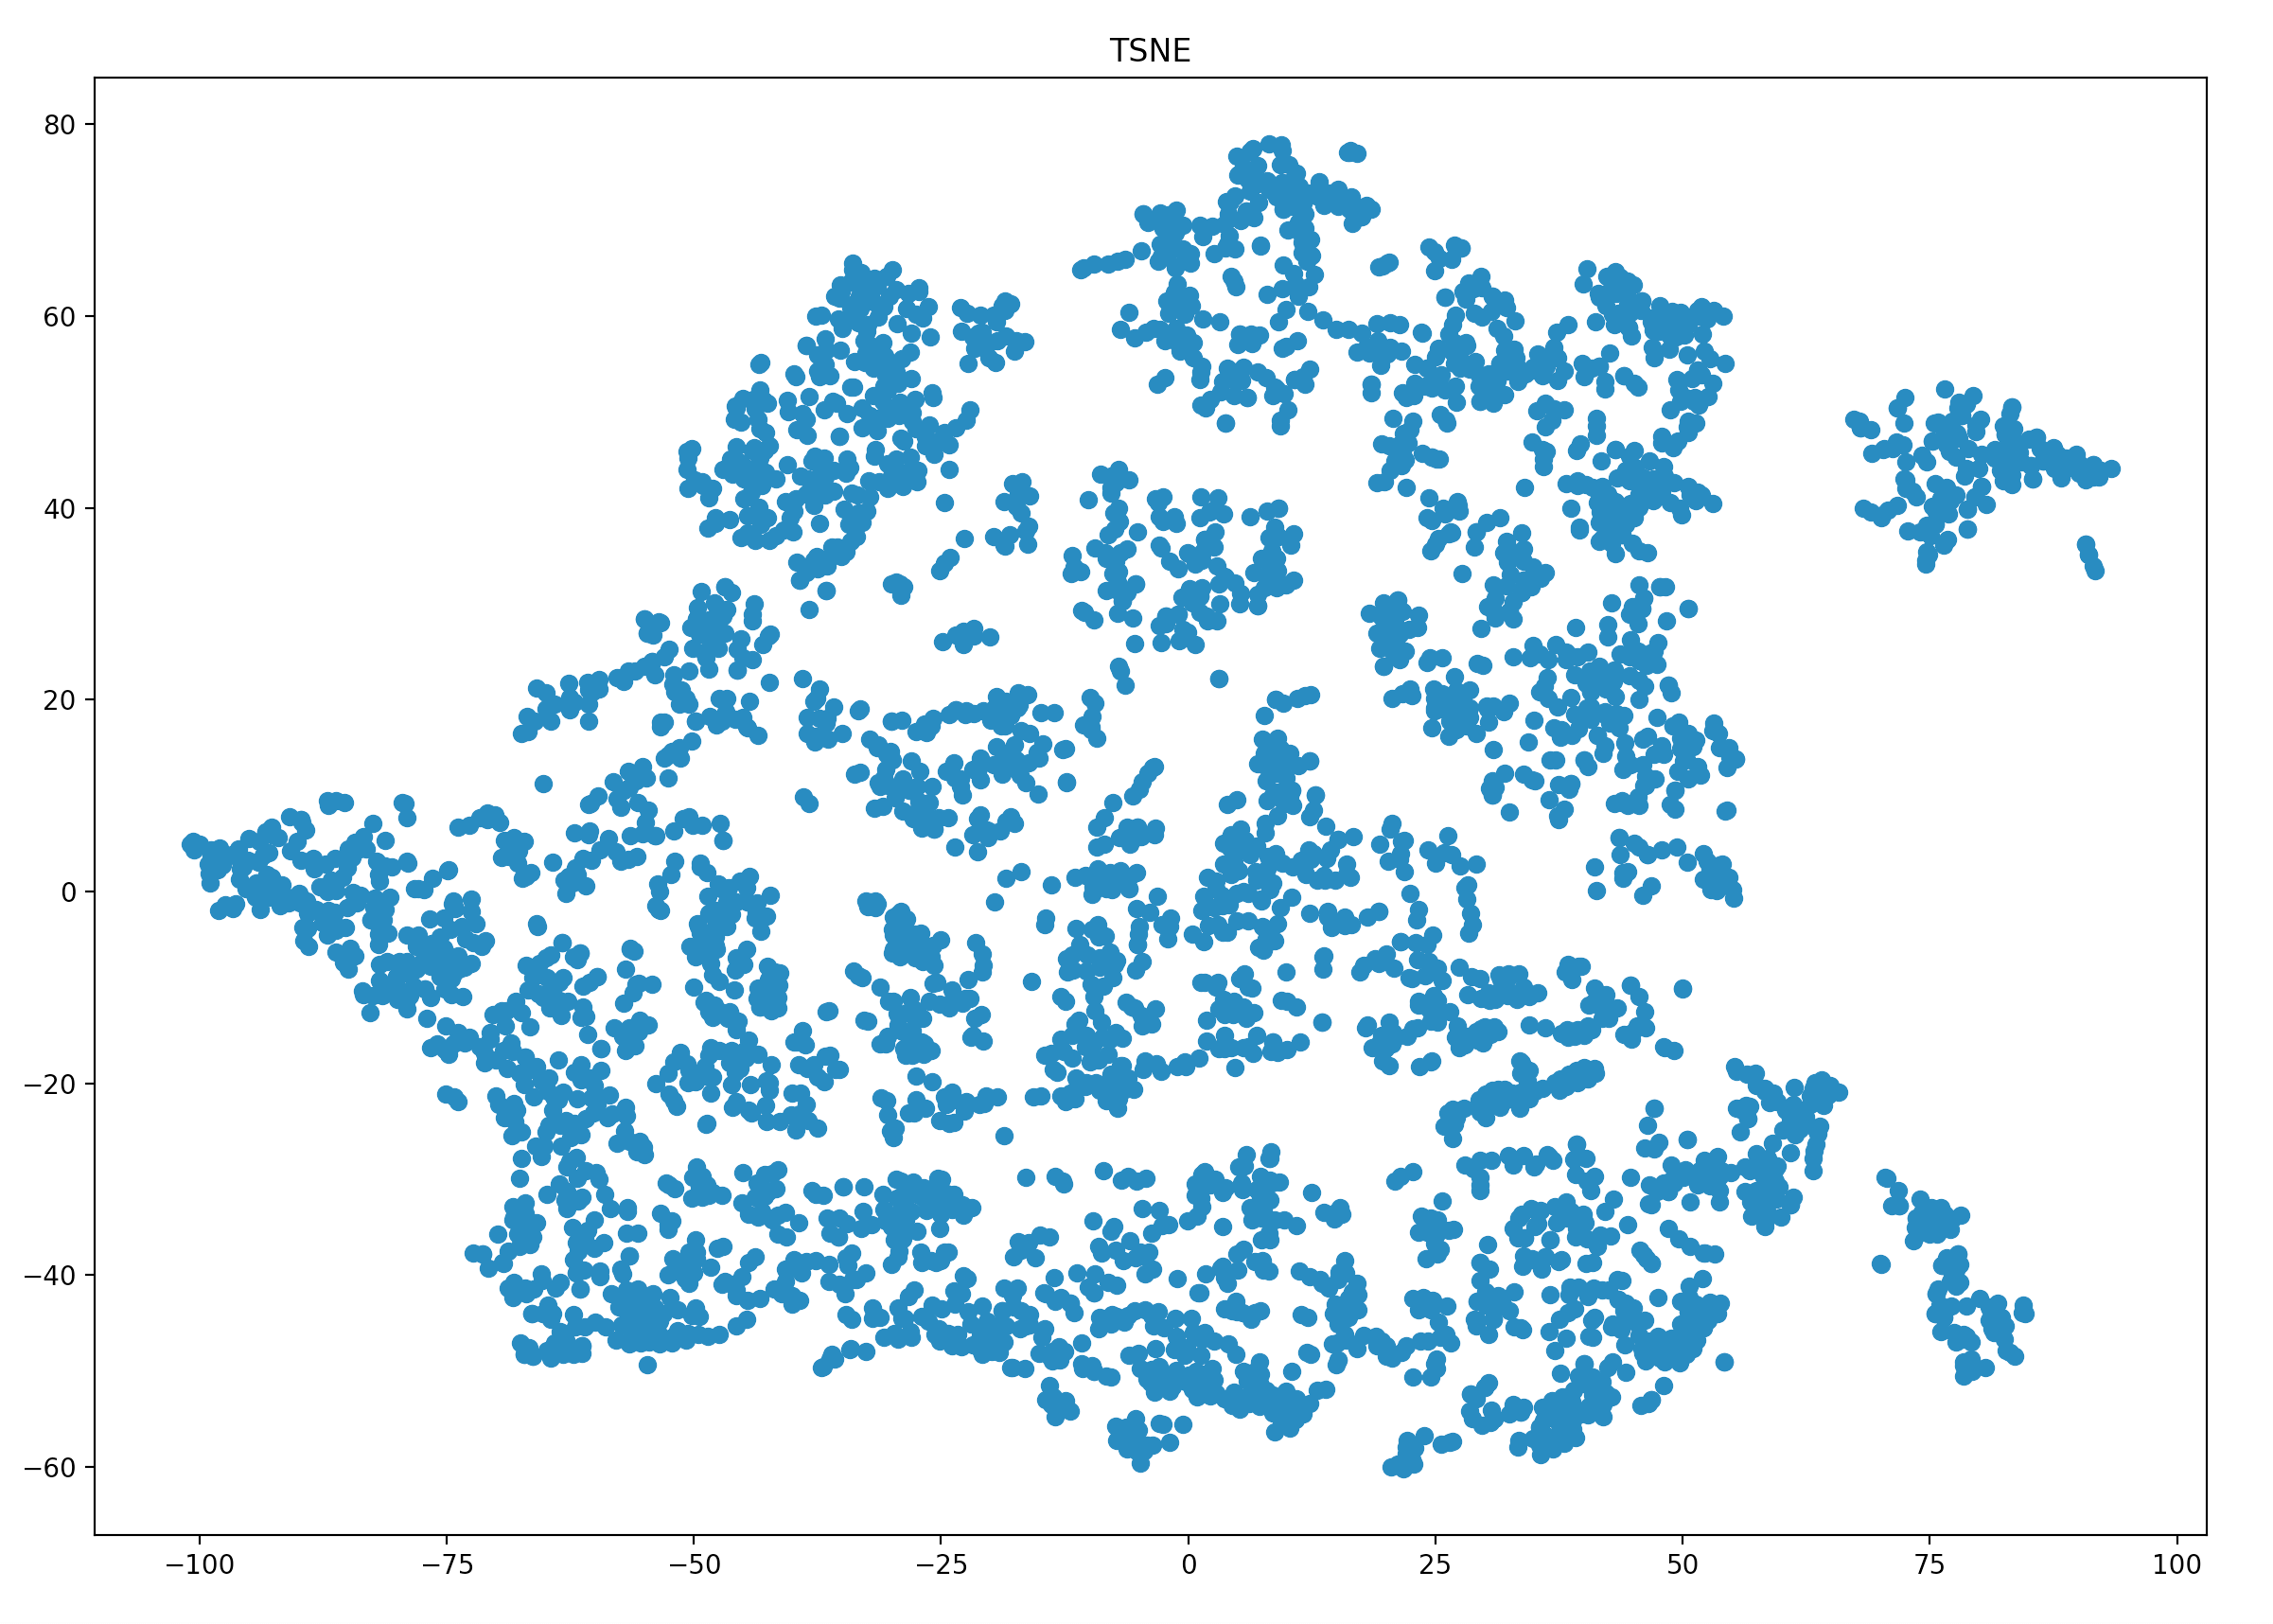
\includegraphics[width=0.9\textwidth]{./images/tsneParametersTest/learningRate/lr400-3hTSNE.png}
  \end{subfigure}%
  \begin{subfigure}{.5\textwidth}
    \centering
    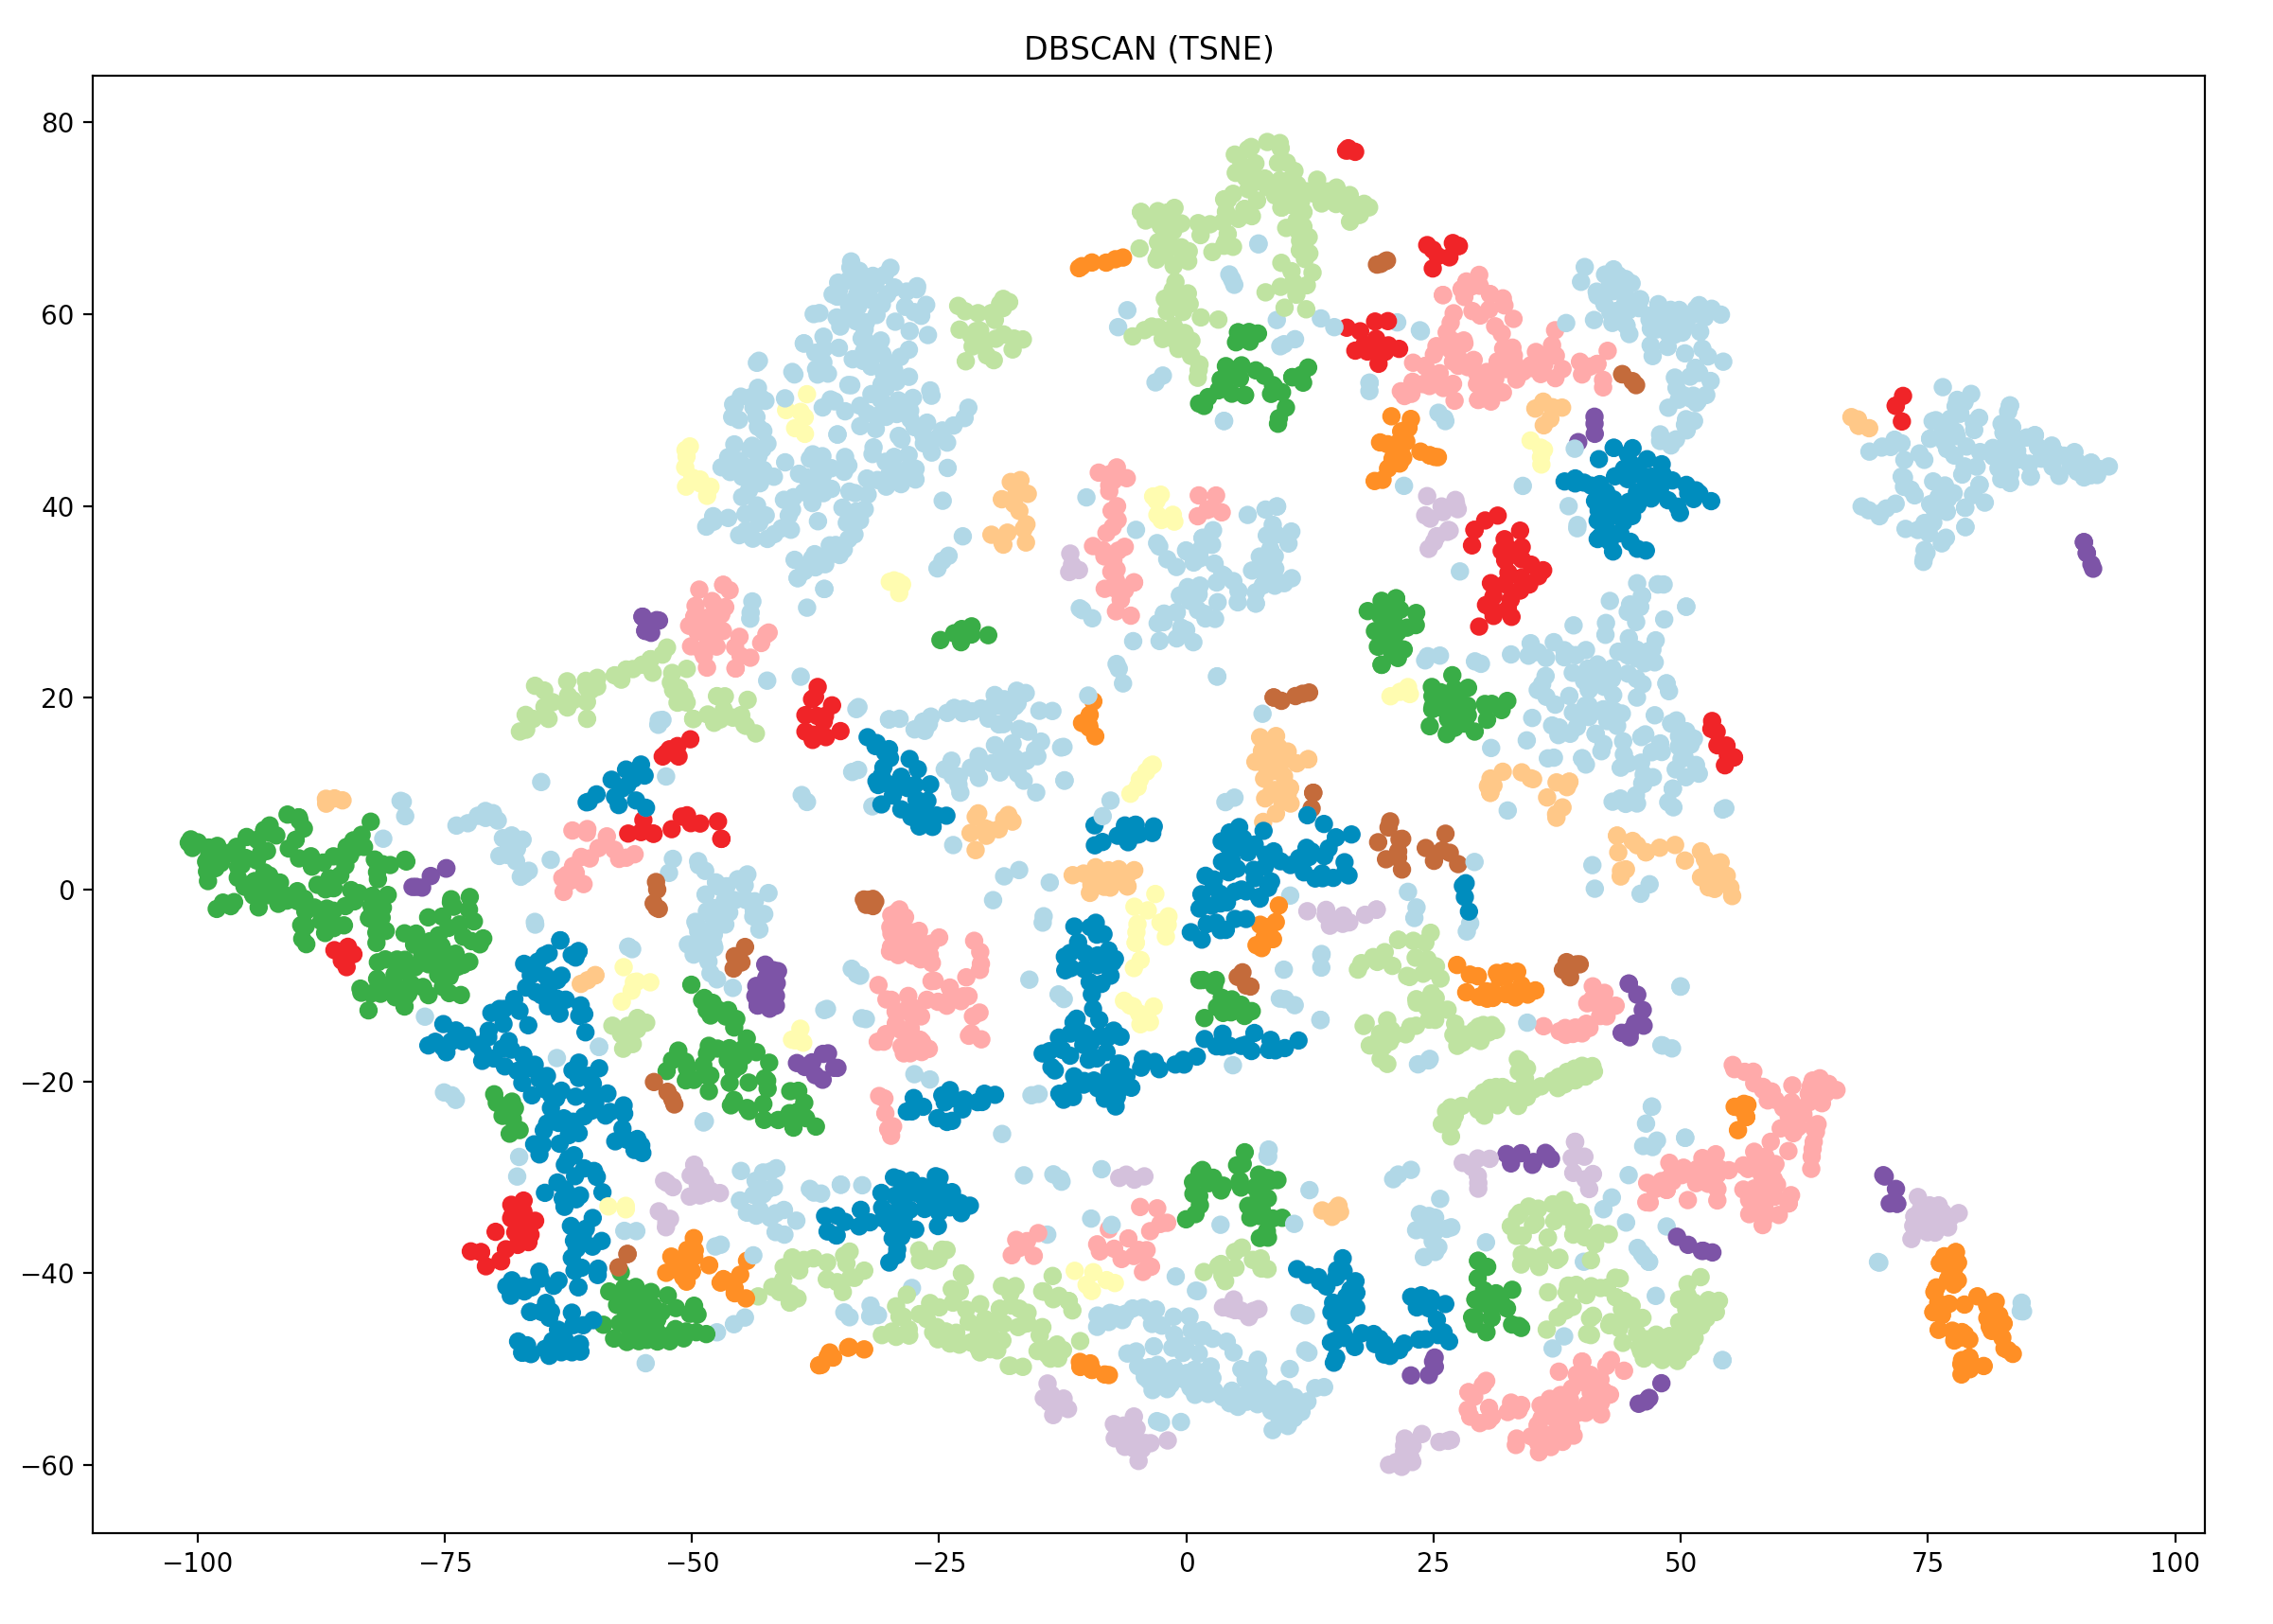
\includegraphics[width=0.9\textwidth]{./images/tsneParametersTest/learningRate/lr400-3hDBSCAN.png}
	\end{subfigure}
	\caption{\textbf{3h} data files, t-SNE calculated with the following parameters: perplexity=40, n\_iter=5000, \textbf{learning\_rate=400}}
  \label{figure:3hlr400TSNE}
\end{figure}


%------------------ LEARNING RATE 600: ------------------
\subsubsection{Learning Rate = 600}
% -- 1h, lr 600 --
\begin{figure}[H]
  \centering
  \begin{subfigure}{.5\textwidth}
    \centering
    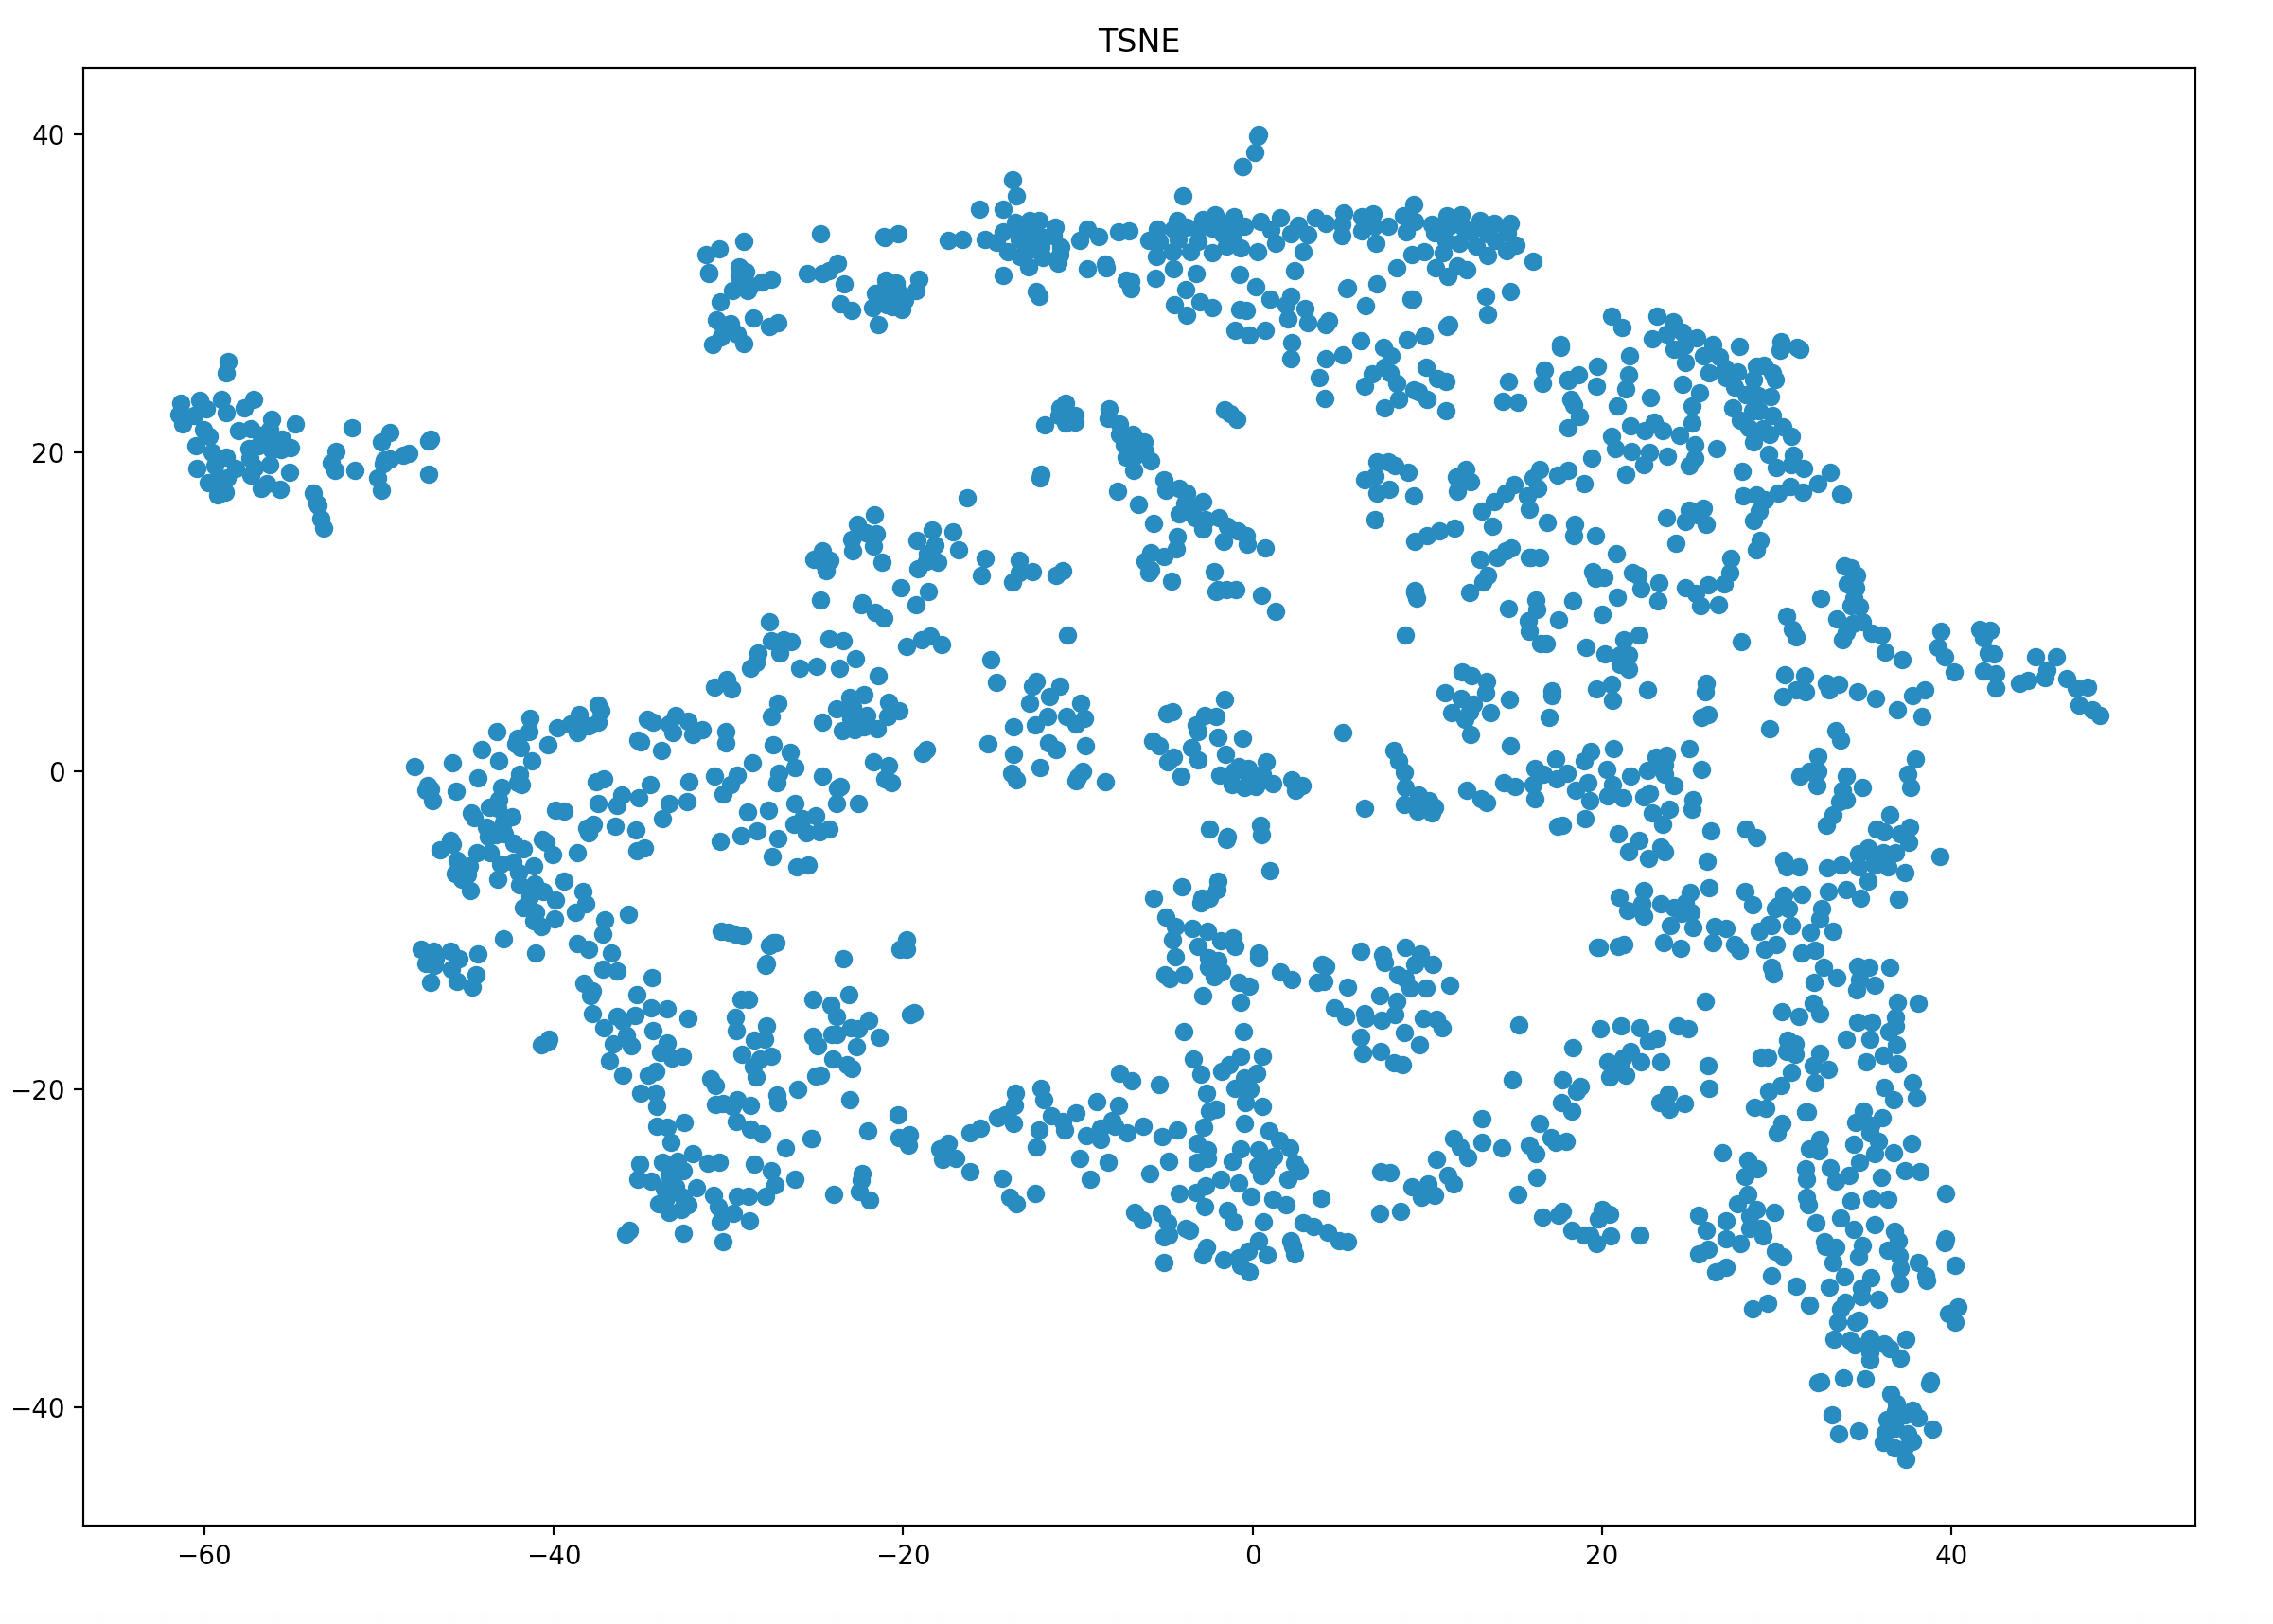
\includegraphics[width=0.9\textwidth]{./images/tsneParametersTest/learningRate/lr600-1hTSNE.png}
  \end{subfigure}%
  \begin{subfigure}{.5\textwidth}
    \centering
    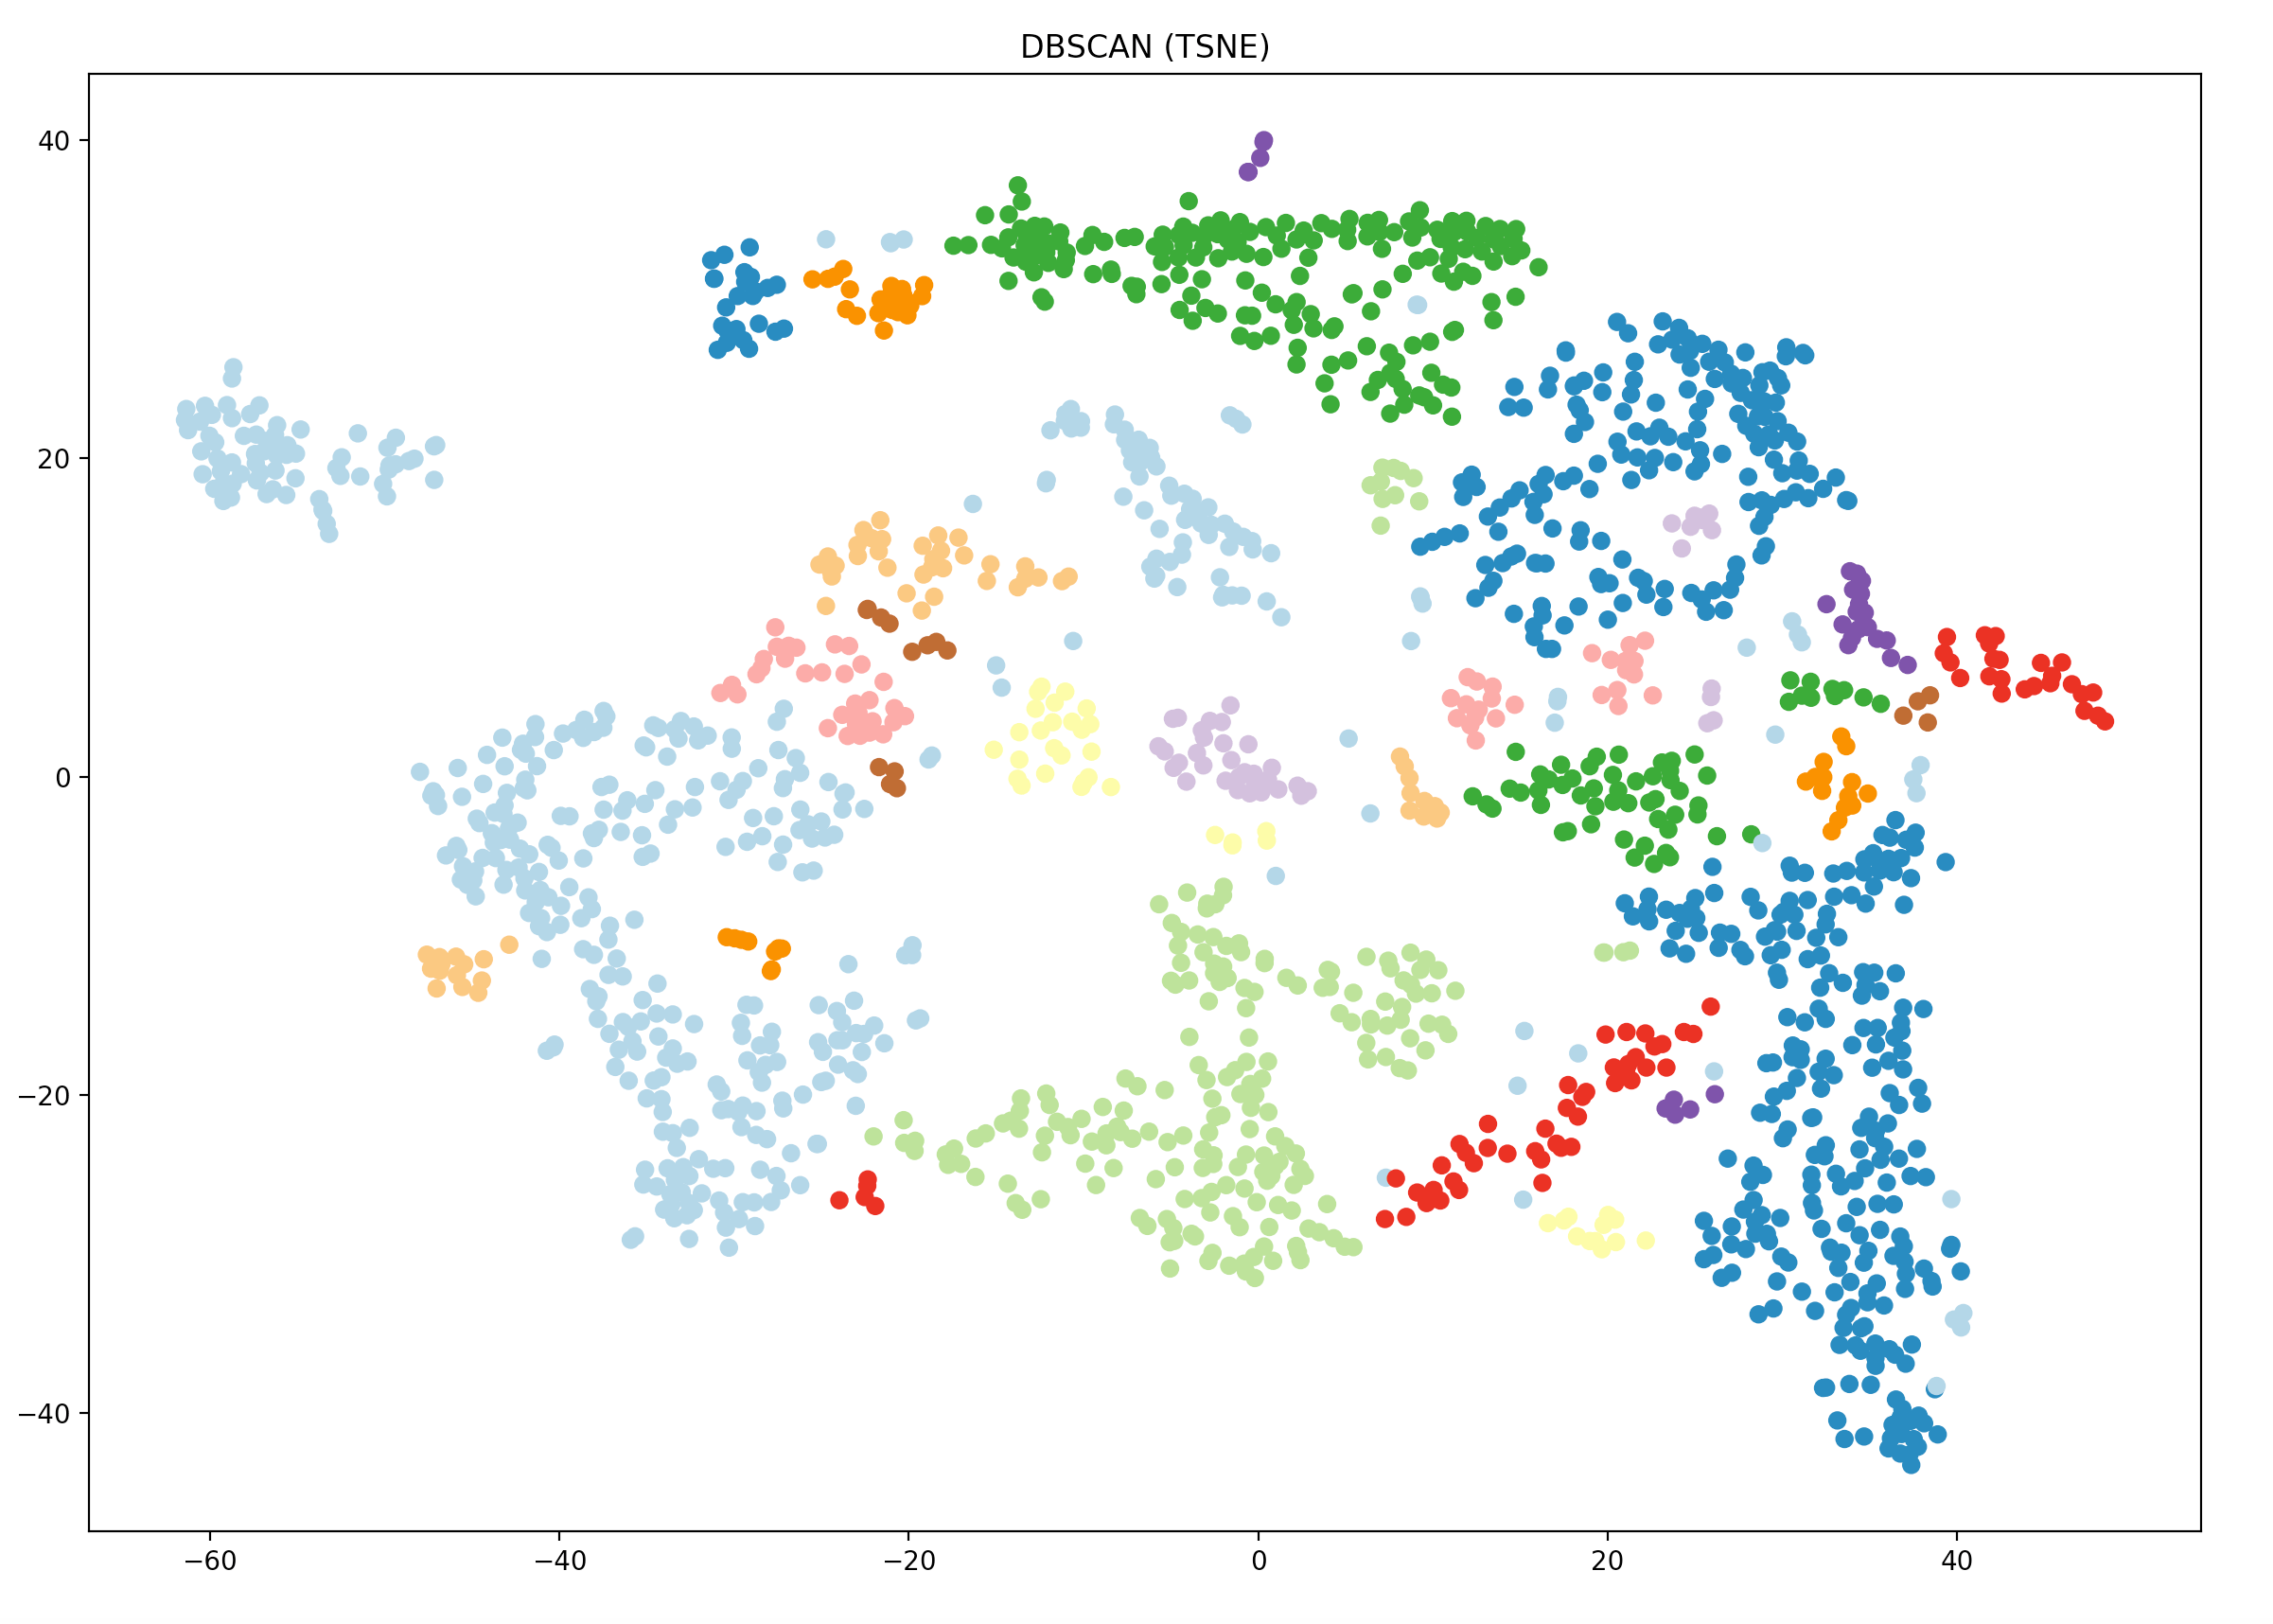
\includegraphics[width=0.9\textwidth]{./images/tsneParametersTest/learningRate/lr600-1hDBSCAN.png}
  \end{subfigure}
	\caption{\textbf{1h} data files, t-SNE calculated with the following parameters: perplexity=40, n\_iter=5000, \textbf{learning\_rate=600}}
	\label{figure:1hlr600TSNE}
\end{figure}

% -- 3h, lr 600 --
\begin{figure}[H]
	\centering
	
  \centering
	\begin{subfigure}{.5\textwidth}
    \centering
    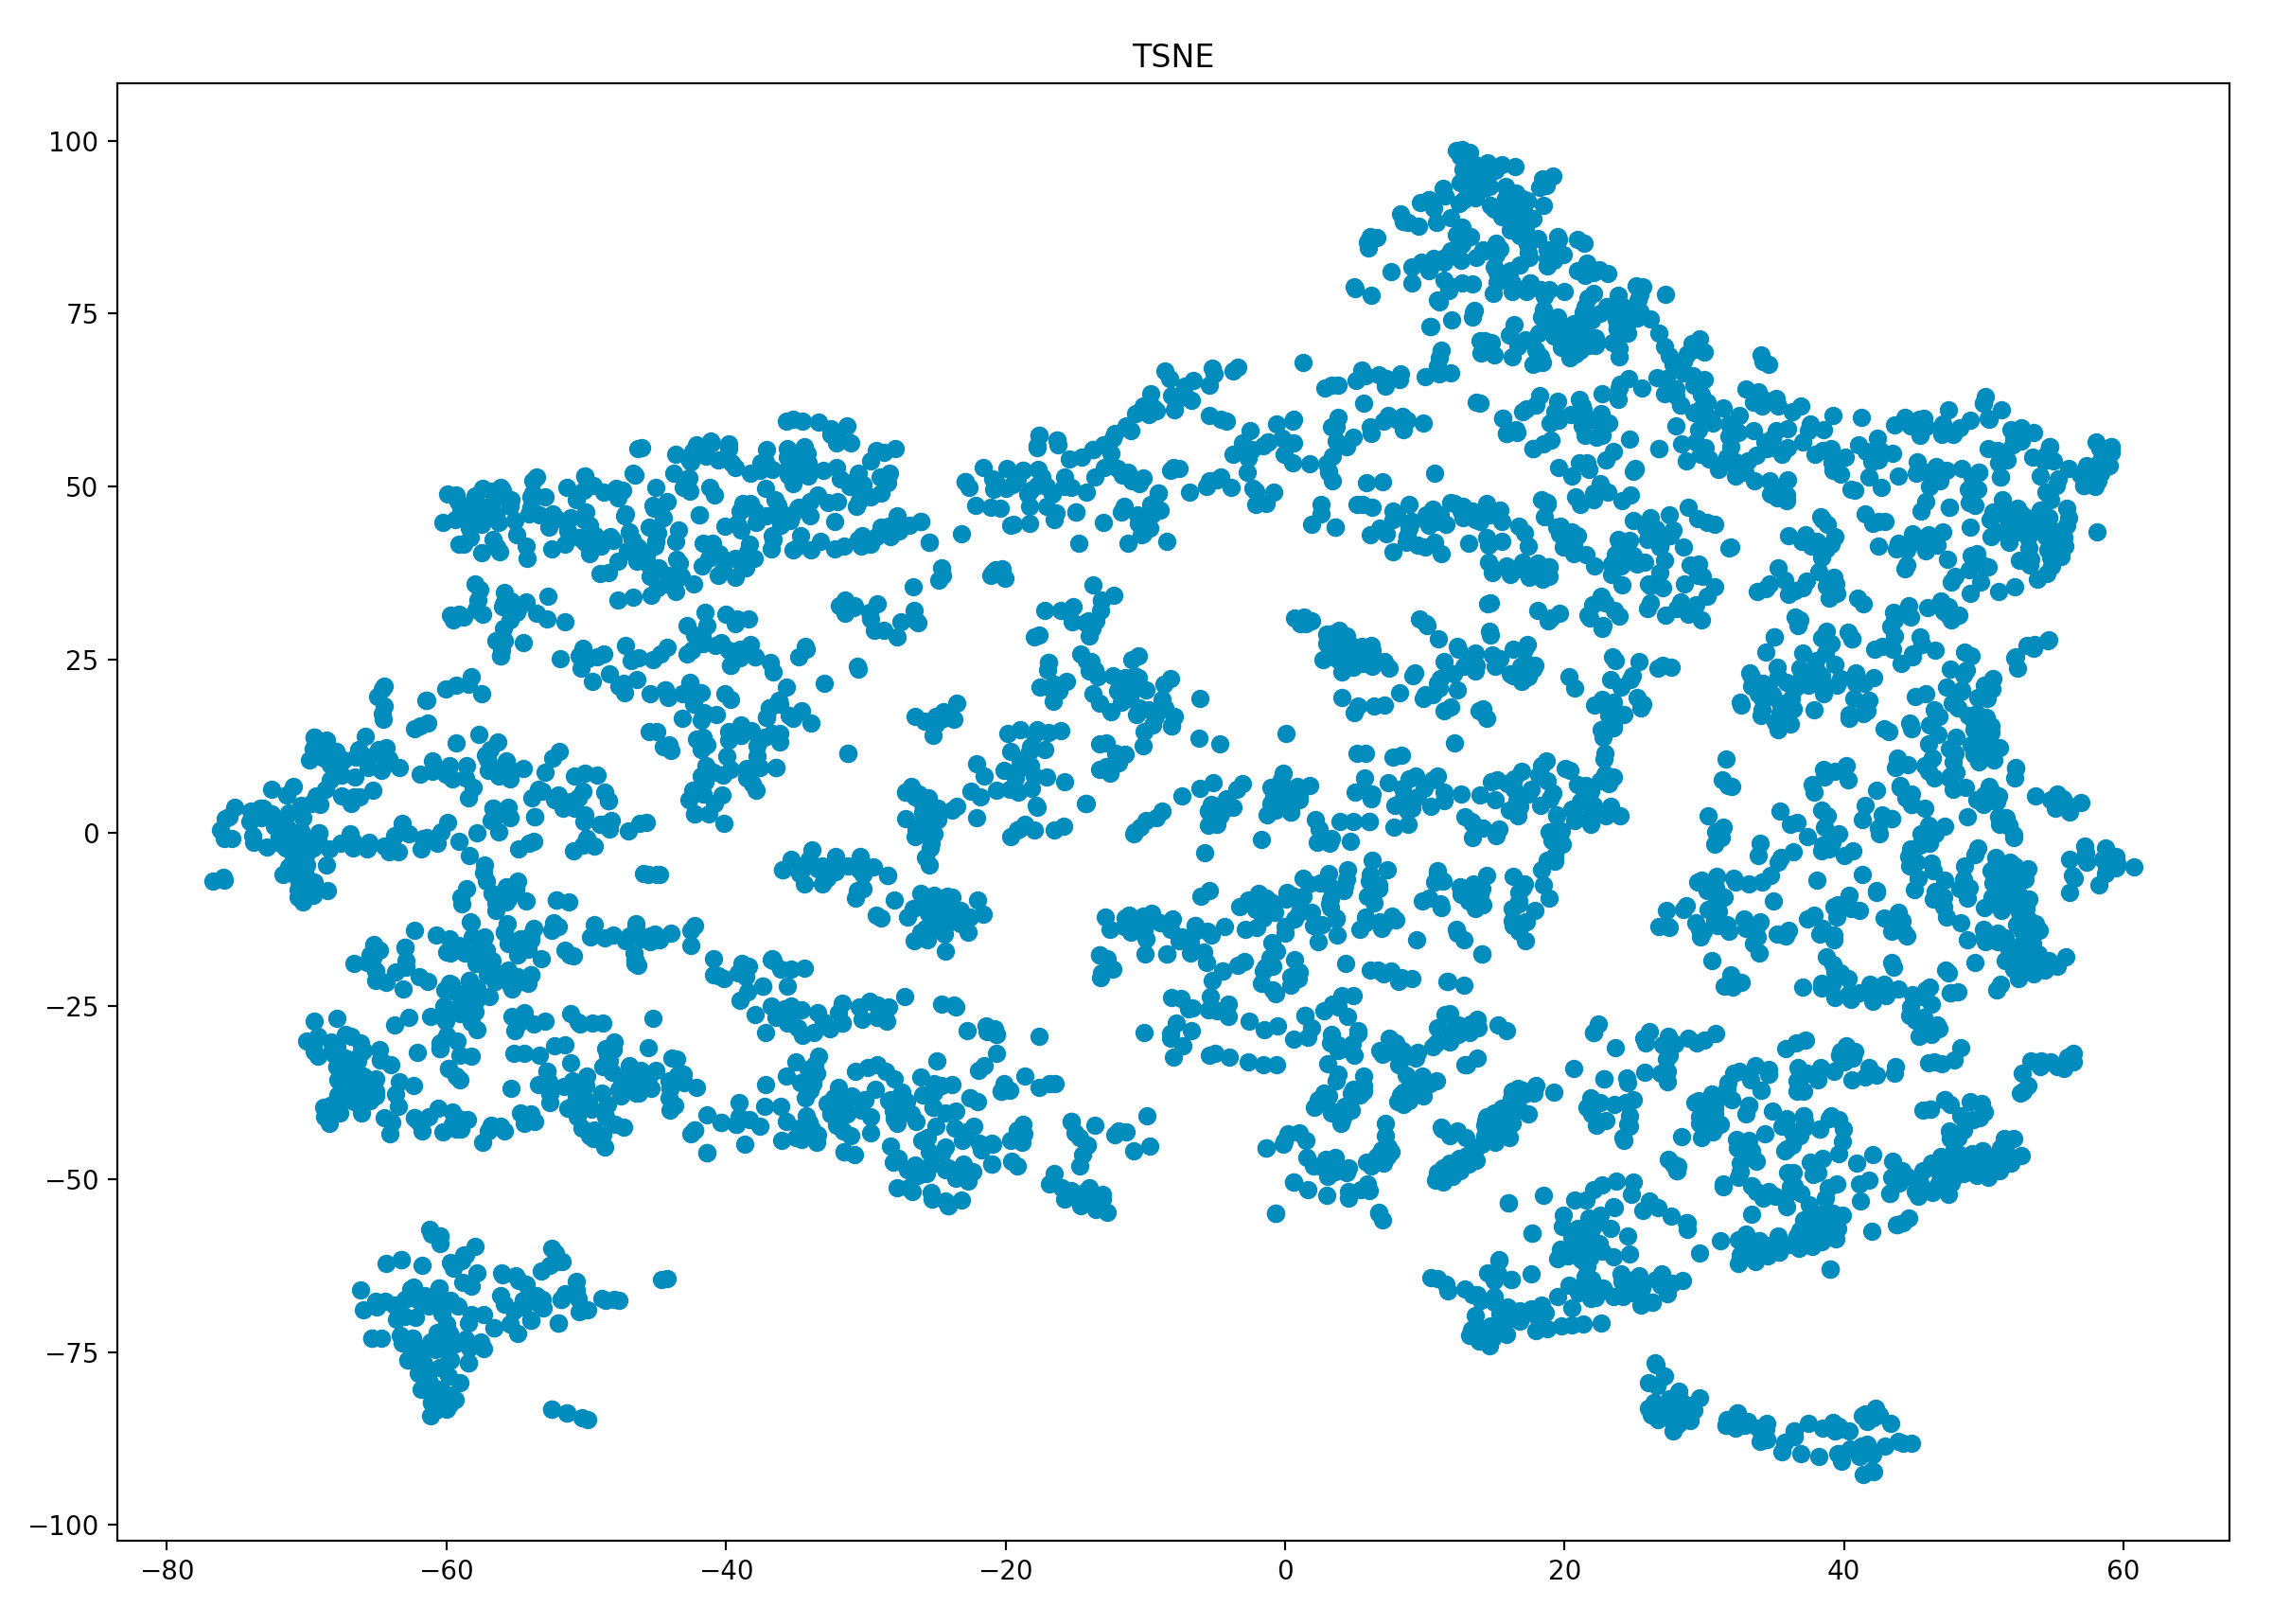
\includegraphics[width=0.9\textwidth]{./images/tsneParametersTest/learningRate/lr600-3hTSNE.png}
  \end{subfigure}%
  \begin{subfigure}{.5\textwidth}
    \centering
    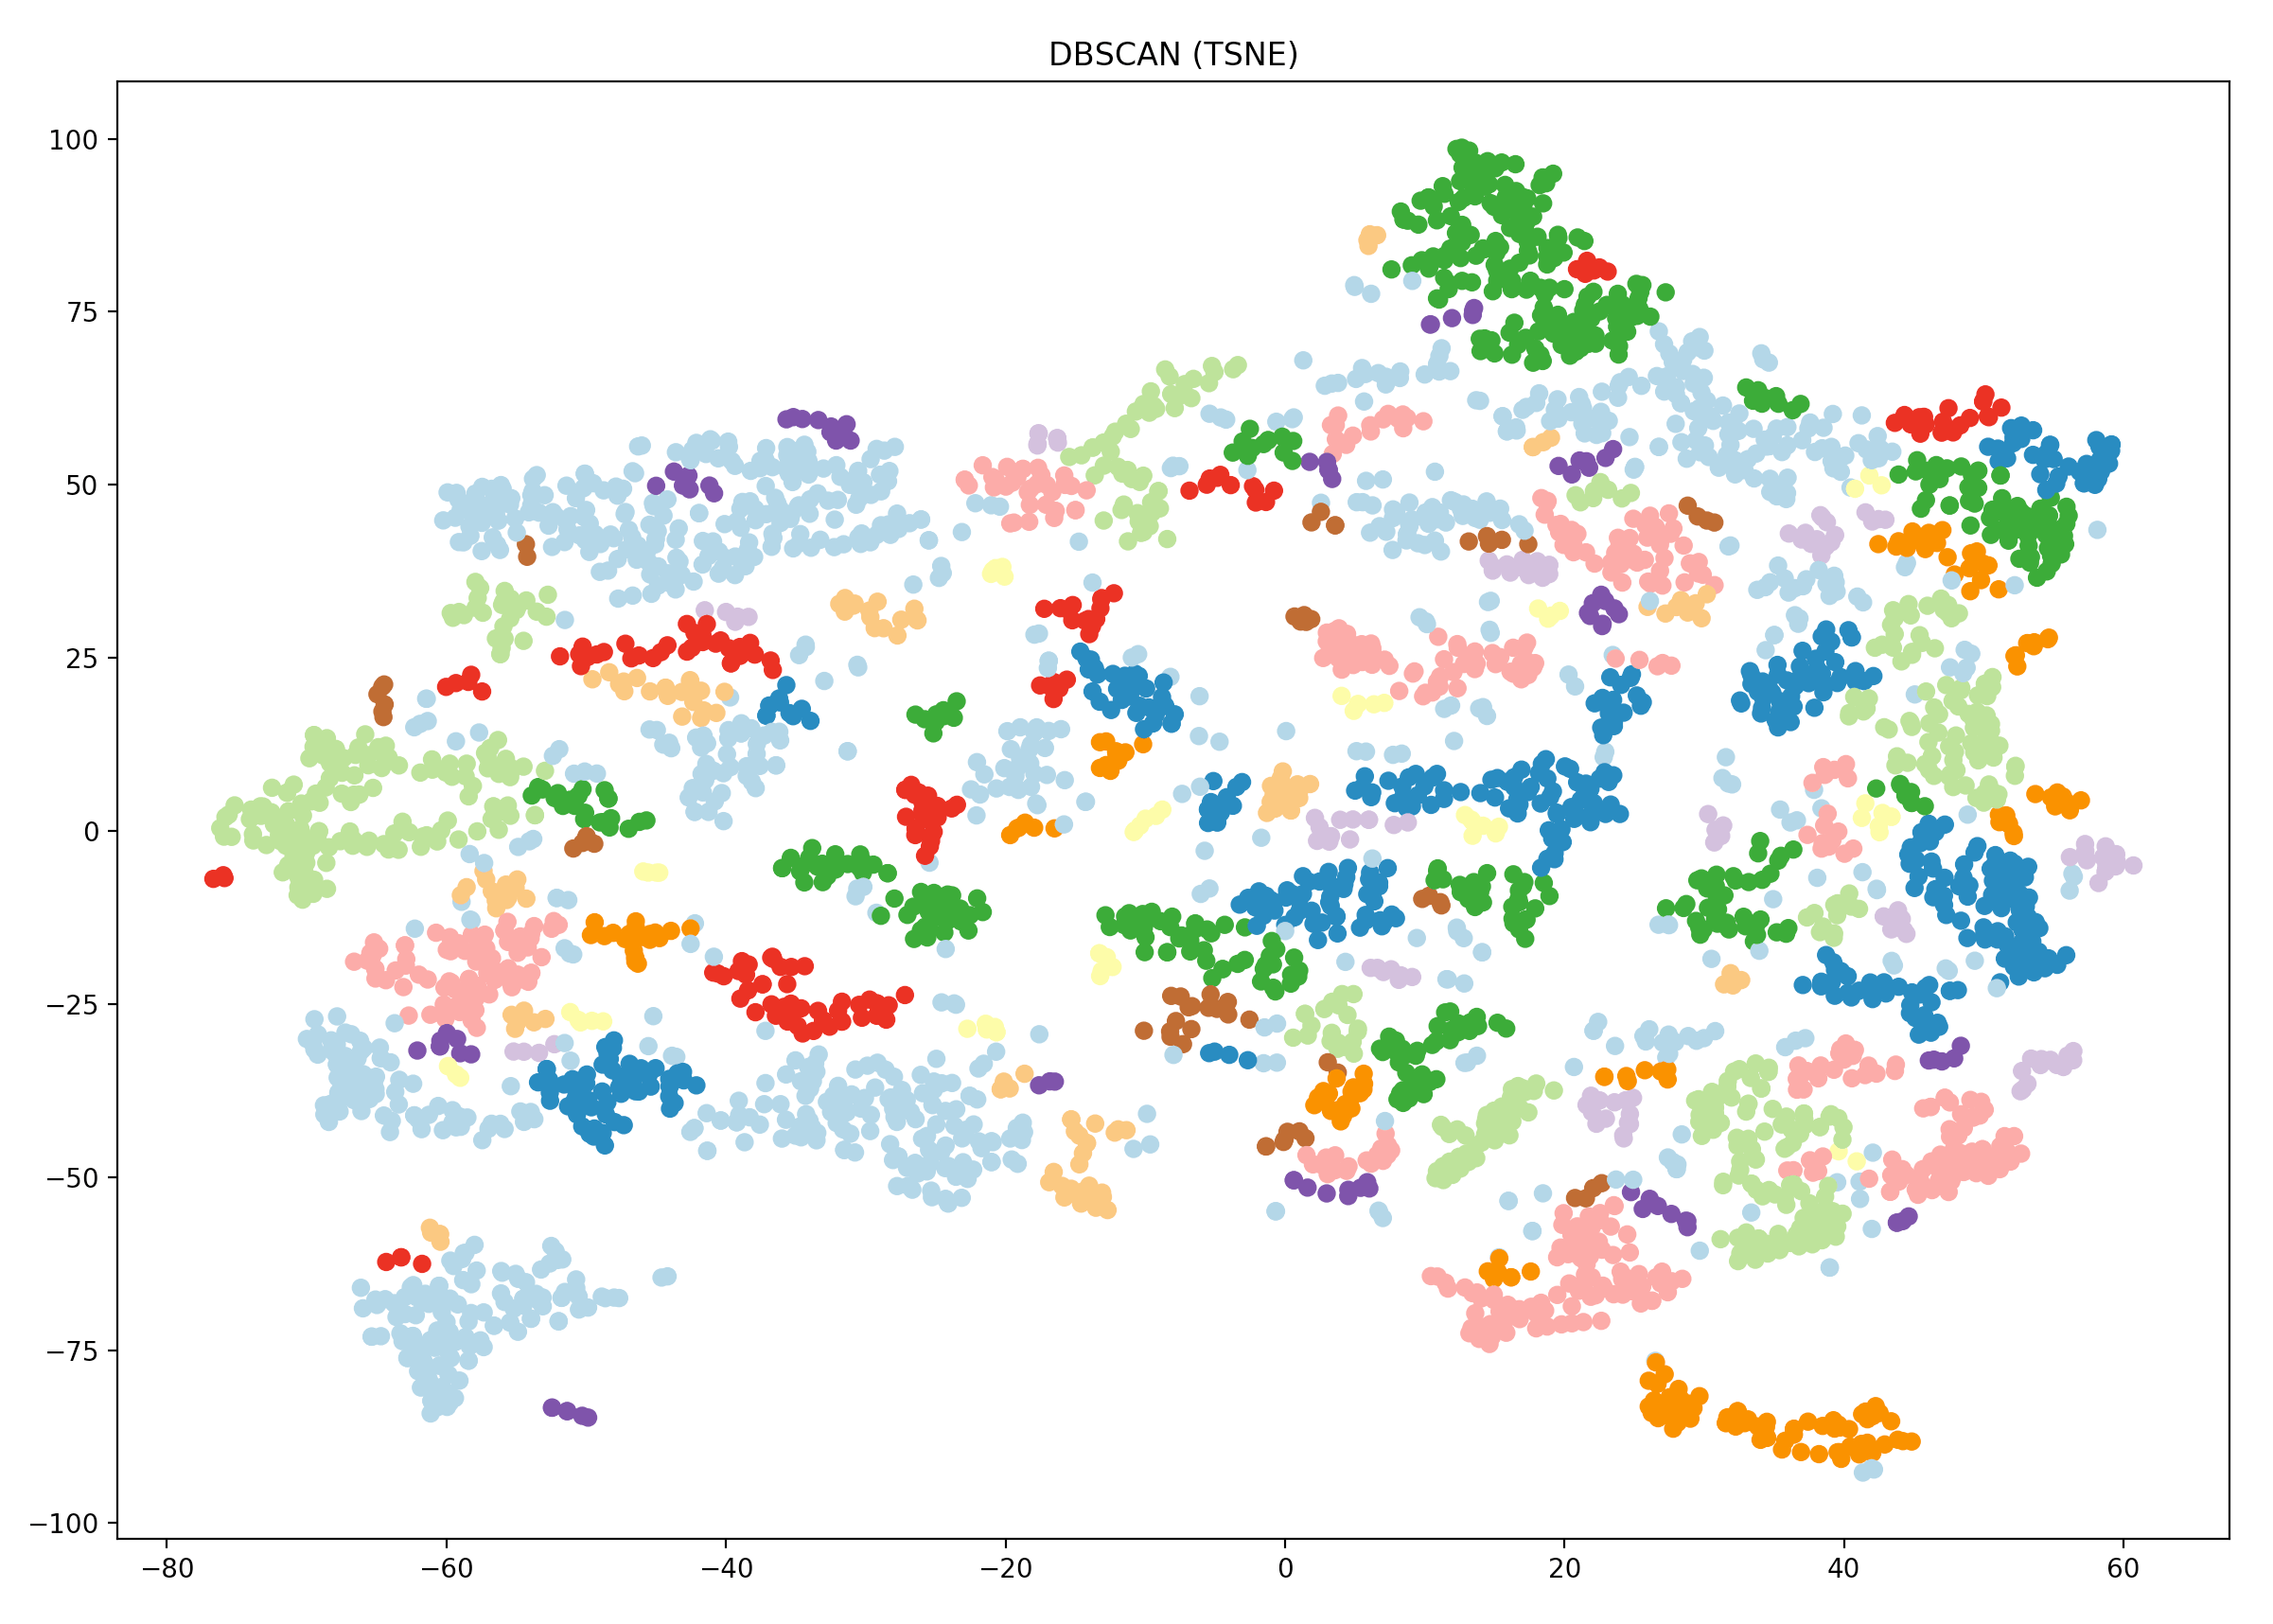
\includegraphics[width=0.9\textwidth]{./images/tsneParametersTest/learningRate/lr600-3hDBSCAN.png}
	\end{subfigure}
	\caption{\textbf{3h} data files, t-SNE calculated with the following parameters: perplexity=40, n\_iter=5000, \textbf{learning\_rate=600}}
  \label{figure:3hlr600TSNE}
\end{figure}




%------------------ LEARNING RATE 800: ------------------
\subsubsection{Learning Rate = 800}
% -- 1h, lr 800 --
\begin{figure}[H]
  \centering
  \begin{subfigure}{.5\textwidth}
    \centering
    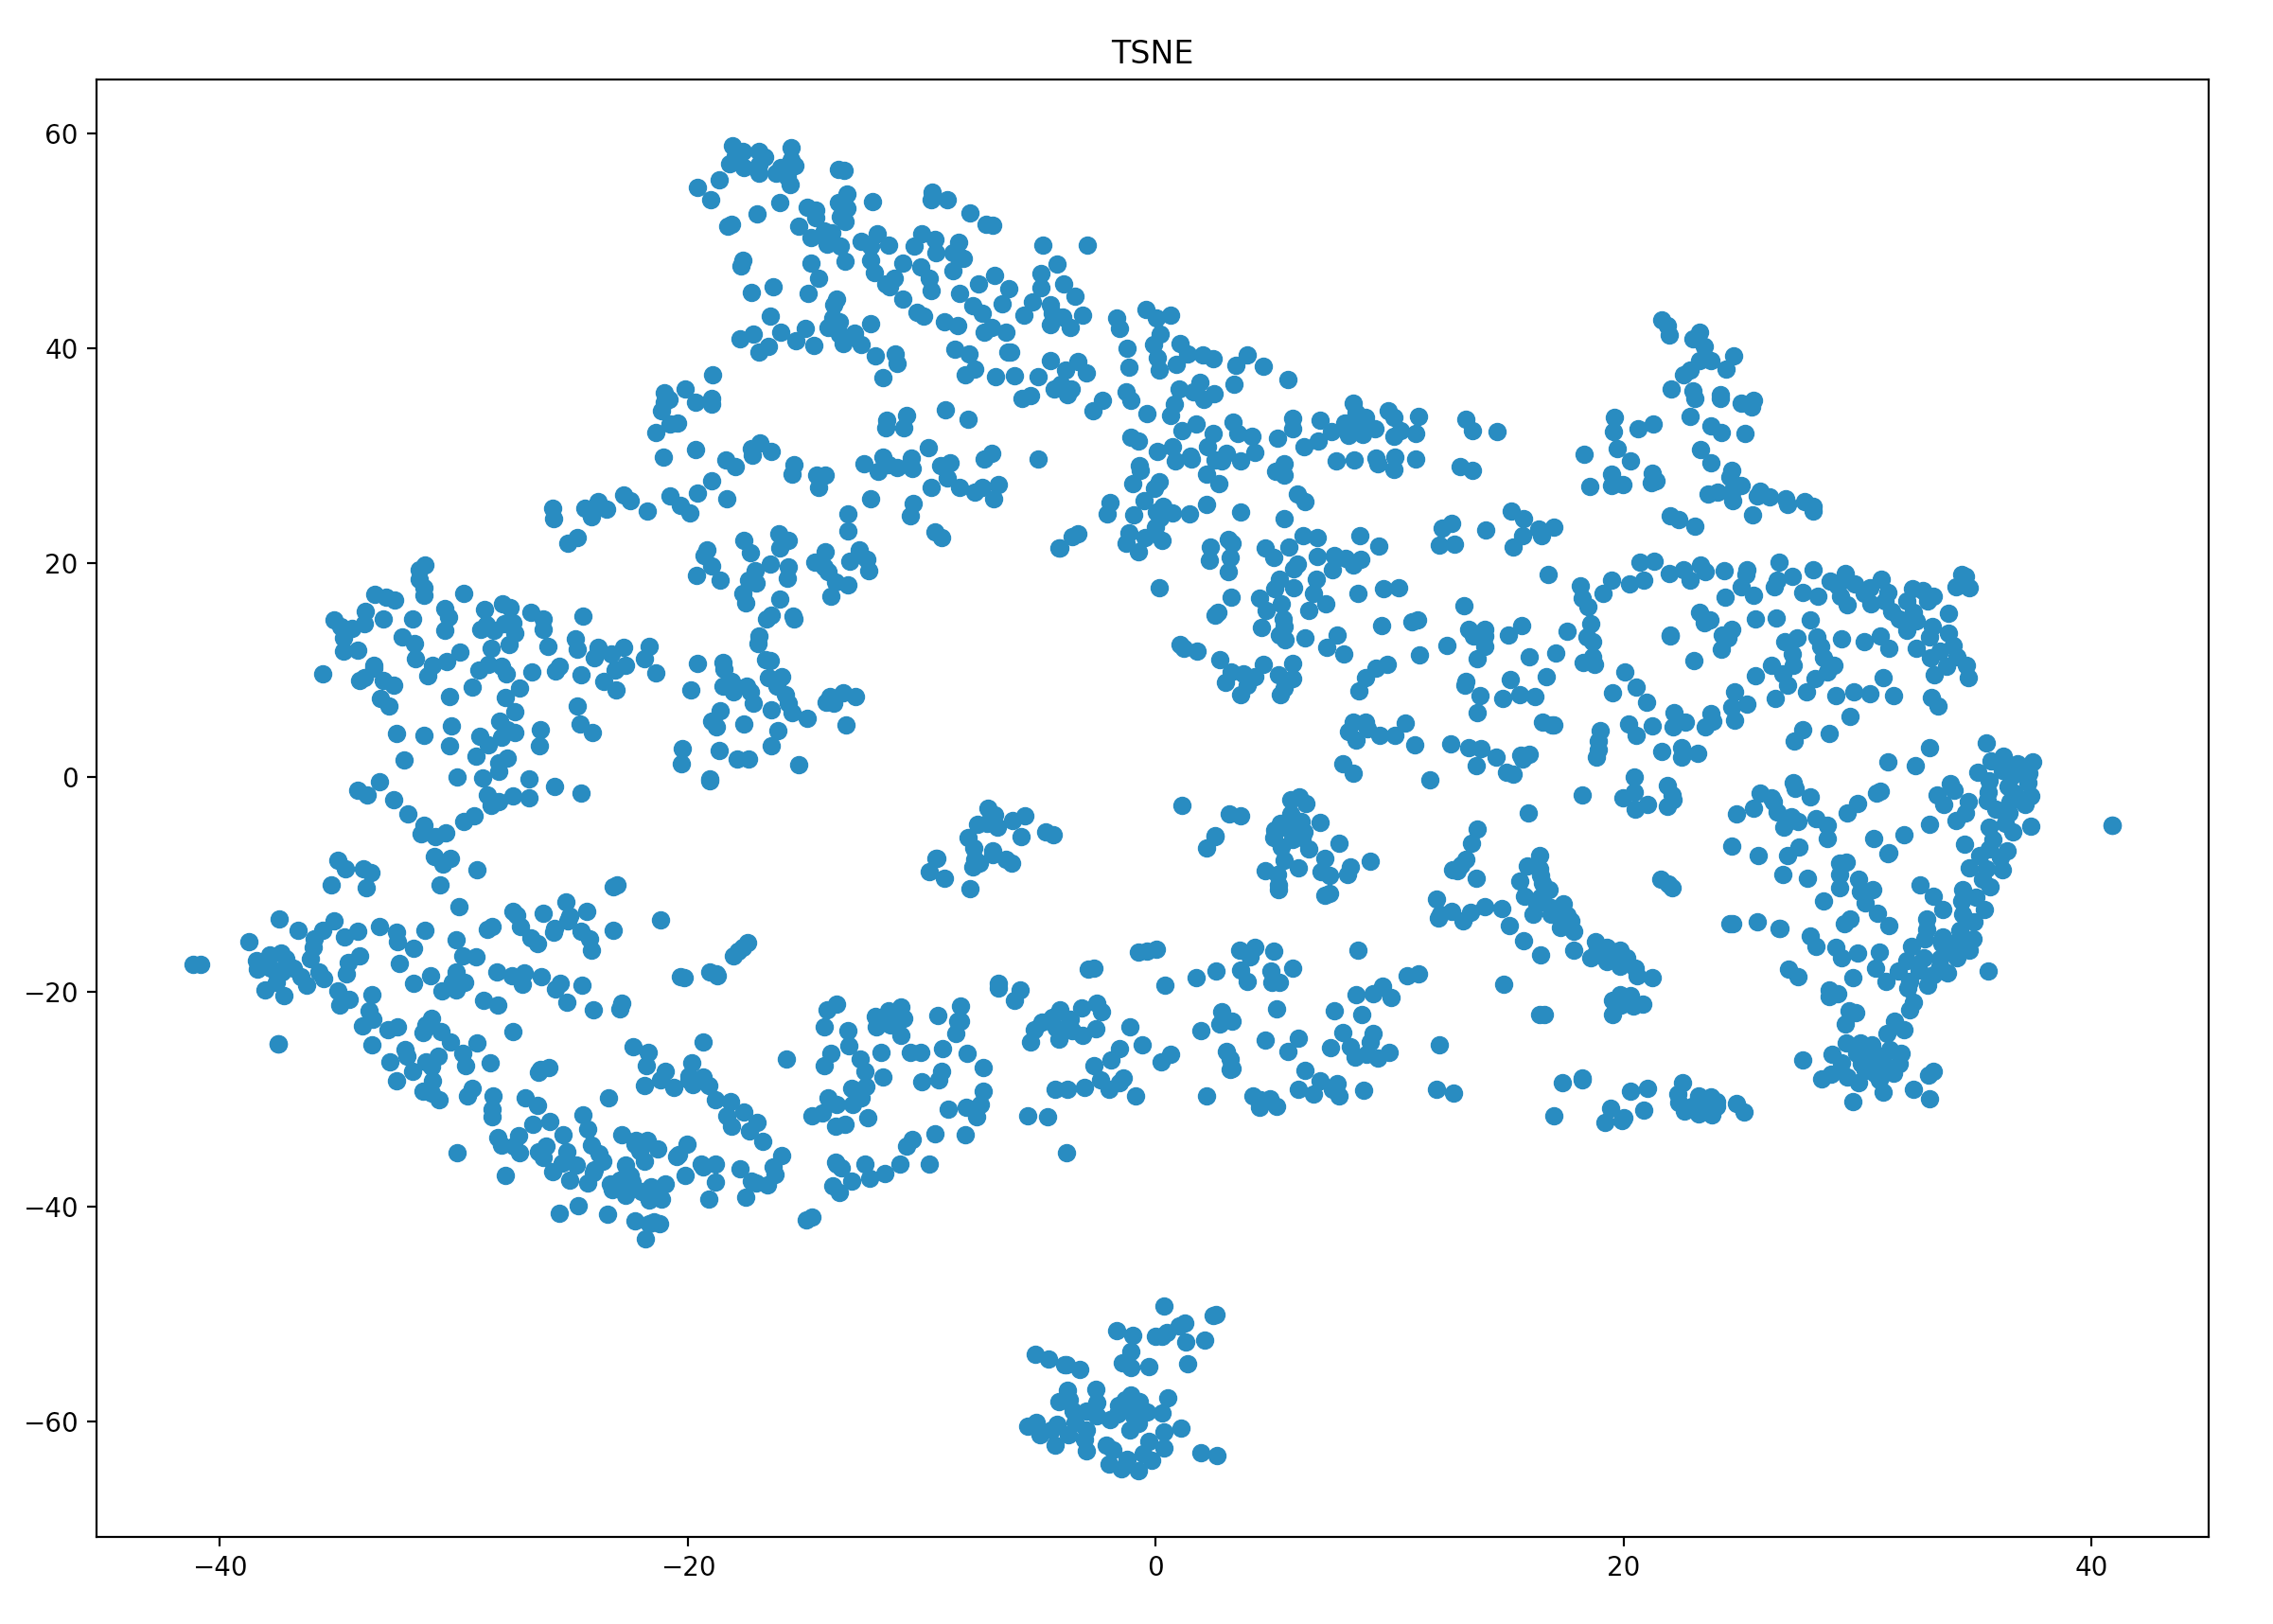
\includegraphics[width=0.9\textwidth]{./images/tsneParametersTest/learningRate/lr800-1hTSNE.png}
  \end{subfigure}%
  \begin{subfigure}{.5\textwidth}
    \centering
    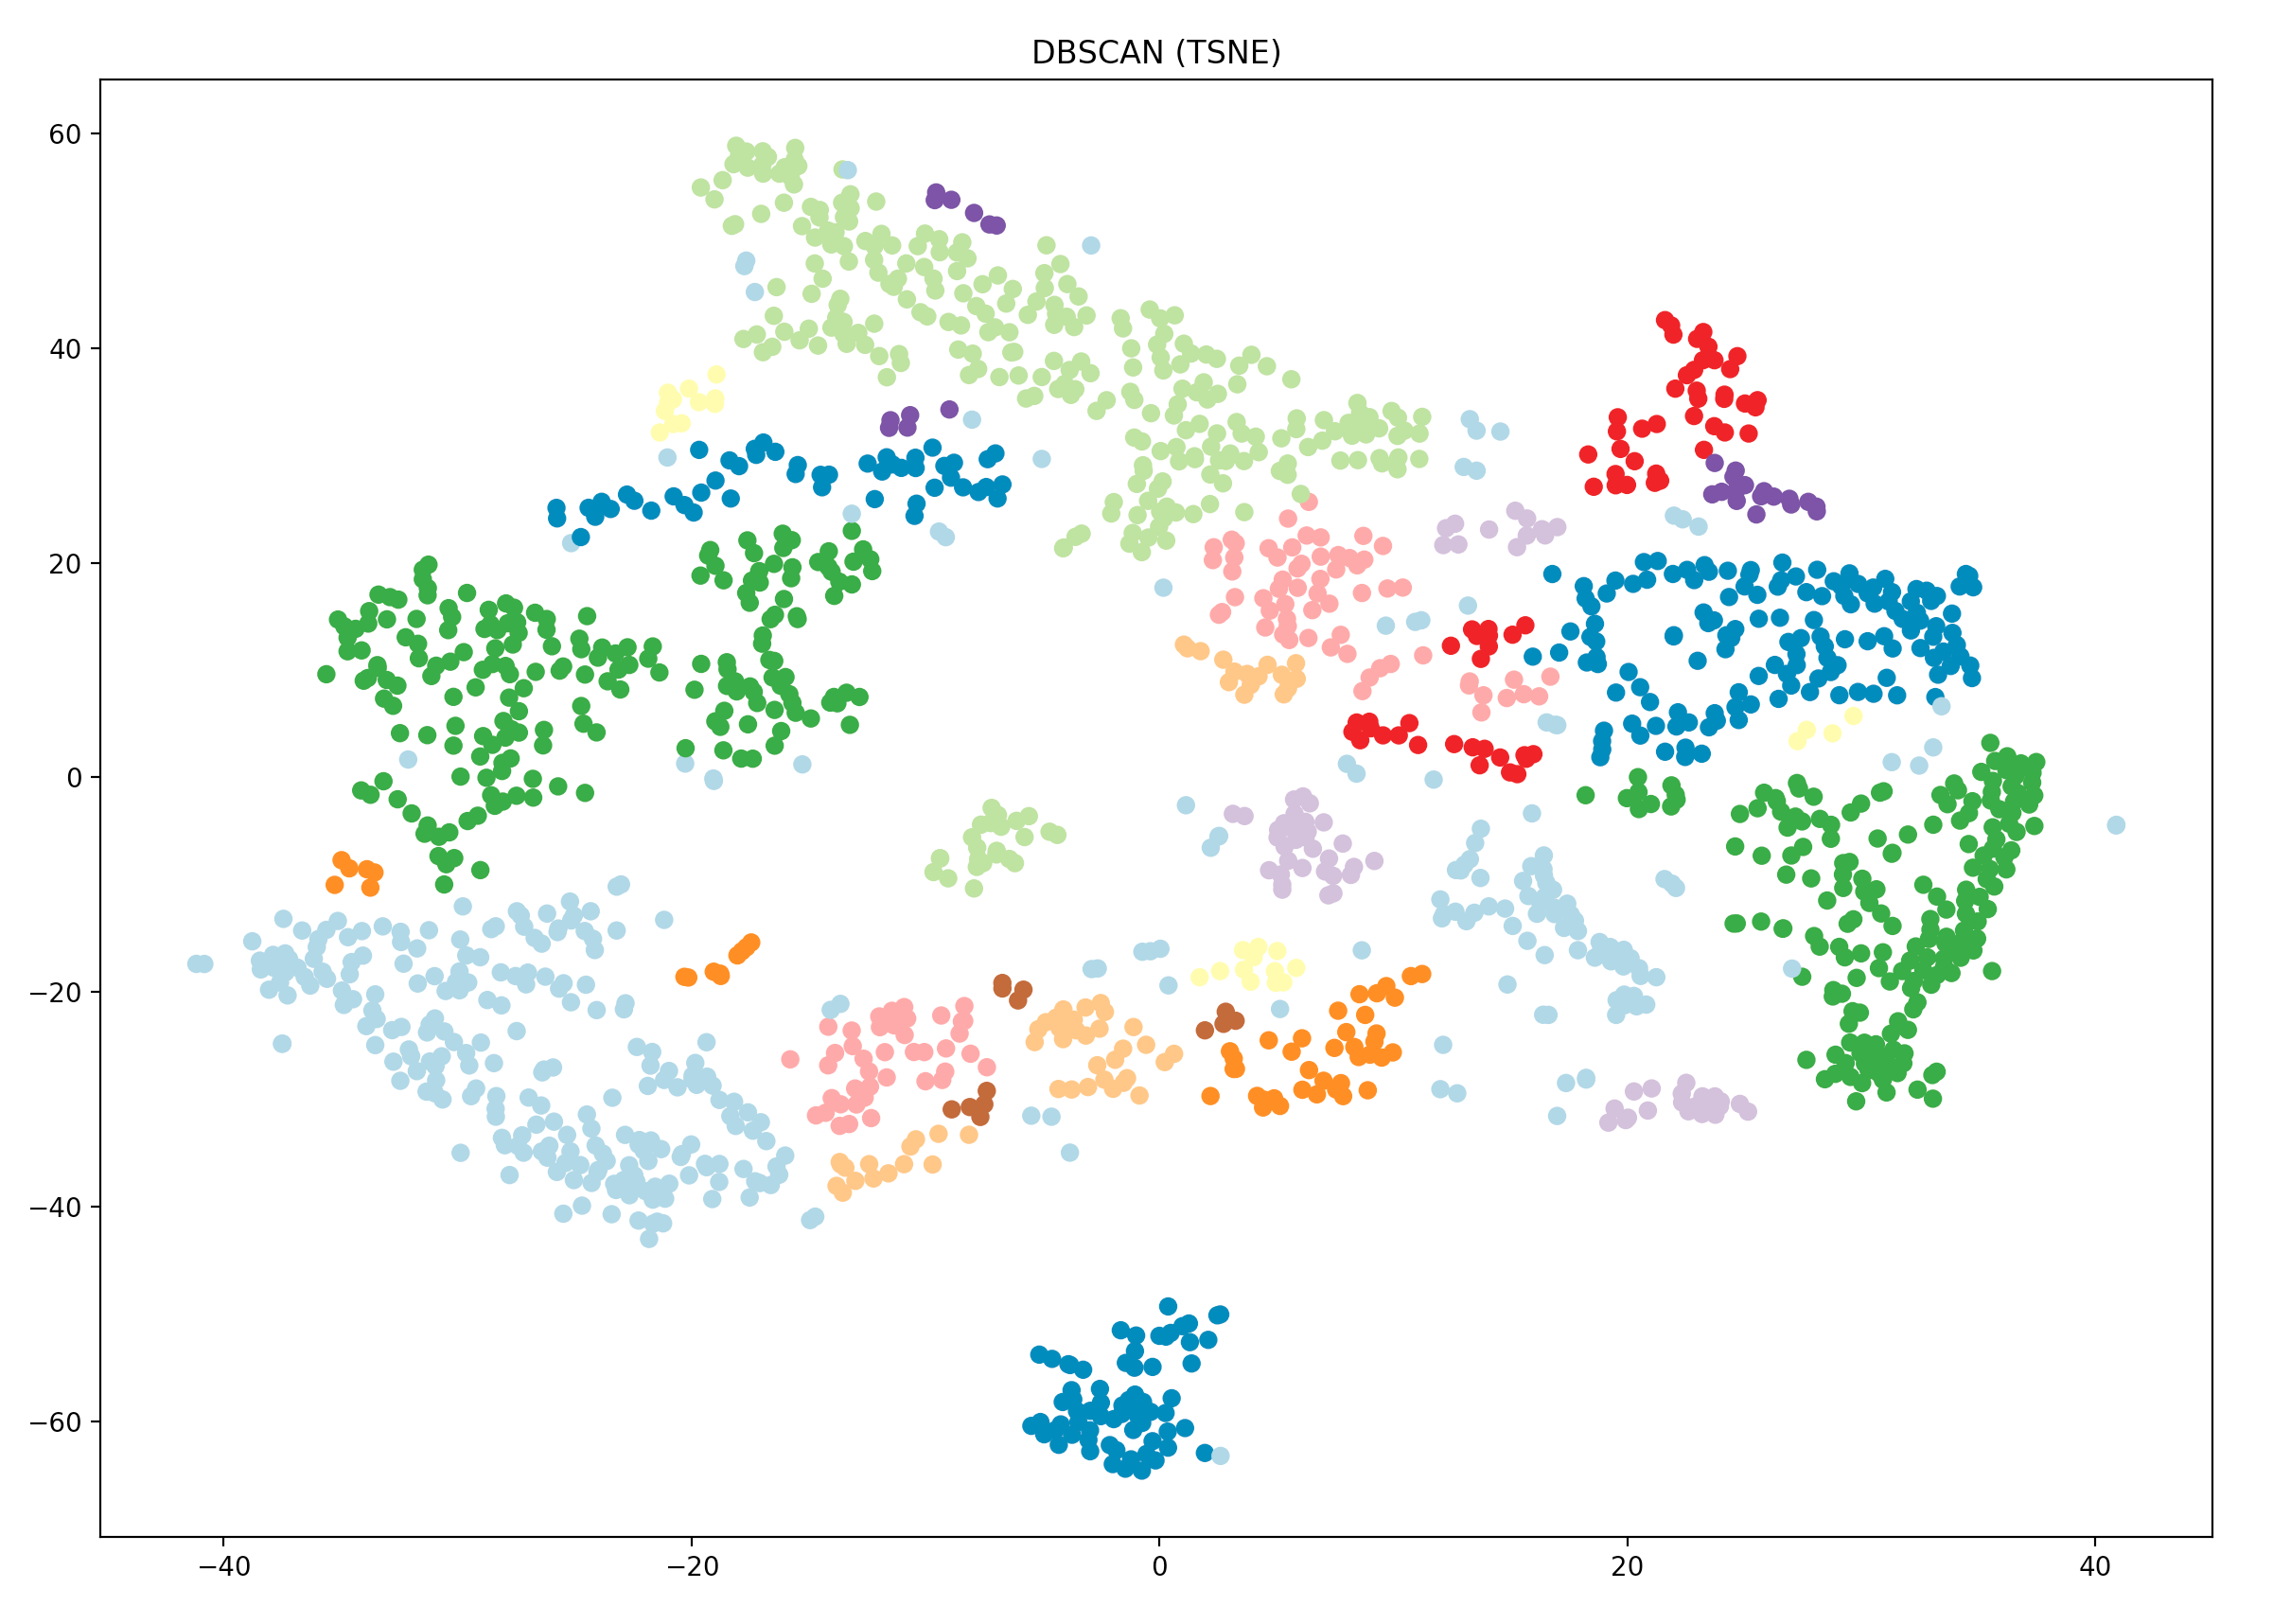
\includegraphics[width=0.9\textwidth]{./images/tsneParametersTest/learningRate/lr800-1hDBSCAN.png}
  \end{subfigure}
	\caption{\textbf{1h} data files, t-SNE calculated with the following parameters: perplexity=40, n\_iter=5000, \textbf{learning\_rate=800}}
	\label{figure:1hlr800TSNE}
\end{figure}

% -- 3h, lr 800 --
\begin{figure}[H]
	\centering
	
  \centering
	\begin{subfigure}{.5\textwidth}
    \centering
    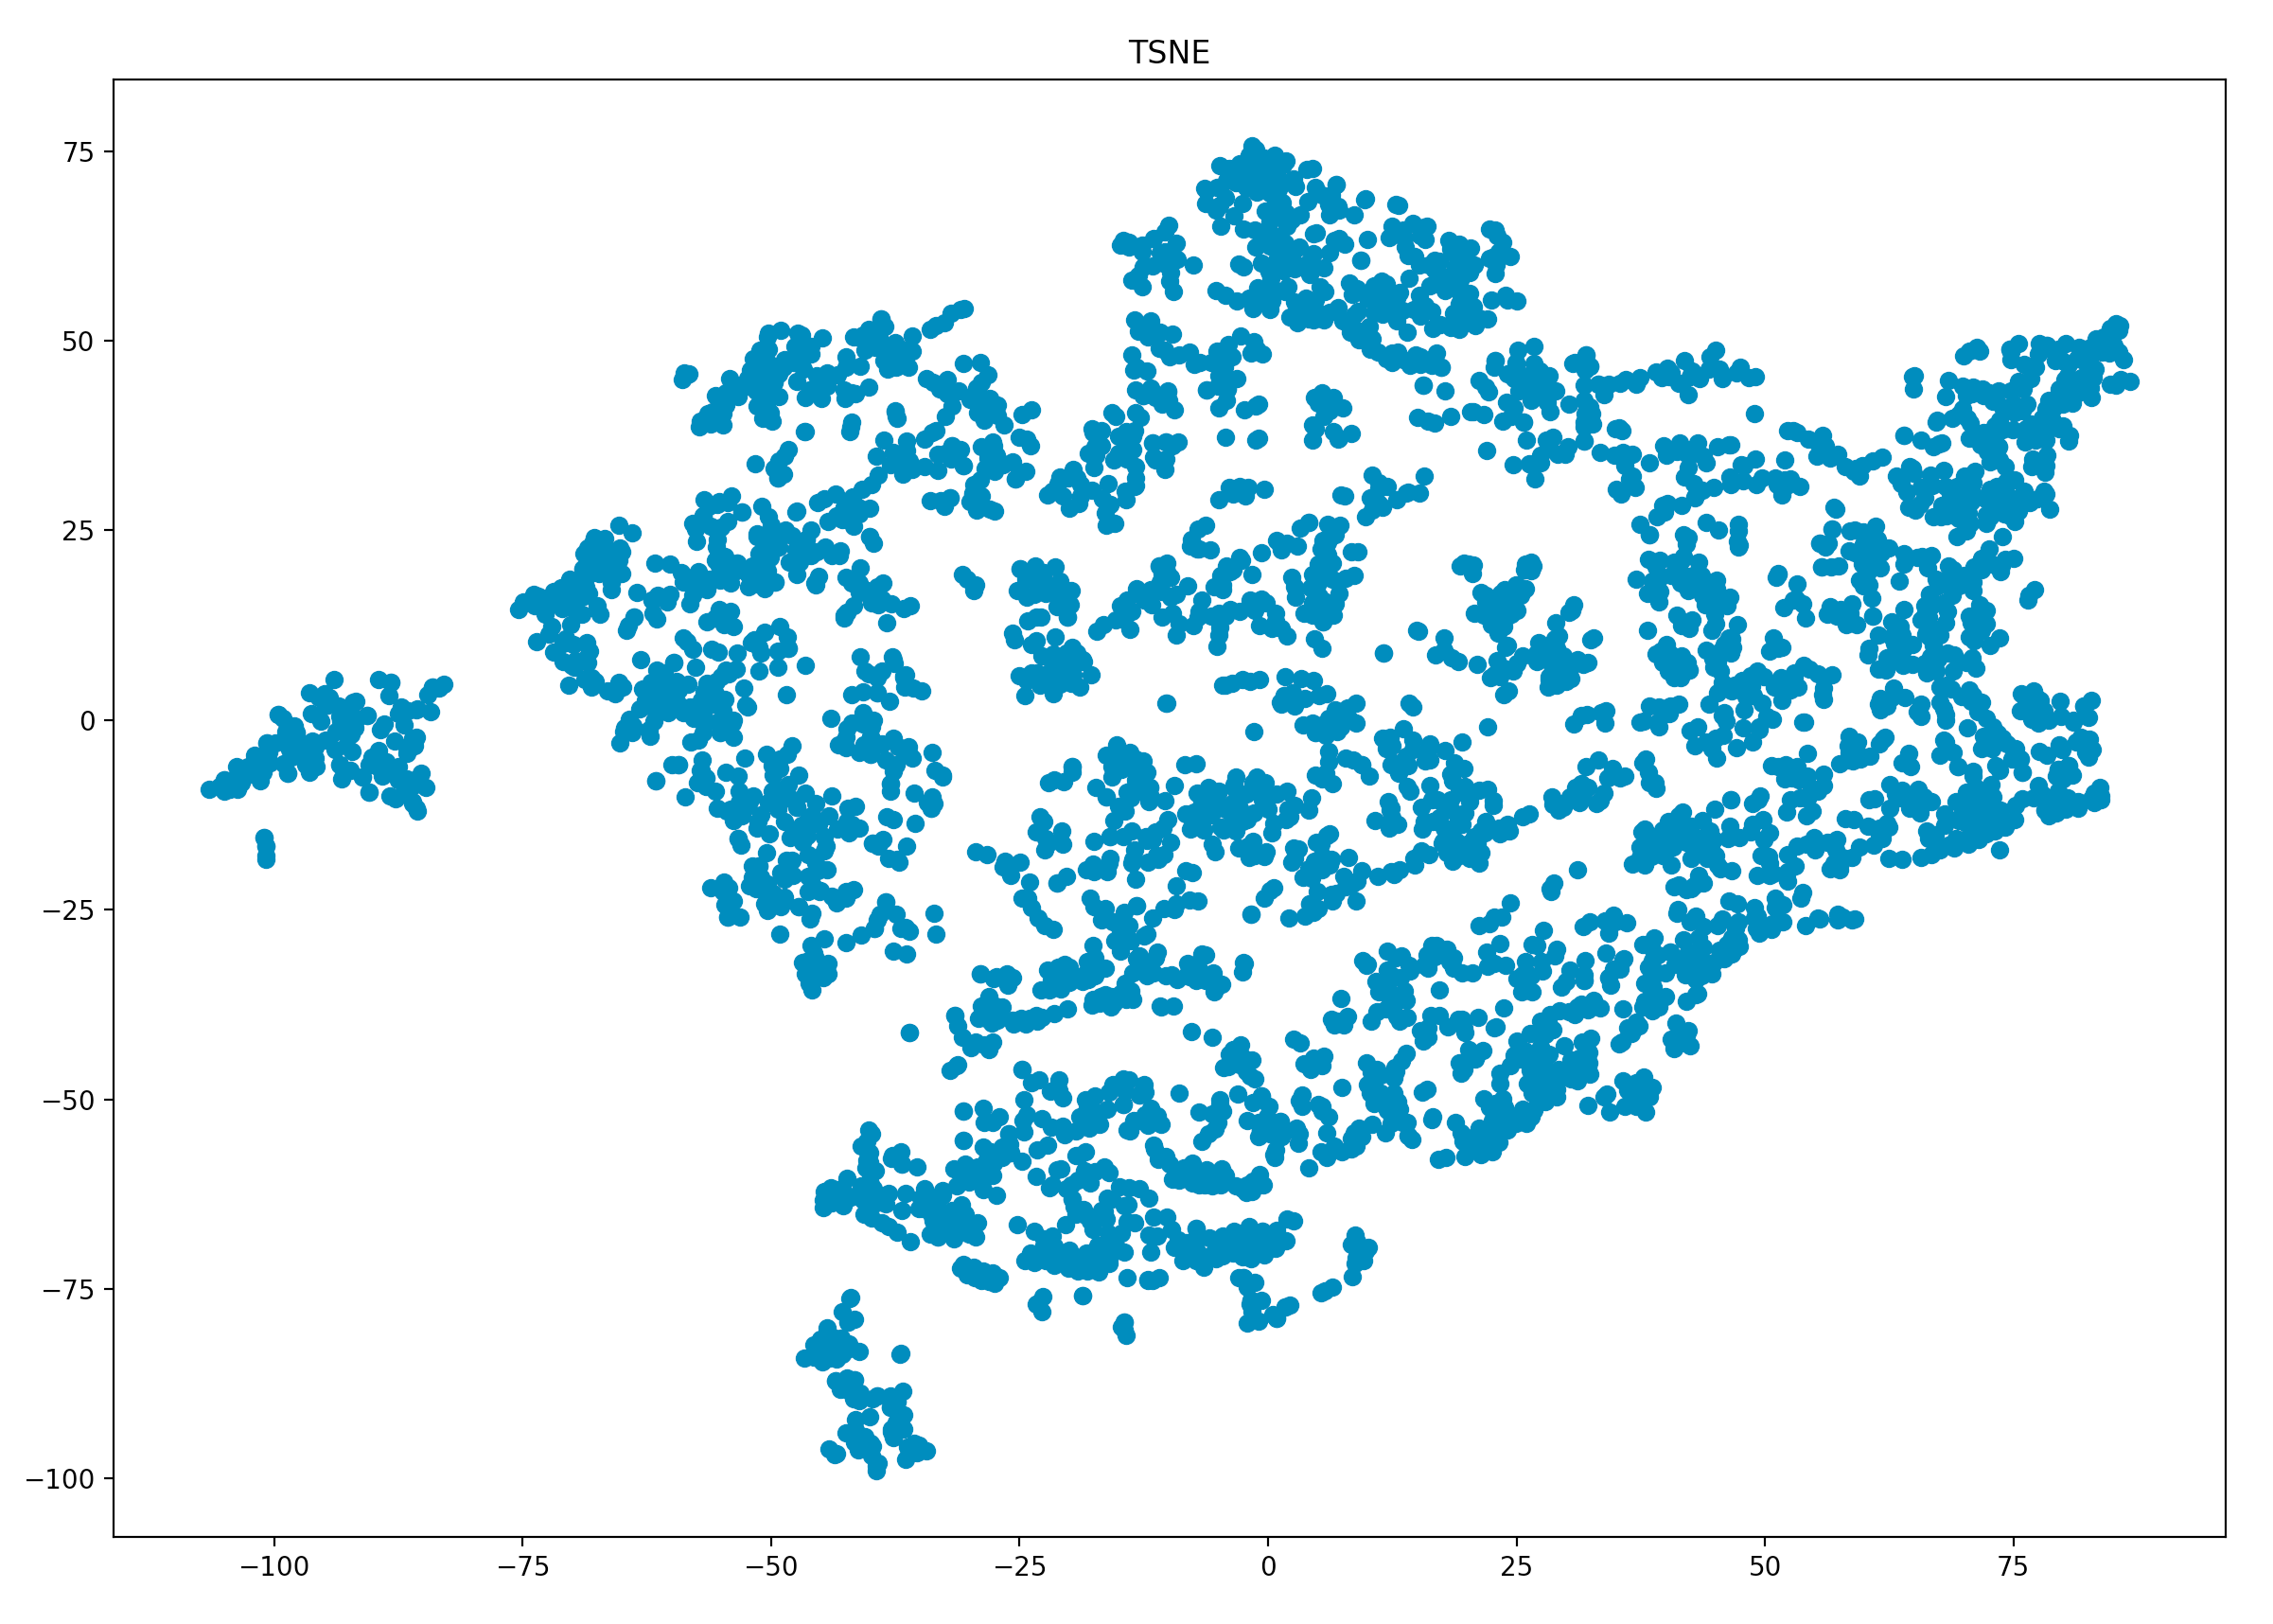
\includegraphics[width=0.9\textwidth]{./images/tsneParametersTest/learningRate/lr800-3hTSNE.png}
  \end{subfigure}%
  \begin{subfigure}{.5\textwidth}
    \centering
    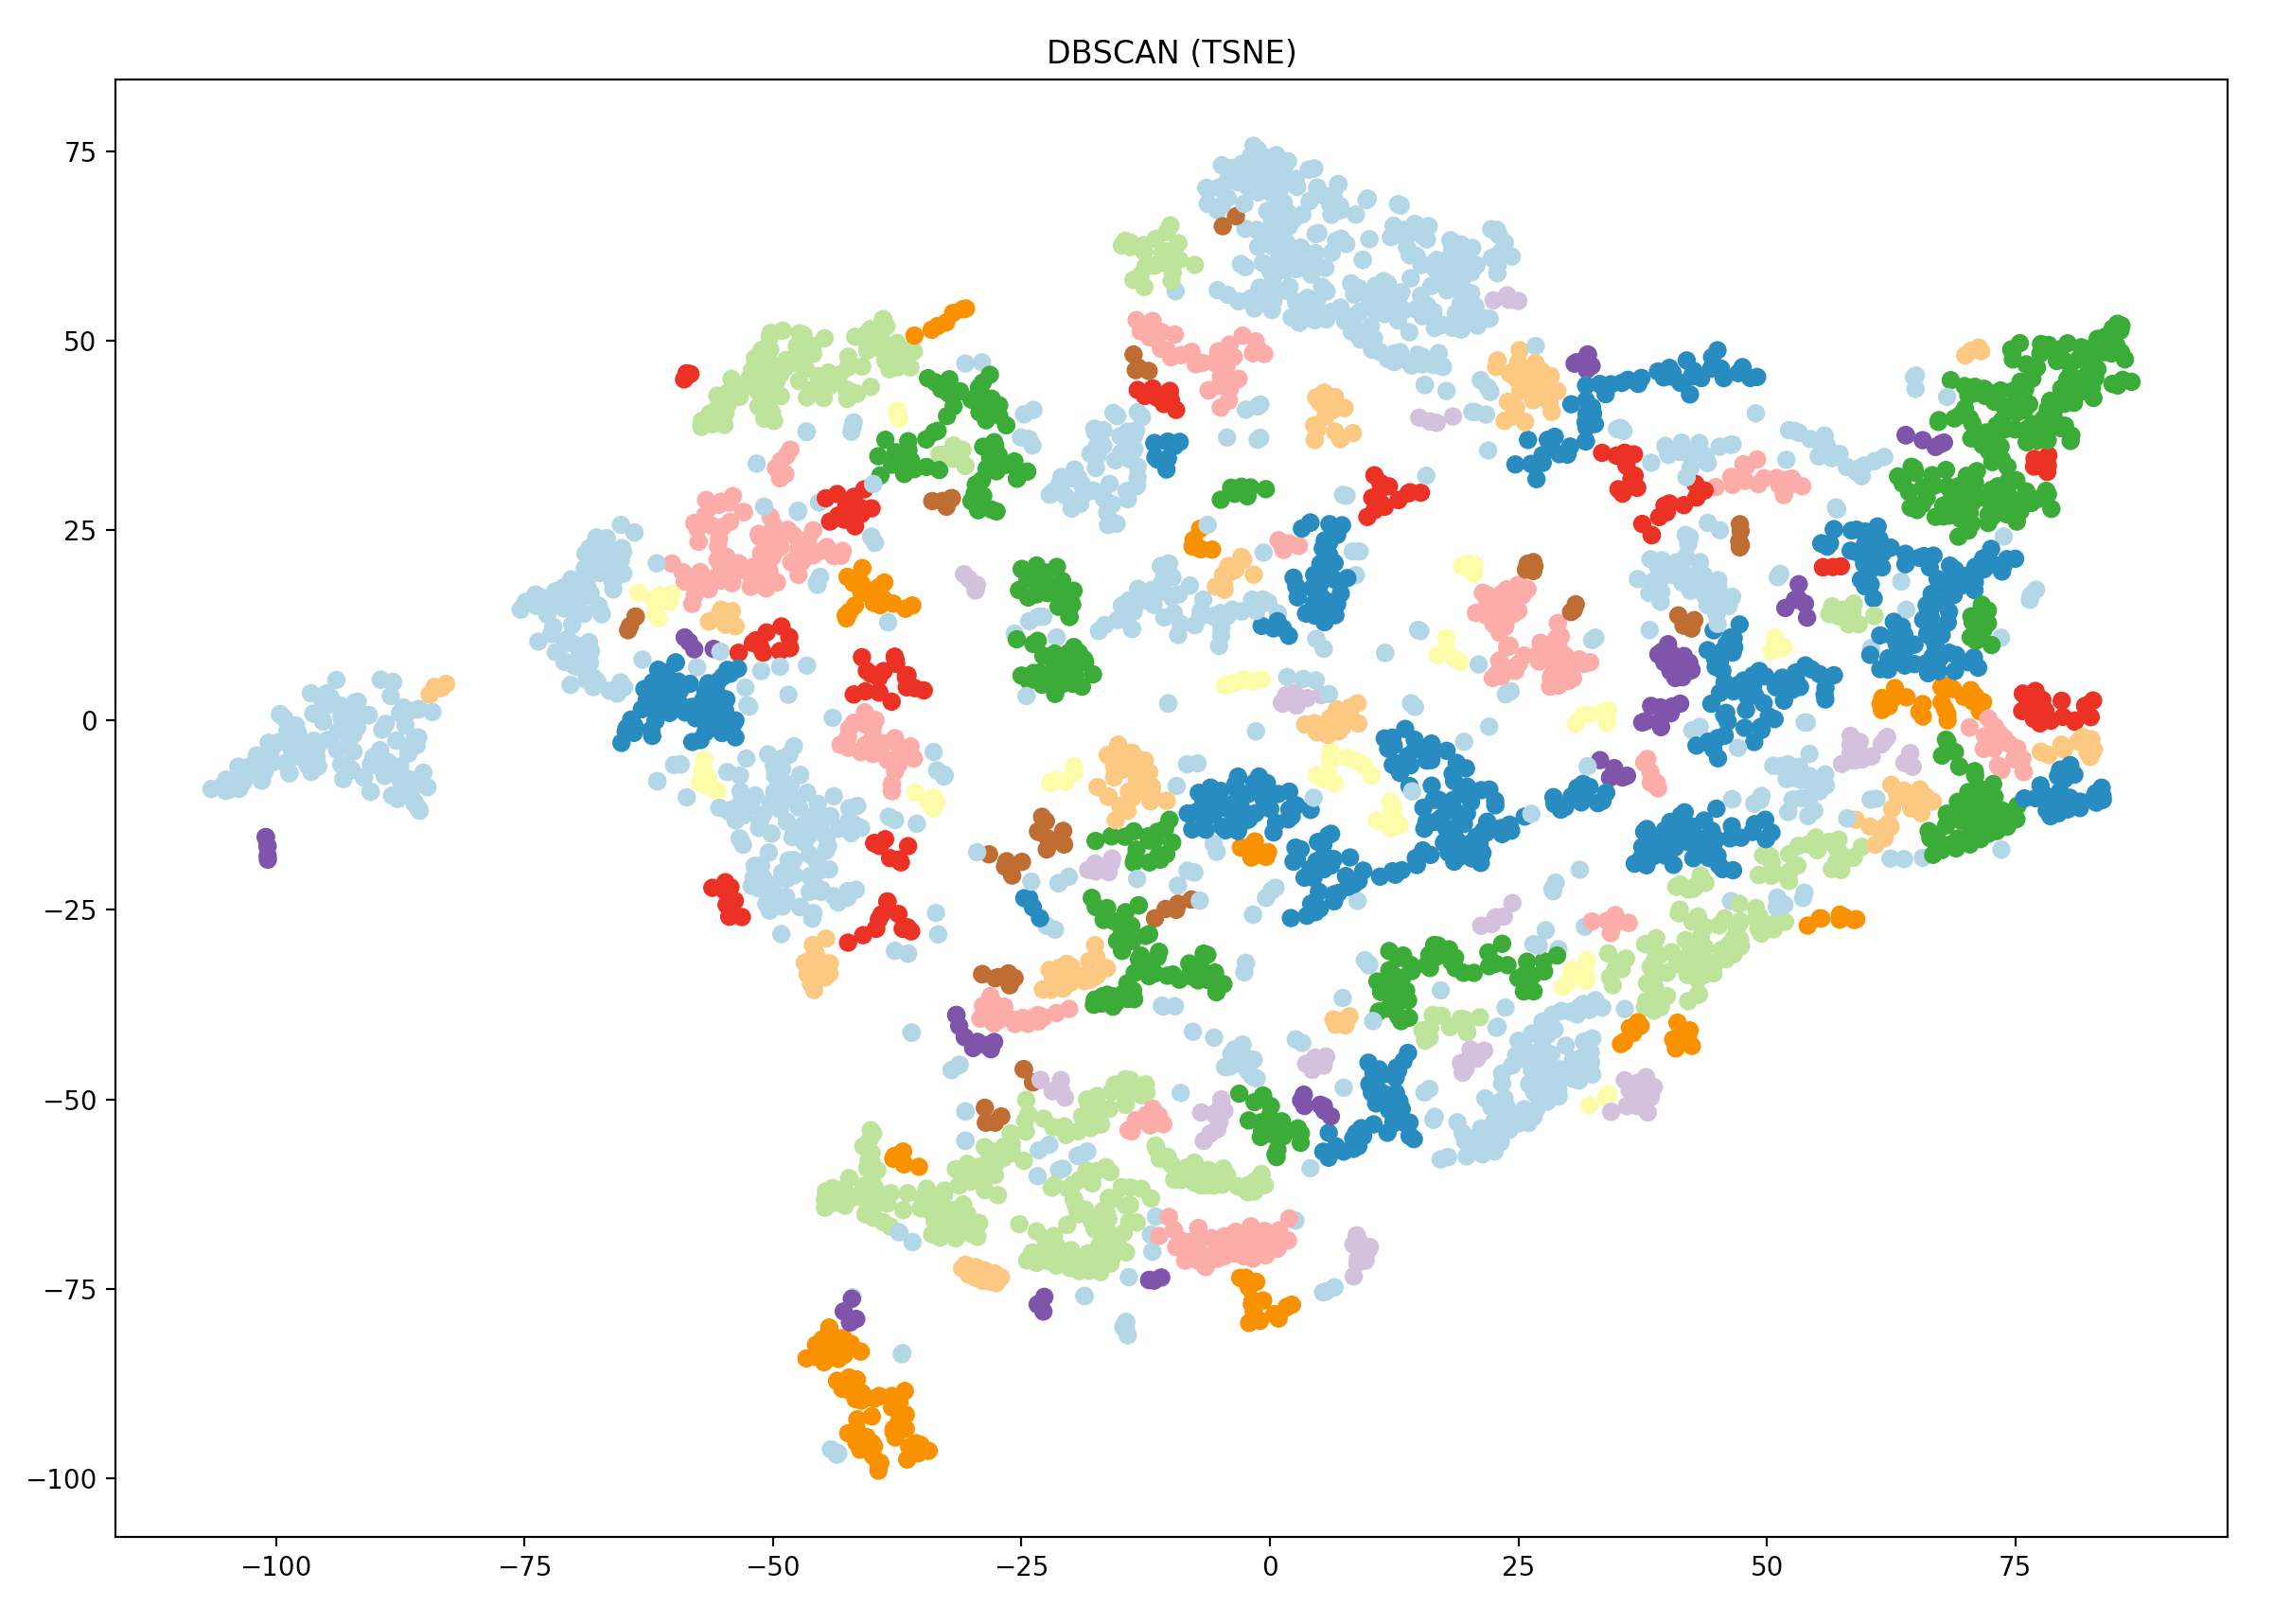
\includegraphics[width=0.9\textwidth]{./images/tsneParametersTest/learningRate/lr800-3hDBSCAN.png}
	\end{subfigure}
	\caption{\textbf{3h} data files, t-SNE calculated with the following parameters: perplexity=40, n\_iter=5000, \textbf{learning\_rate=800}}
  \label{figure:3hlr800TSNE}
\end{figure}


%------------------ LEARNING RATE 1000: ------------------
\subsubsection{Learning Rate = 1000}
% -- 1h, lr 1000 --
\begin{figure}[H]
  \centering
  \begin{subfigure}{.5\textwidth}
    \centering
    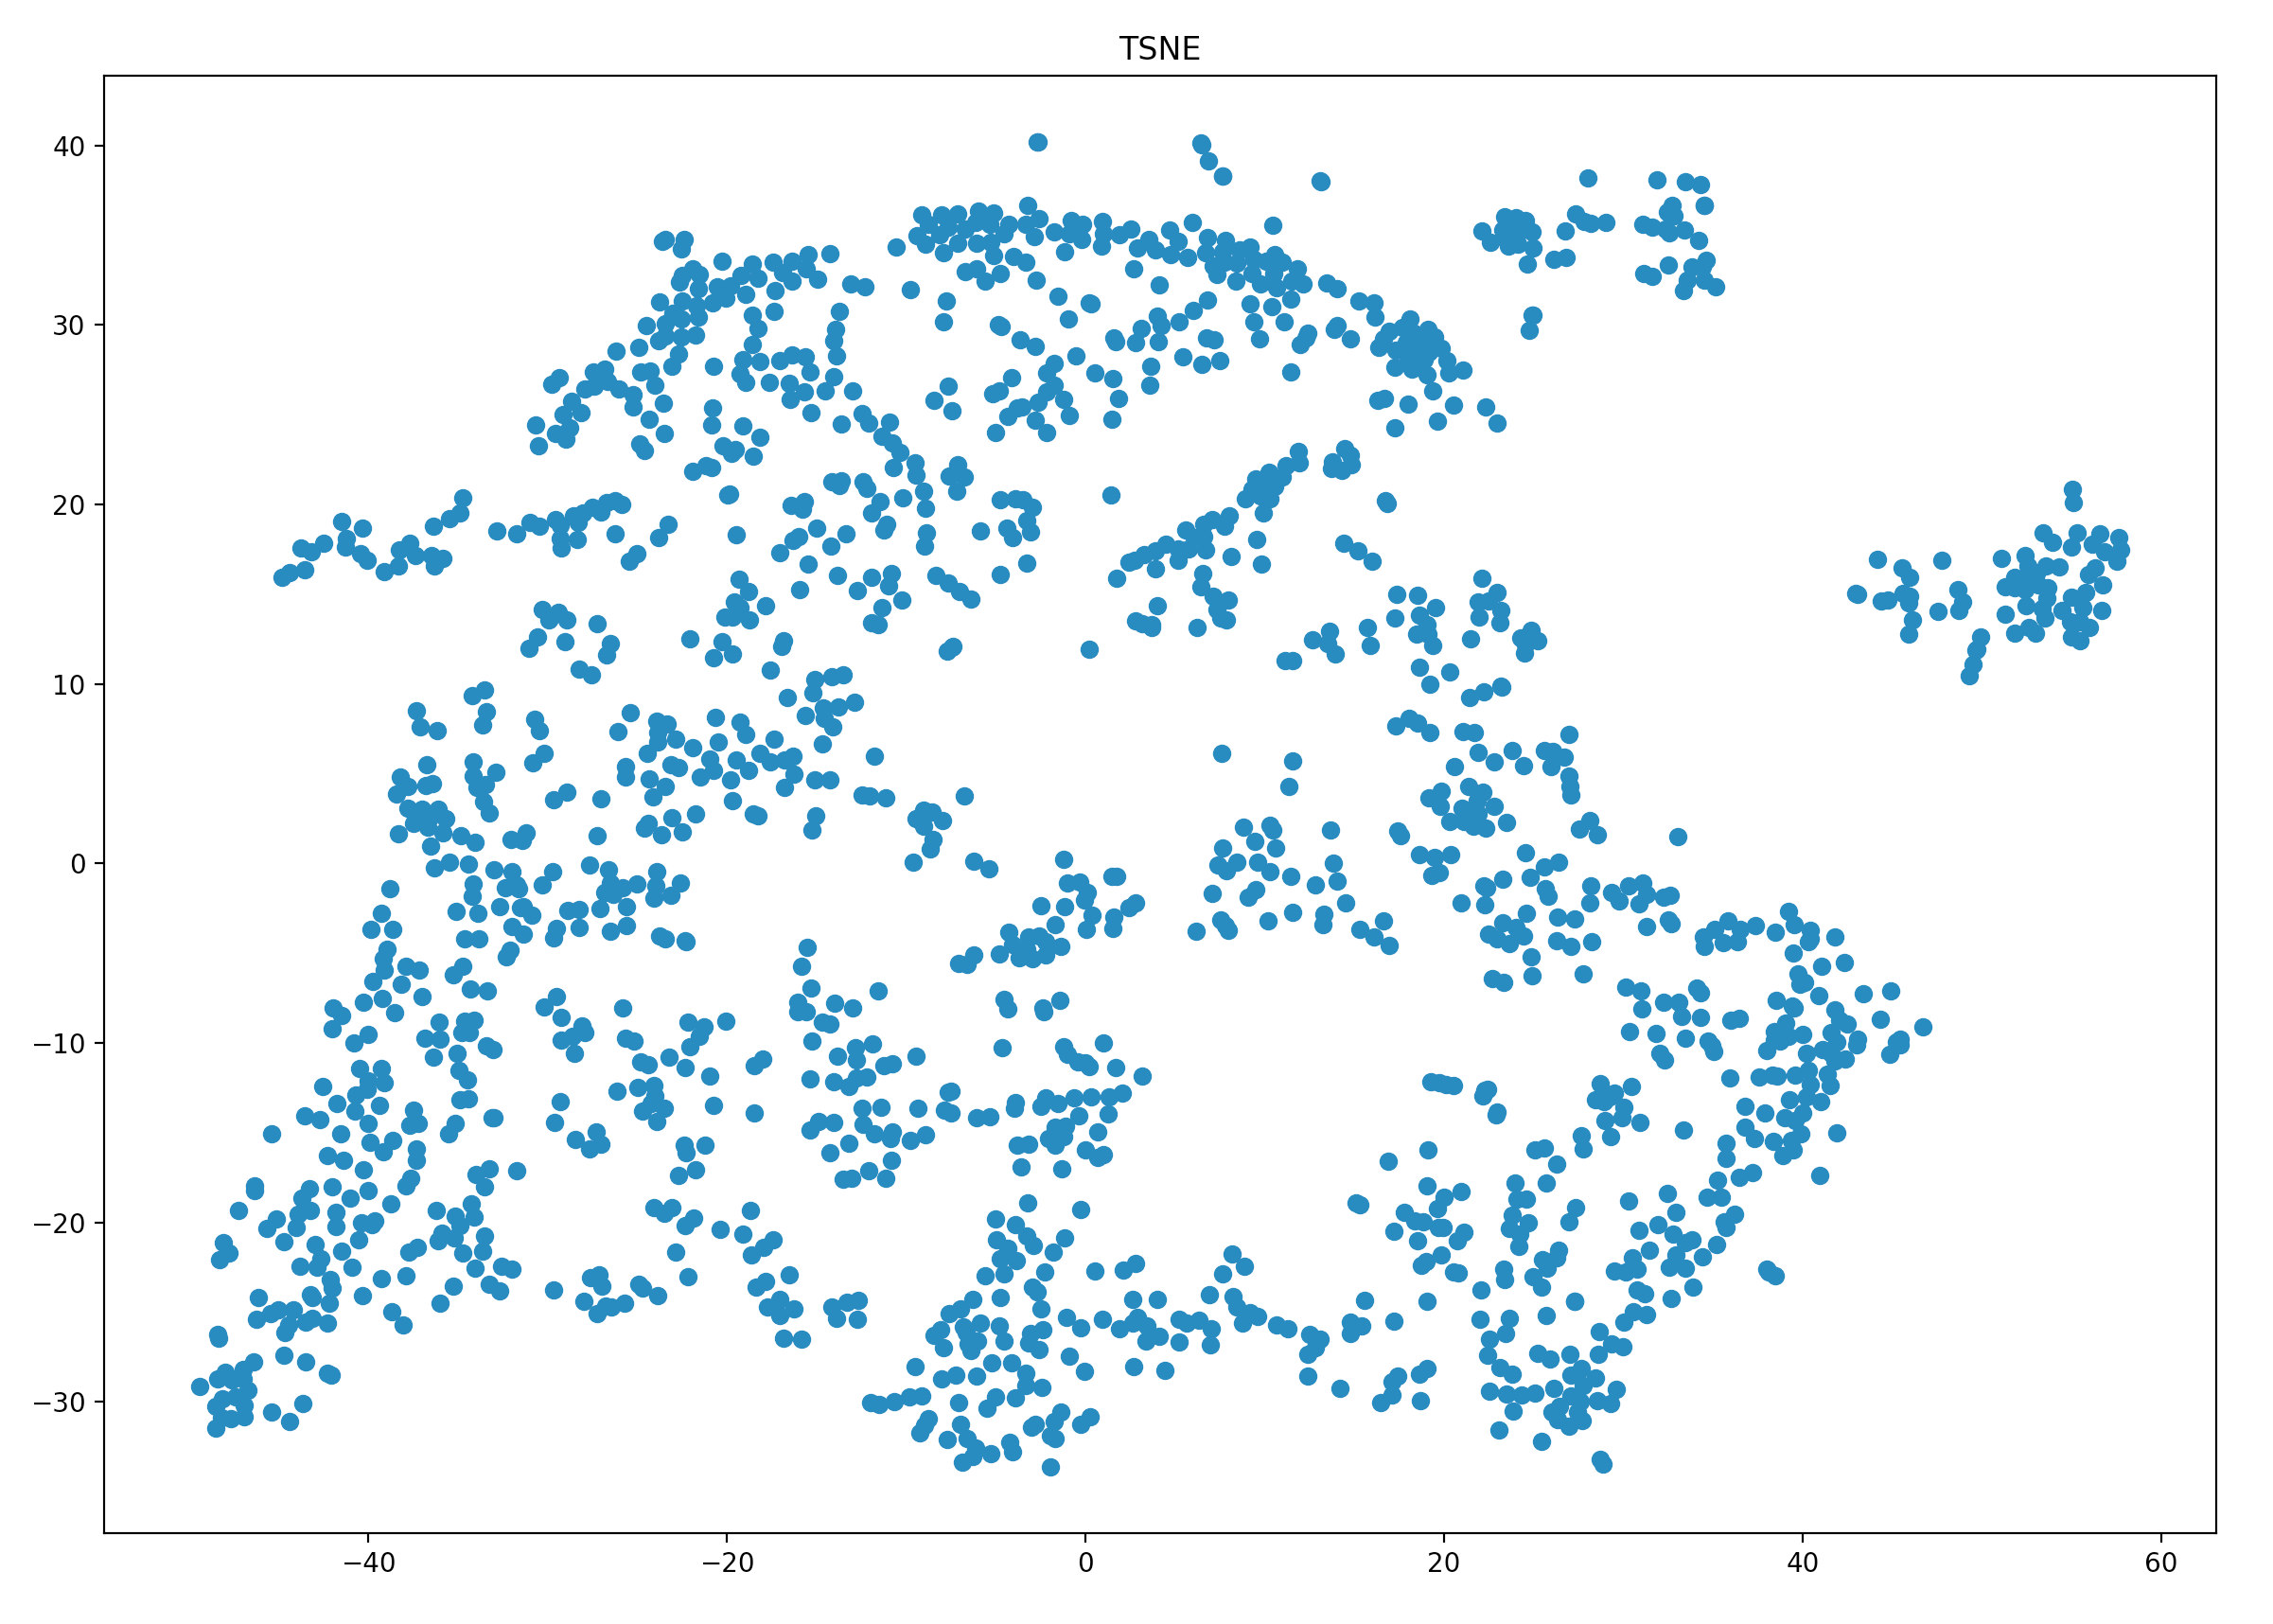
\includegraphics[width=0.9\textwidth]{./images/tsneParametersTest/learningRate/lr1000-1hTSNE.png}
  \end{subfigure}%
  \begin{subfigure}{.5\textwidth}
    \centering
    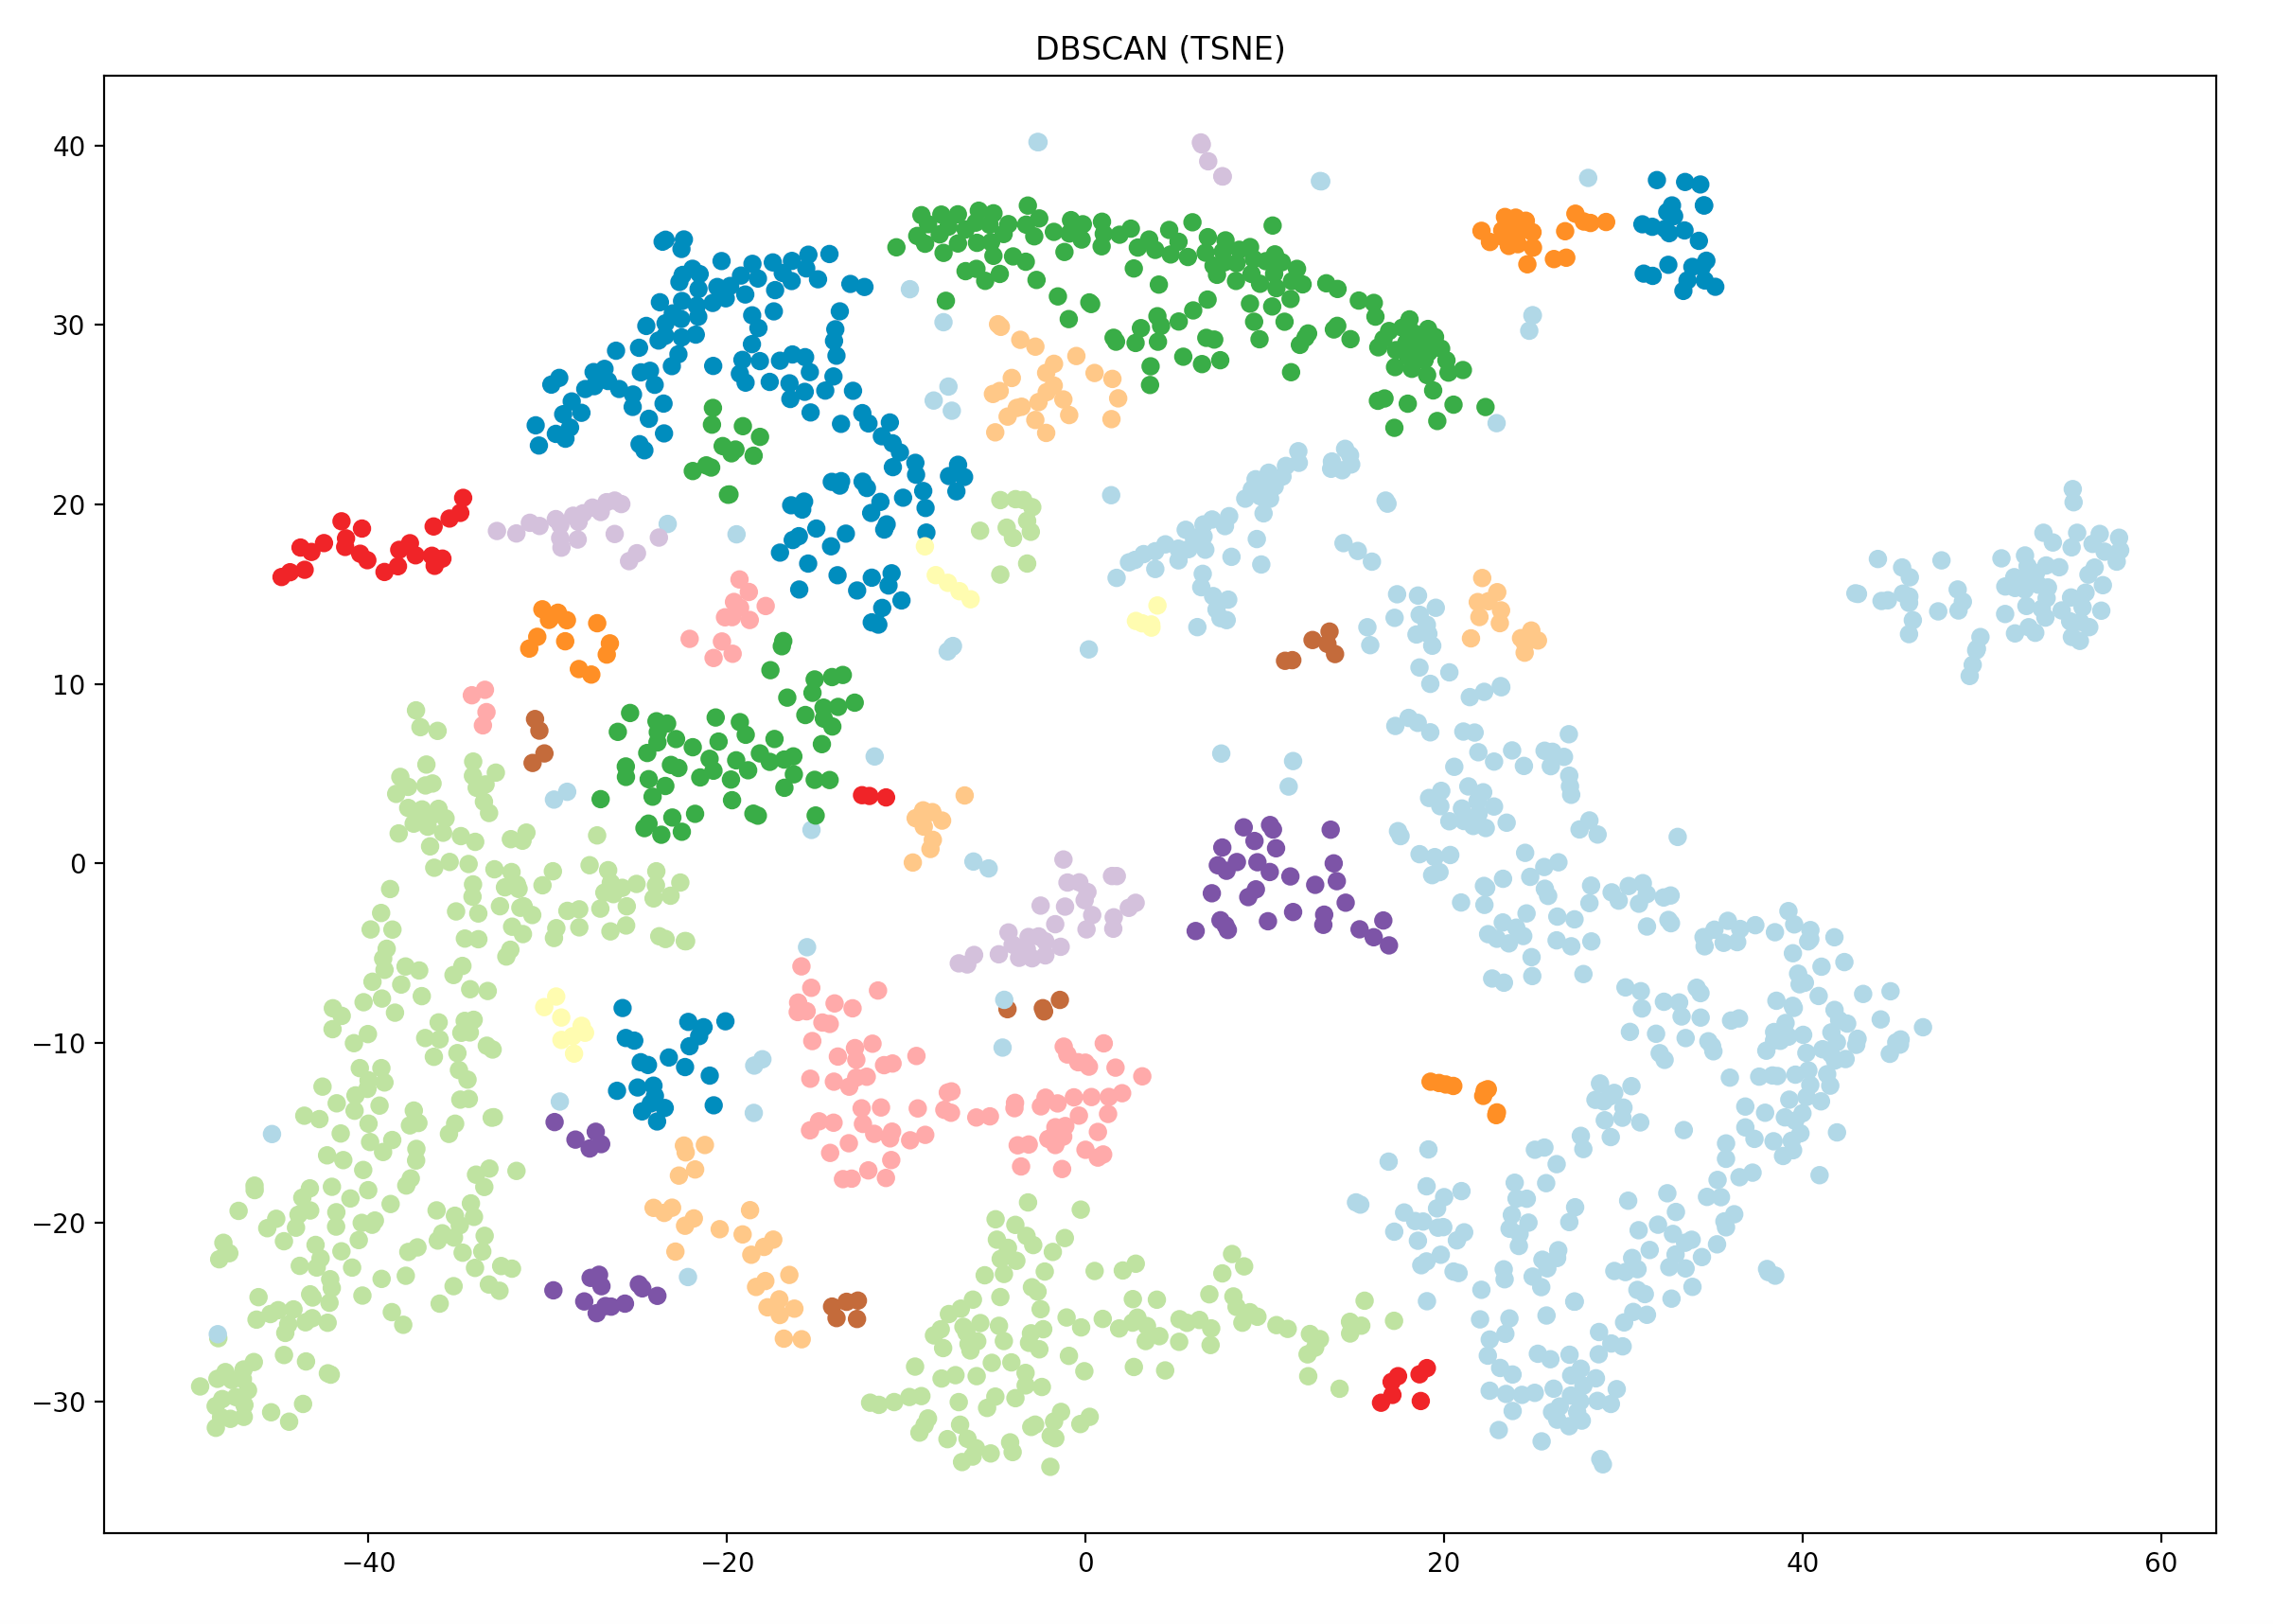
\includegraphics[width=0.9\textwidth]{./images/tsneParametersTest/learningRate/lr1000-1hDBSCAN.png}
  \end{subfigure}
	\caption{\textbf{1h} data files, t-SNE calculated with the following parameters: perplexity=40, n\_iter=5000, \textbf{learning\_rate=1000}}
	\label{figure:1hlr1000TSNE}
\end{figure}

% -- 3h, lr 1000 --
\begin{figure}[H]
	\centering
	
  \centering
	\begin{subfigure}{.5\textwidth}
    \centering
    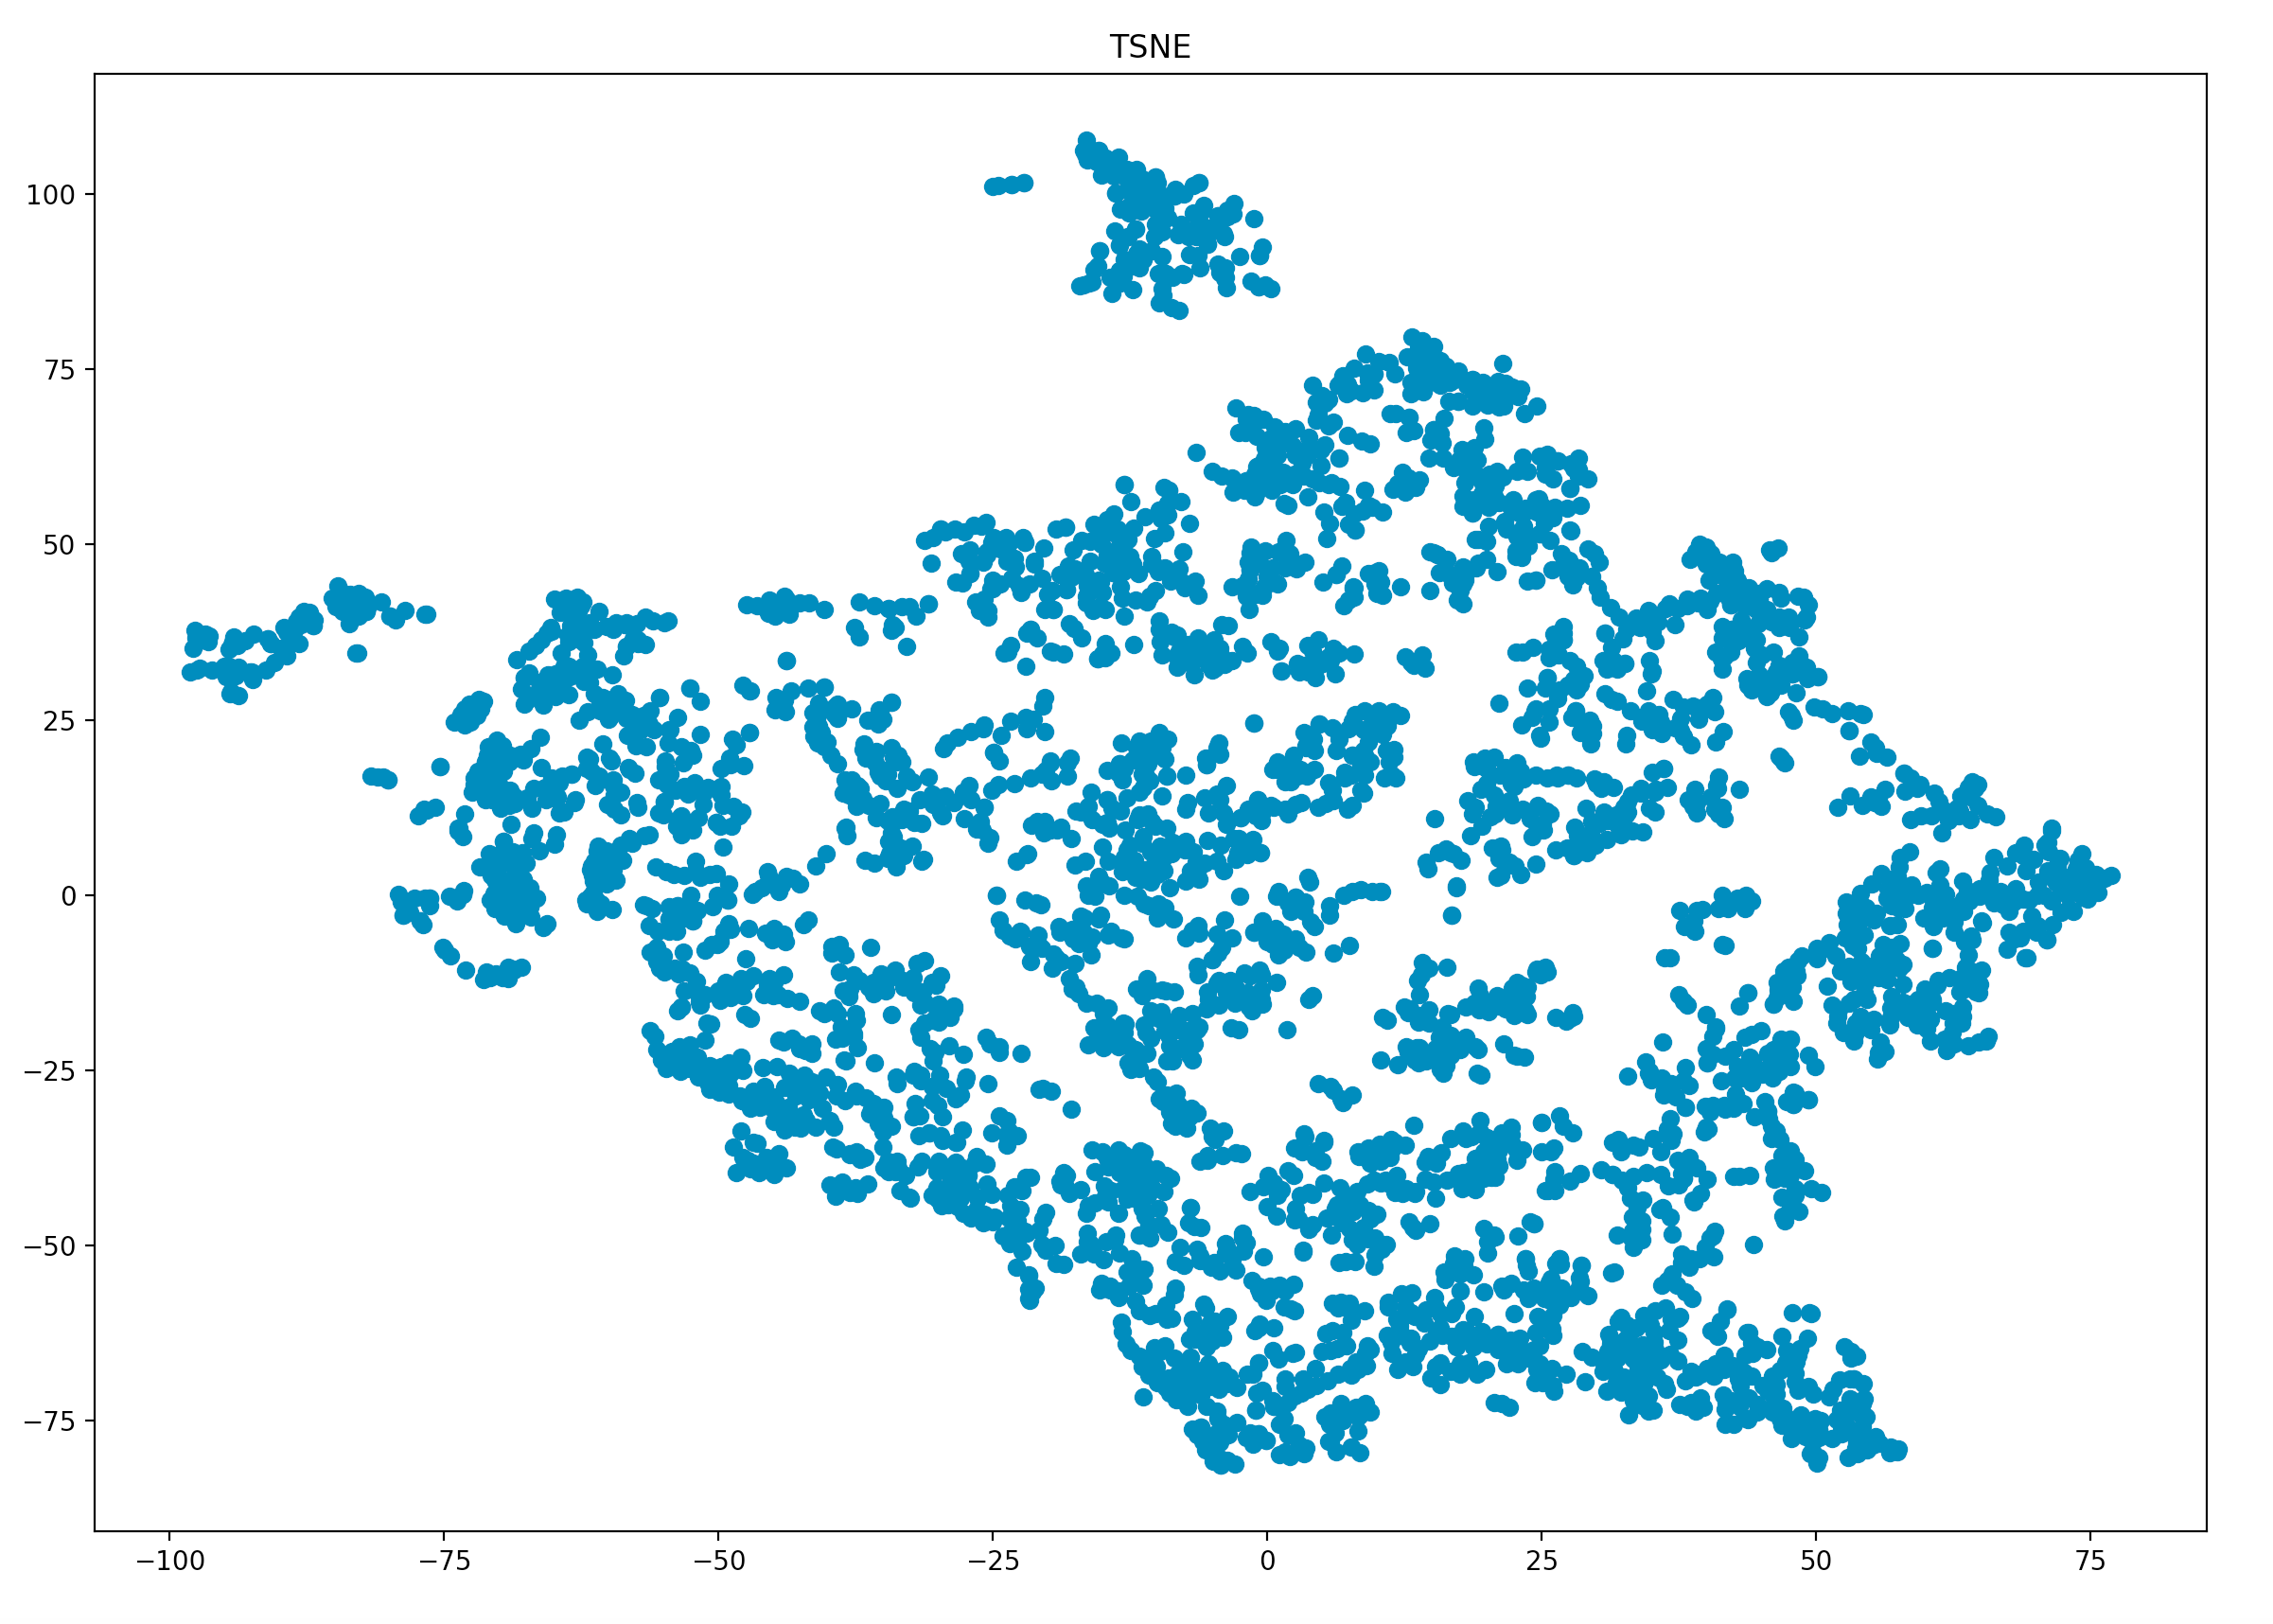
\includegraphics[width=0.9\textwidth]{./images/tsneParametersTest/learningRate/lr1000-3hTSNE.png}
  \end{subfigure}%
  \begin{subfigure}{.5\textwidth}
    \centering
    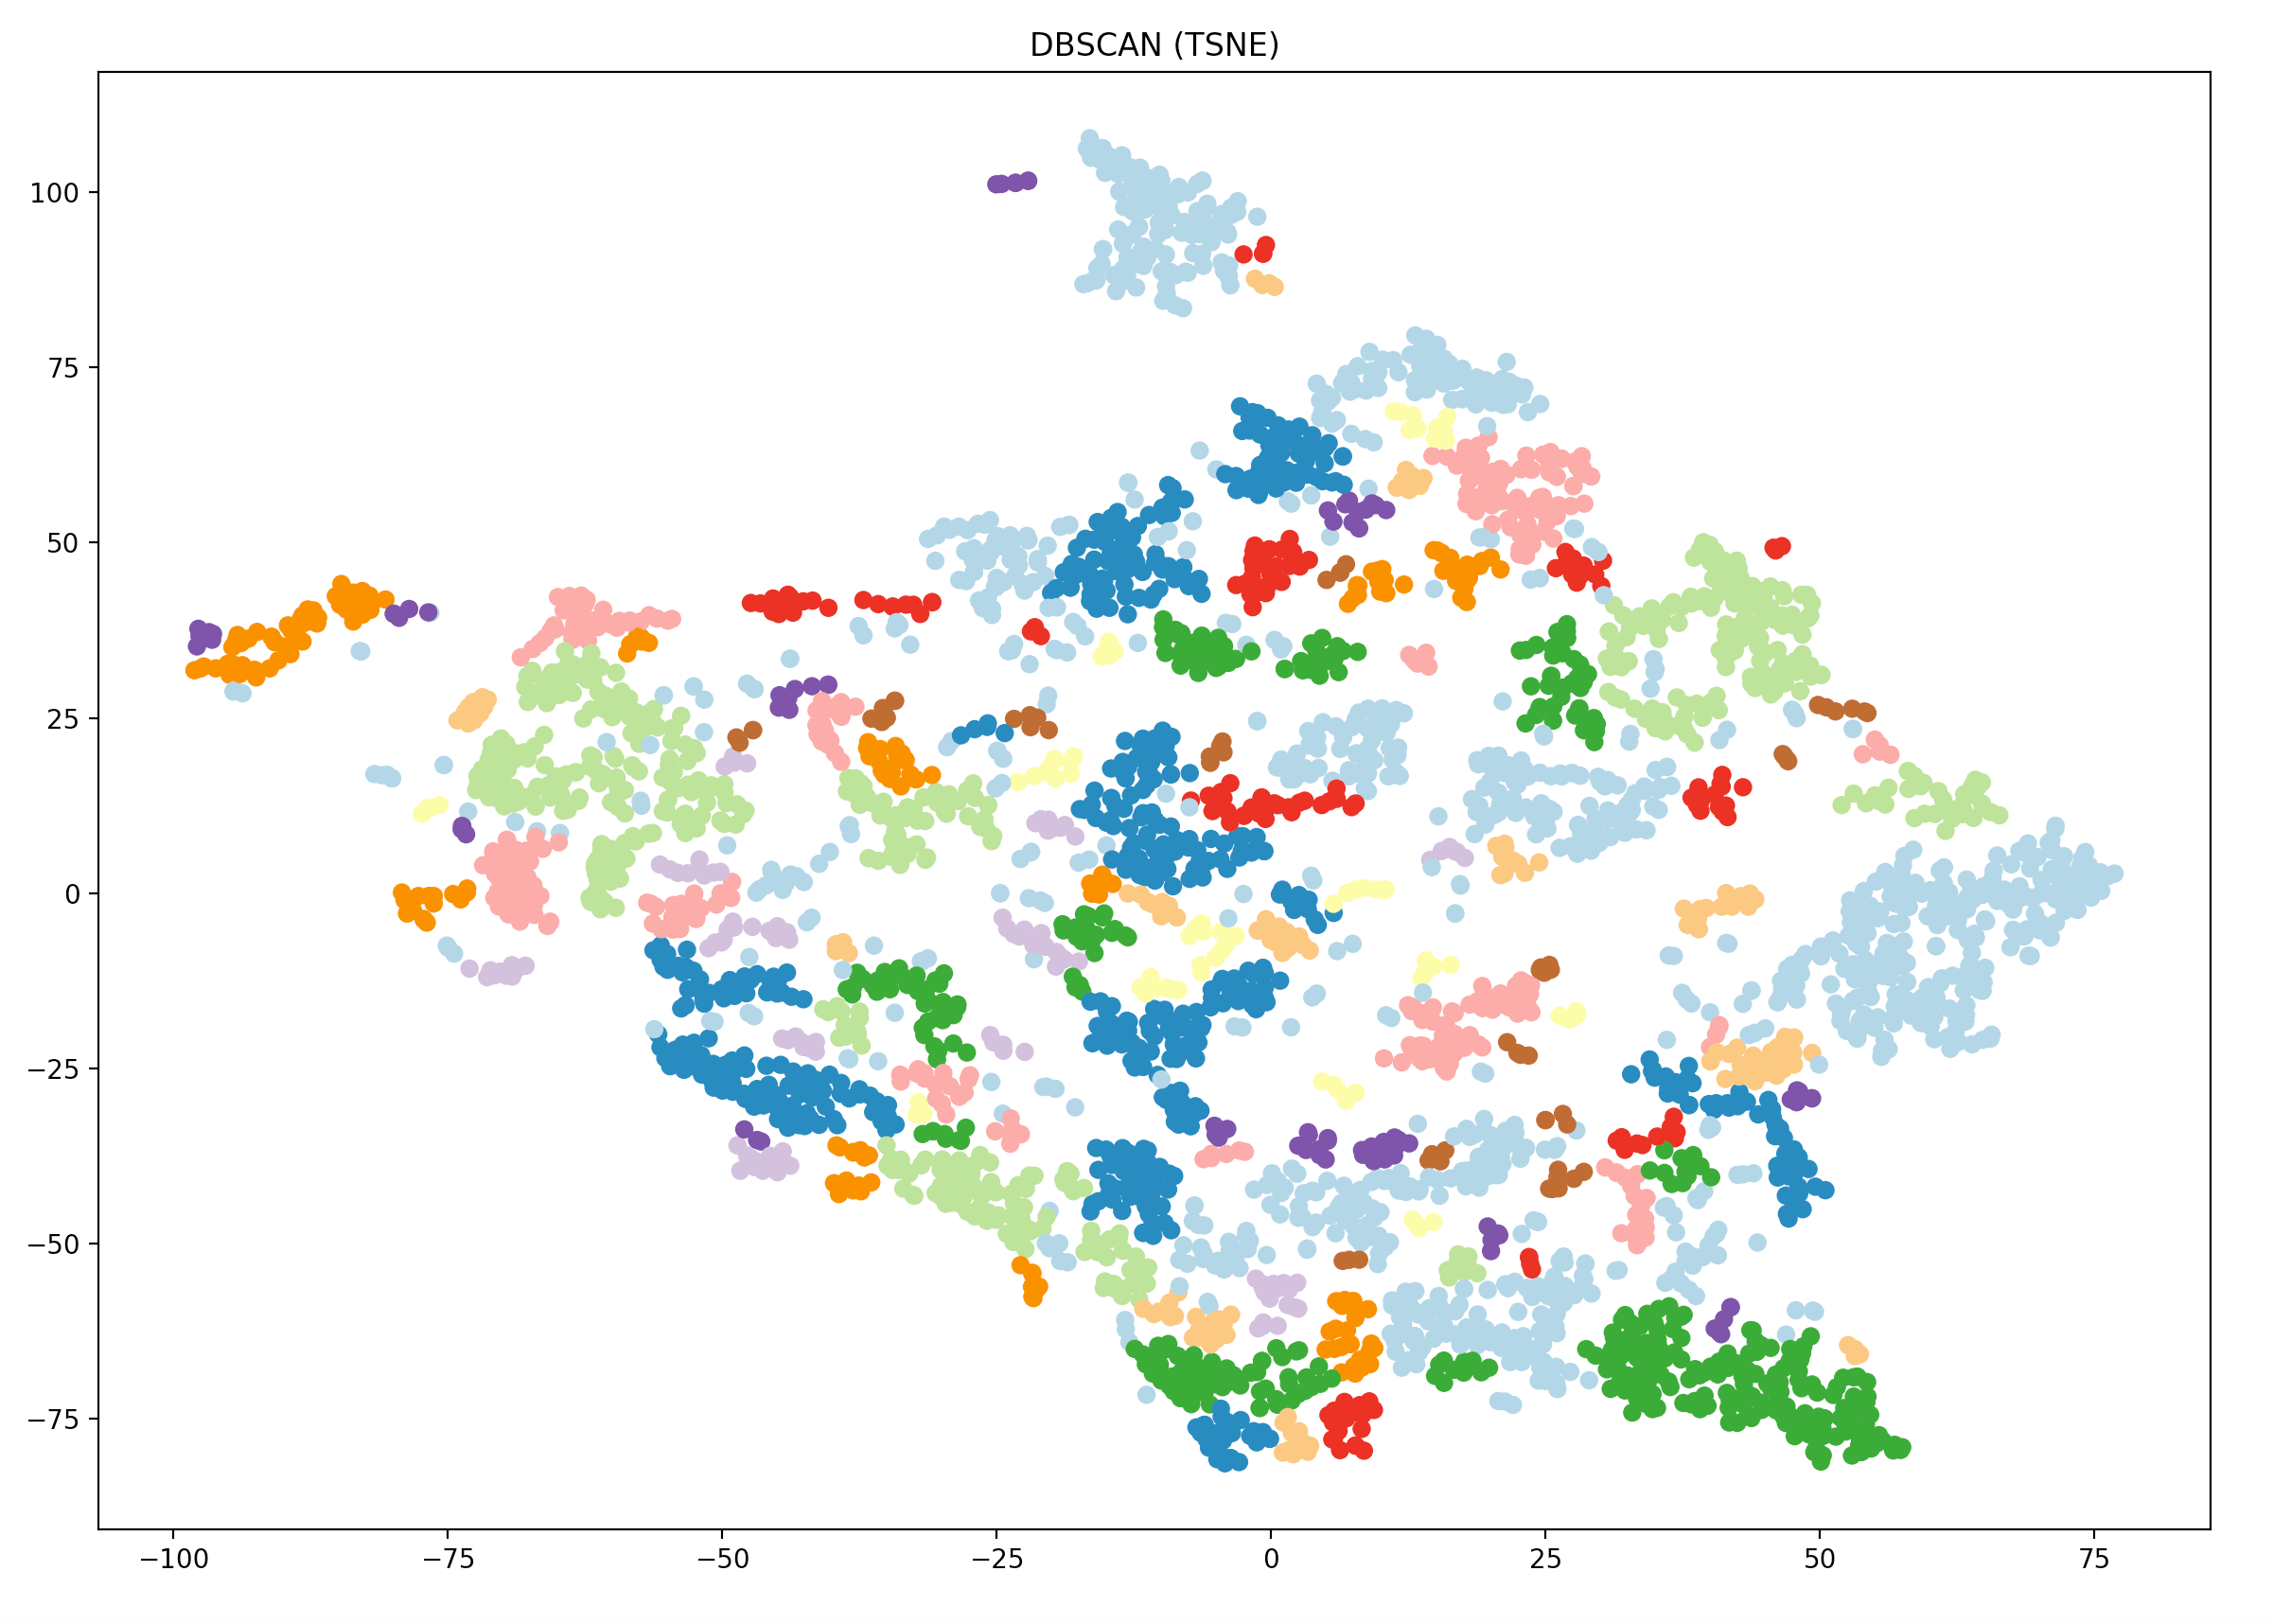
\includegraphics[width=0.9\textwidth]{./images/tsneParametersTest/learningRate/lr1000-3hDBSCAN.png}
	\end{subfigure}
	\caption{\textbf{3h} data files, t-SNE calculated with the following parameters: perplexity=40, n\_iter=5000, \textbf{learning\_rate=1000}}
  \label{figure:3hlr1000TSNE}
\end{figure}



\subsubsection{Learning Rate Detailed Comparison Results }
\label{appendix:comparelearningRateDetailed}

\begin{figure}
  \centering
  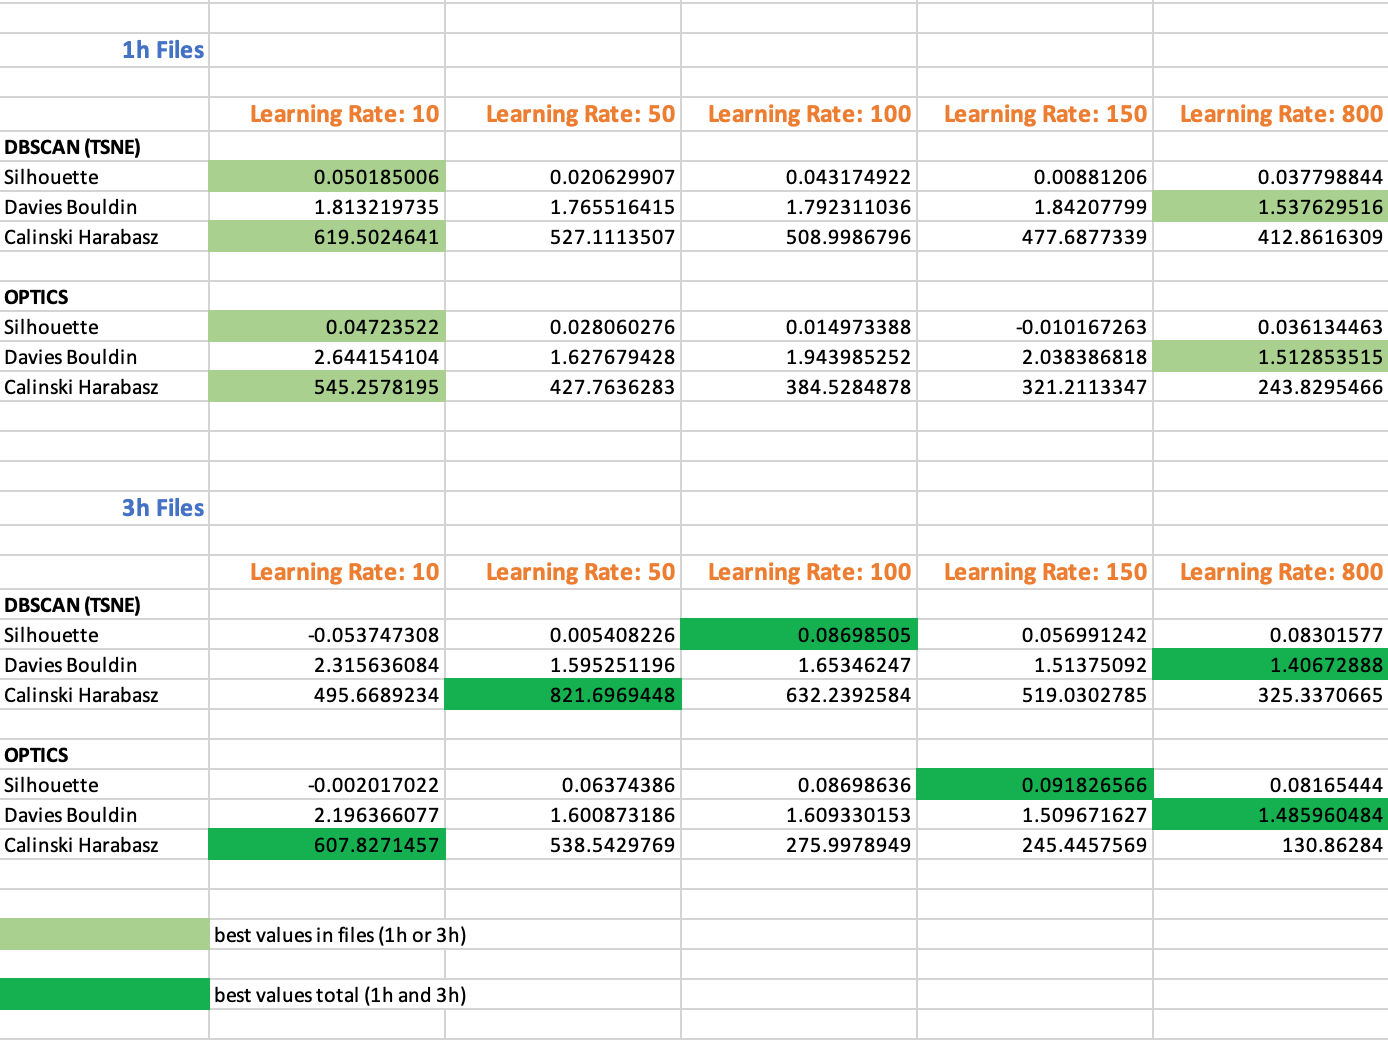
\includegraphics[width=0.8\textwidth]{./images/tsneParametersTest/learningRate/learningRateEvaluationScoresDetailed.png}
  \caption{Comparison of Silhouette Coefficient, Davies-Bouldin Index, and Caliński-Harabasz Index for different t-SNE \textbf{learning rate} values. Smaller learning rate value steps were taken (i.e. 50, except for the first step which is 40 and the last step to 800) between each test. The lighter green highlighted values indicate the best values of that file aggregation (1h or 3h files). The dark green highlighted values illustrate the overall best values over all files (1h and 3h files).}
  \label{figure:learningRateEvaluationScoresDetailed}
\end{figure}

\begin{figure}
  \centering
  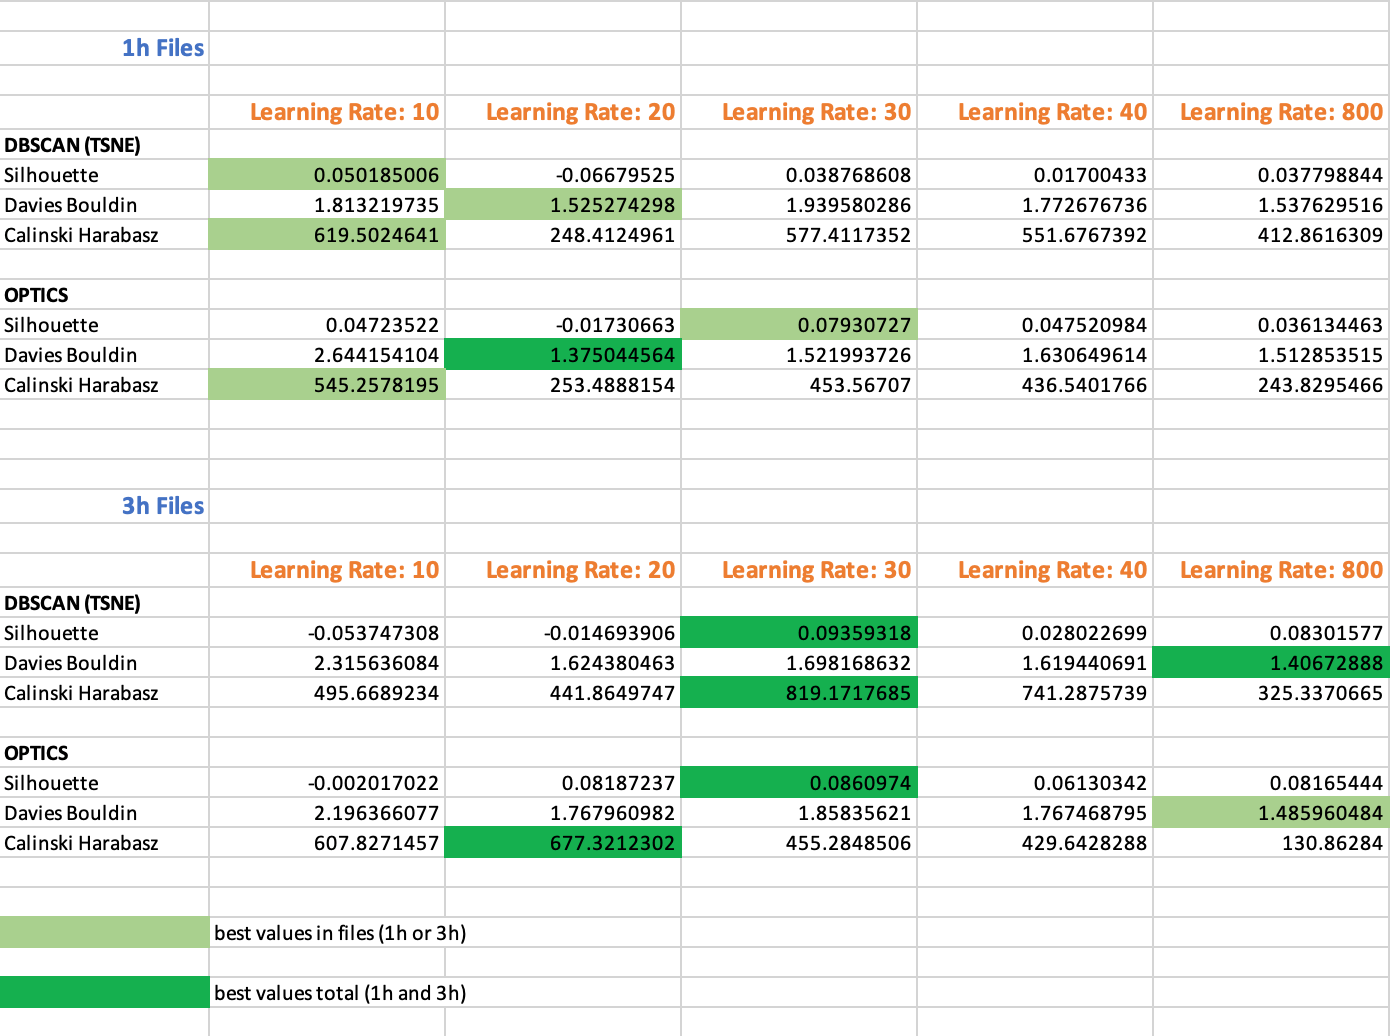
\includegraphics[width=0.8\textwidth]{./images/tsneParametersTest/learningRate/learningRateEvaluationScoresDetailed2.png}
  \caption{Comparison of Silhouette Coefficient, Davies-Bouldin Index, and Caliński-Harabasz Index for different t-SNE \textbf{learning rate} values. Smaller learning rate value steps were taken (i.e. 10, except for the last step to 800) between each test. The lighter green highlighted values indicate the best values of that file aggregation (1h or 3h files). The dark green highlighted values illustrate the overall best values over all files (1h and 3h files).}
  \label{figure:learningRateEvaluationScoresDetailed2}
\end{figure}

%.................................COMPARISON AVERAGES..................................
\subsubsection{Learning Rate Comparison Results (Average of two different t-SNE runs)}
\label{appendix:compareAverageLearningRate}


\begin{figure}[H]
  \centering
  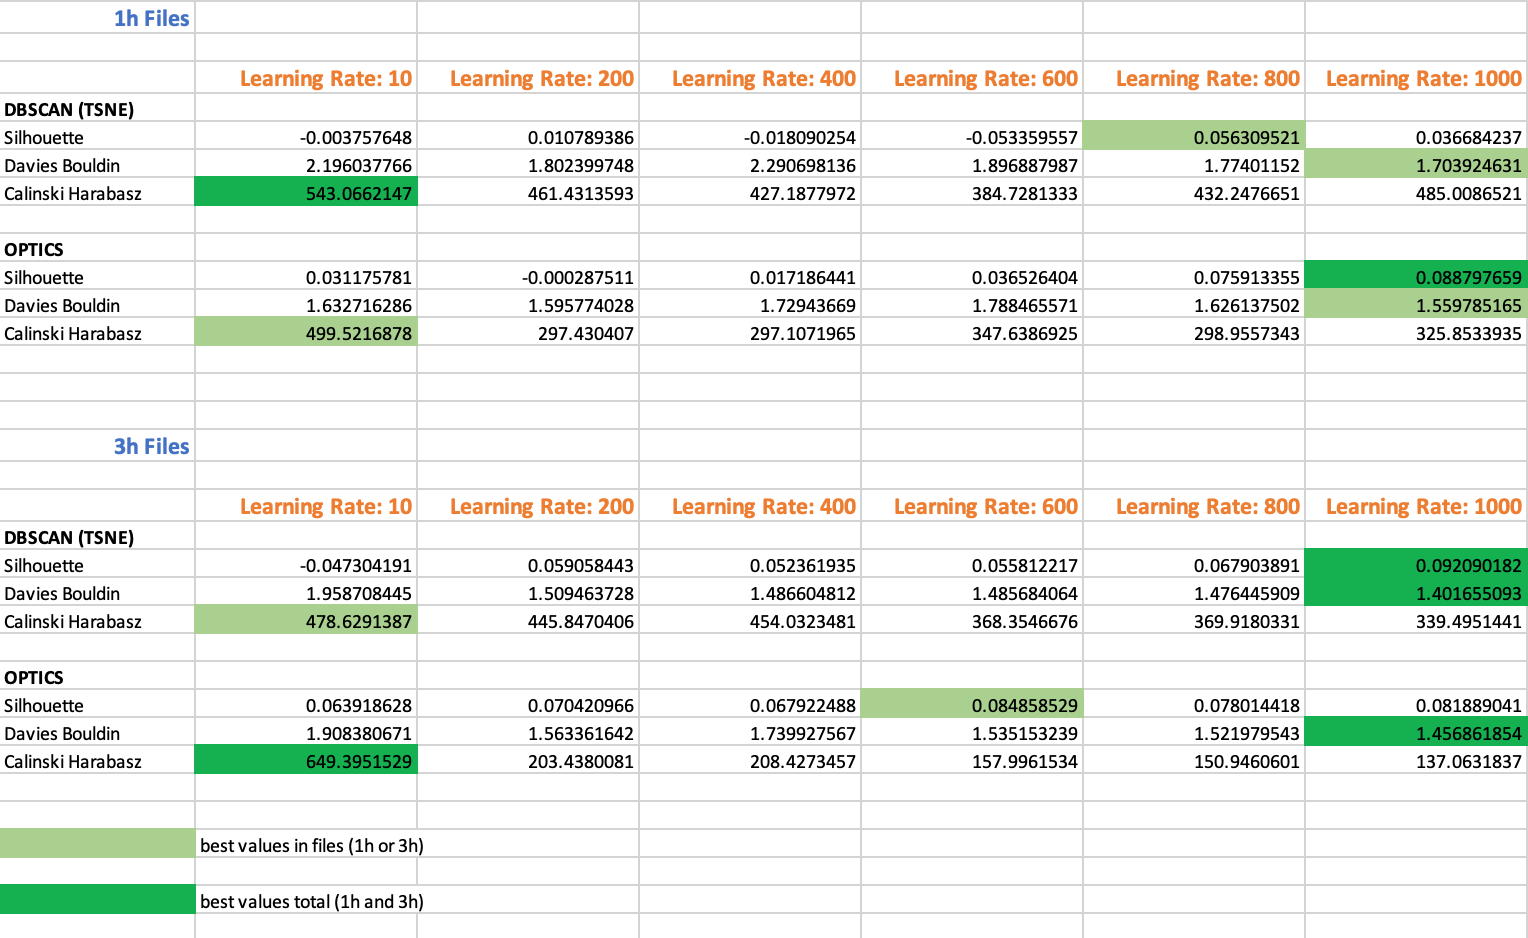
\includegraphics[width=0.8\textwidth]{./images/tsneParametersTest/learningRate/learningRateEvaluationScoresAverage.png}
  \caption{Comparison of Silhouette Coefficient, Davies-Bouldin Index, and Caliński-Harabasz Index for different t-SNE \textbf{learning rate} values, in steps of 200 (except the first step of 190). The lighter green highlighted values indicate the best values of that file aggregation (1h or 3h files). The dark green highlighted values illustrate the overall best values over all files (1h and 3h files).}
  \label{figure:learningRateEvaluationScoresAverage}
\end{figure}

\begin{figure}[H]
  \centering
  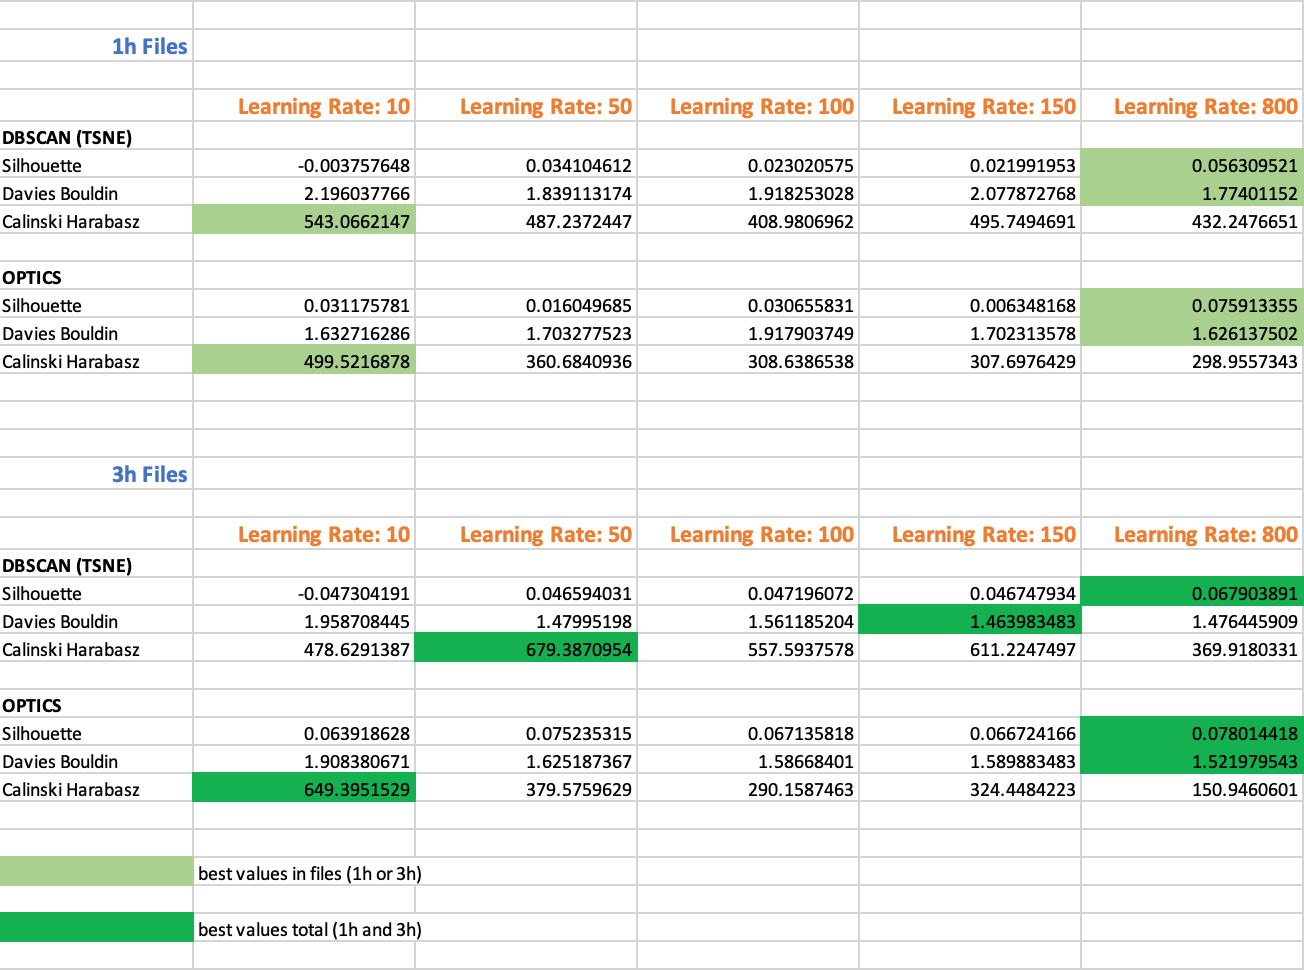
\includegraphics[width=0.8\textwidth]{./images/tsneParametersTest/learningRate/learningRateEvaluationScoresAverageDetailed.png}
  \caption{Comparison of Silhouette Coefficient, Davies-Bouldin Index, and Caliński-Harabasz Index for different t-SNE \textbf{learning rate} values. Smaller learning rate value steps were taken (i.e. 50, except for the first step which is 40 and the last step to 800) between each test. The lighter green highlighted values indicate the best values of that file aggregation (1h or 3h files). The dark green highlighted values illustrate the overall best values over all files (1h and 3h files).}
  \label{figure:learningRateEvaluationScoresAverageDetailed}
\end{figure}

\begin{figure}[H]
  \centering
  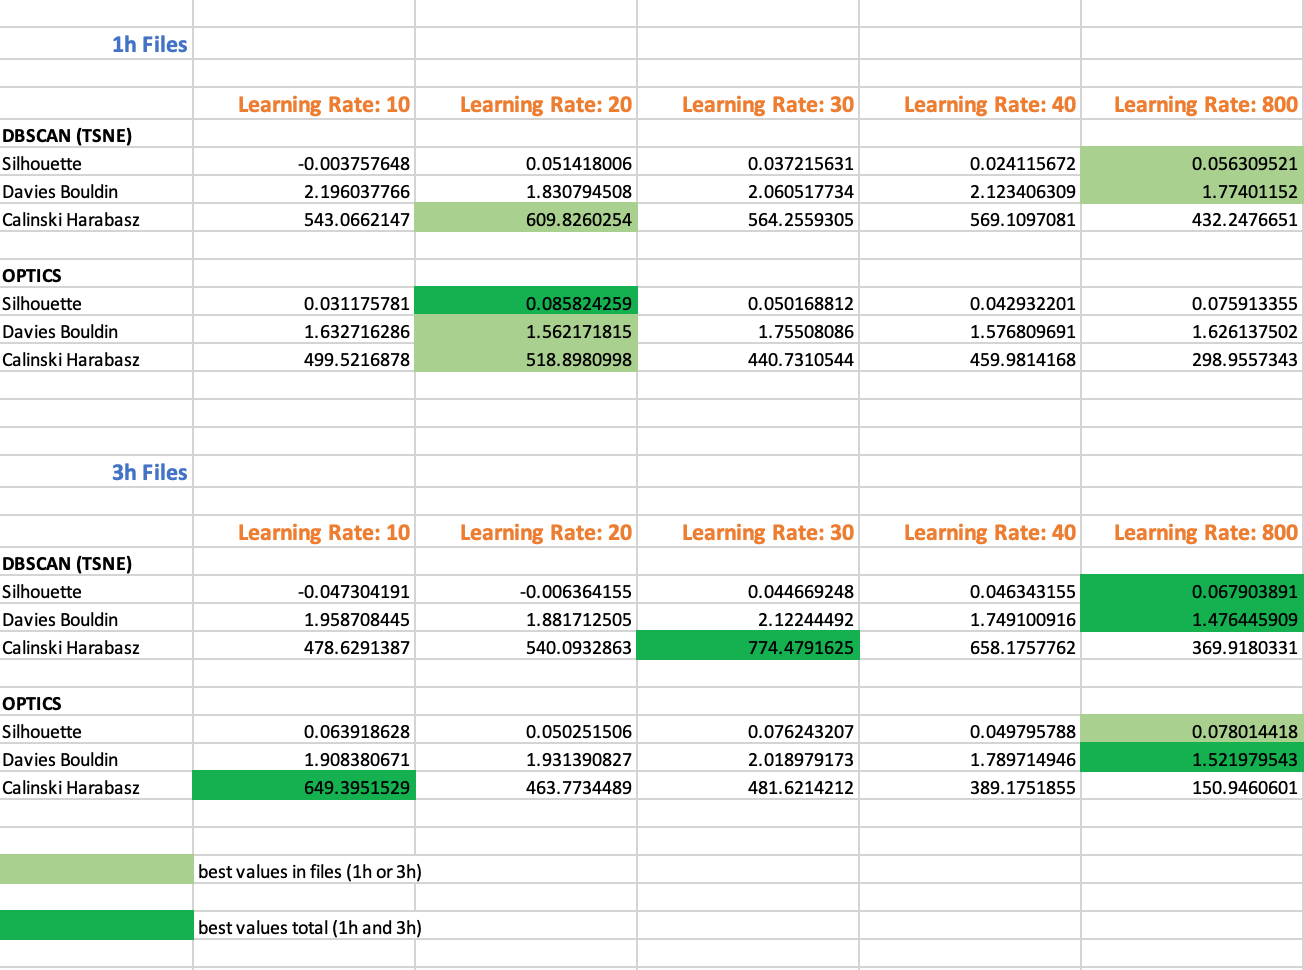
\includegraphics[width=0.8\textwidth]{./images/tsneParametersTest/learningRate/learningRateEvaluationScoresAverageDetailed2.png}
  \caption{Comparison of Silhouette Coefficient, Davies-Bouldin Index, and Caliński-Harabasz Index for different t-SNE \textbf{learning rate} values. Smaller learning rate value steps were taken (i.e. 10, except for the last step to 800) between each test. The lighter green highlighted values indicate the best values of that file aggregation (1h or 3h files). The dark green highlighted values illustrate the overall best values over all files (1h and 3h files).}
  \label{figure:learningRateEvaluationScoresAverageDetailed2}
\end{figure}

\begin{figure}[H]
  \centering
  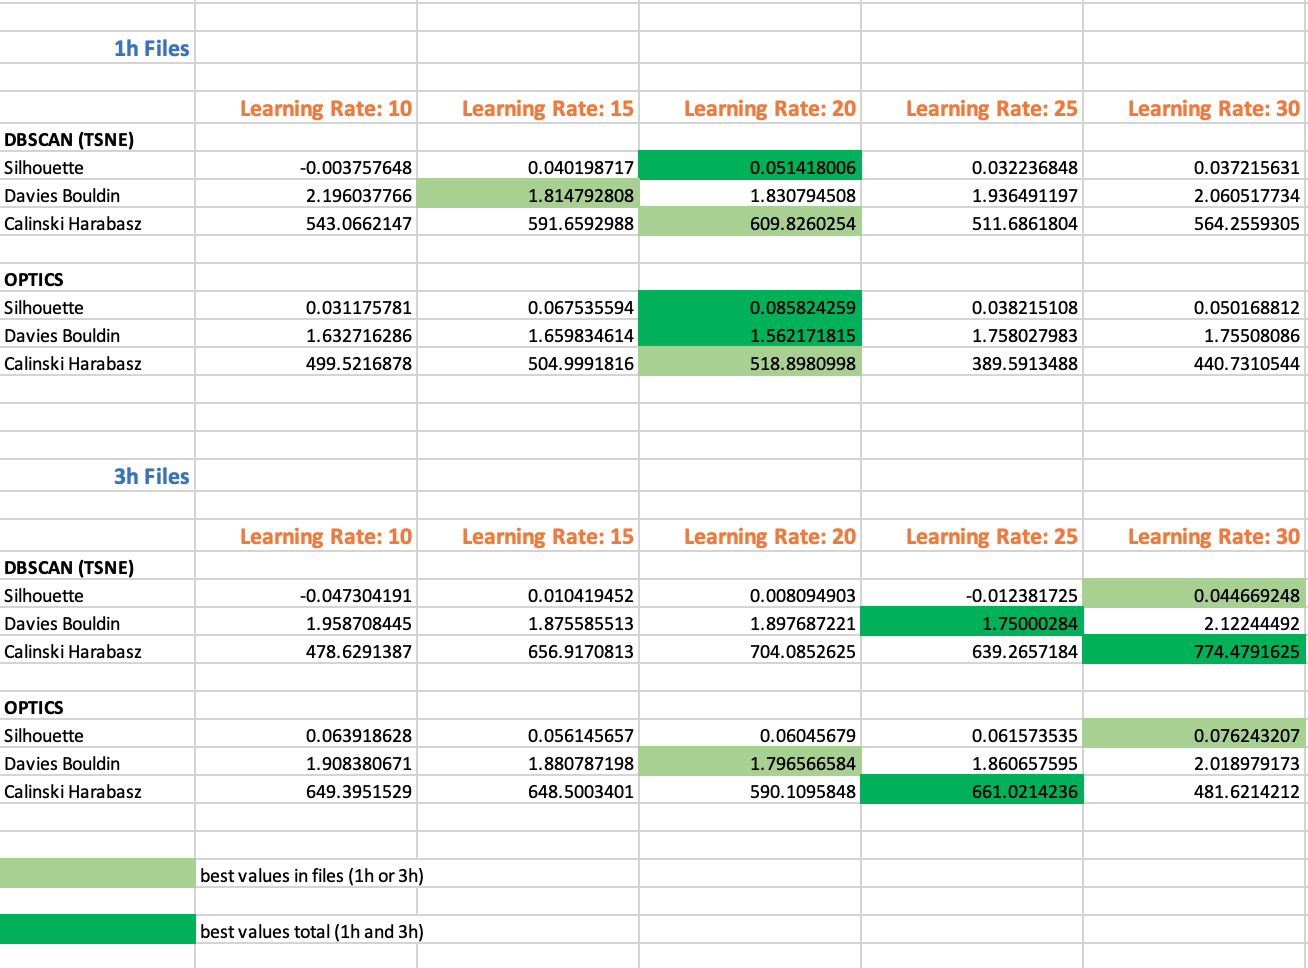
\includegraphics[width=0.8\textwidth]{./images/tsneParametersTest/learningRate/learningRateEvaluationScoresAverageDetailed3.png}
  \caption{Comparison of Silhouette Coefficient, Davies-Bouldin Index, and Caliński-Harabasz Index for different t-SNE \textbf{learning rate} values, in steps of 5. The lighter green highlighted values indicate the best values of that file aggregation (1h or 3h files). The dark green highlighted values illustrate the overall best values over all files (1h and 3h files).}
  \label{figure:learningRateEvaluationScoresAverageDetailed3}
\end{figure}






\subsubsection{Learning Rate Comparison of 20 and 800}
\label{appendig:compareLearningRate20and800}

\begin{figure}[H]
  \centering
  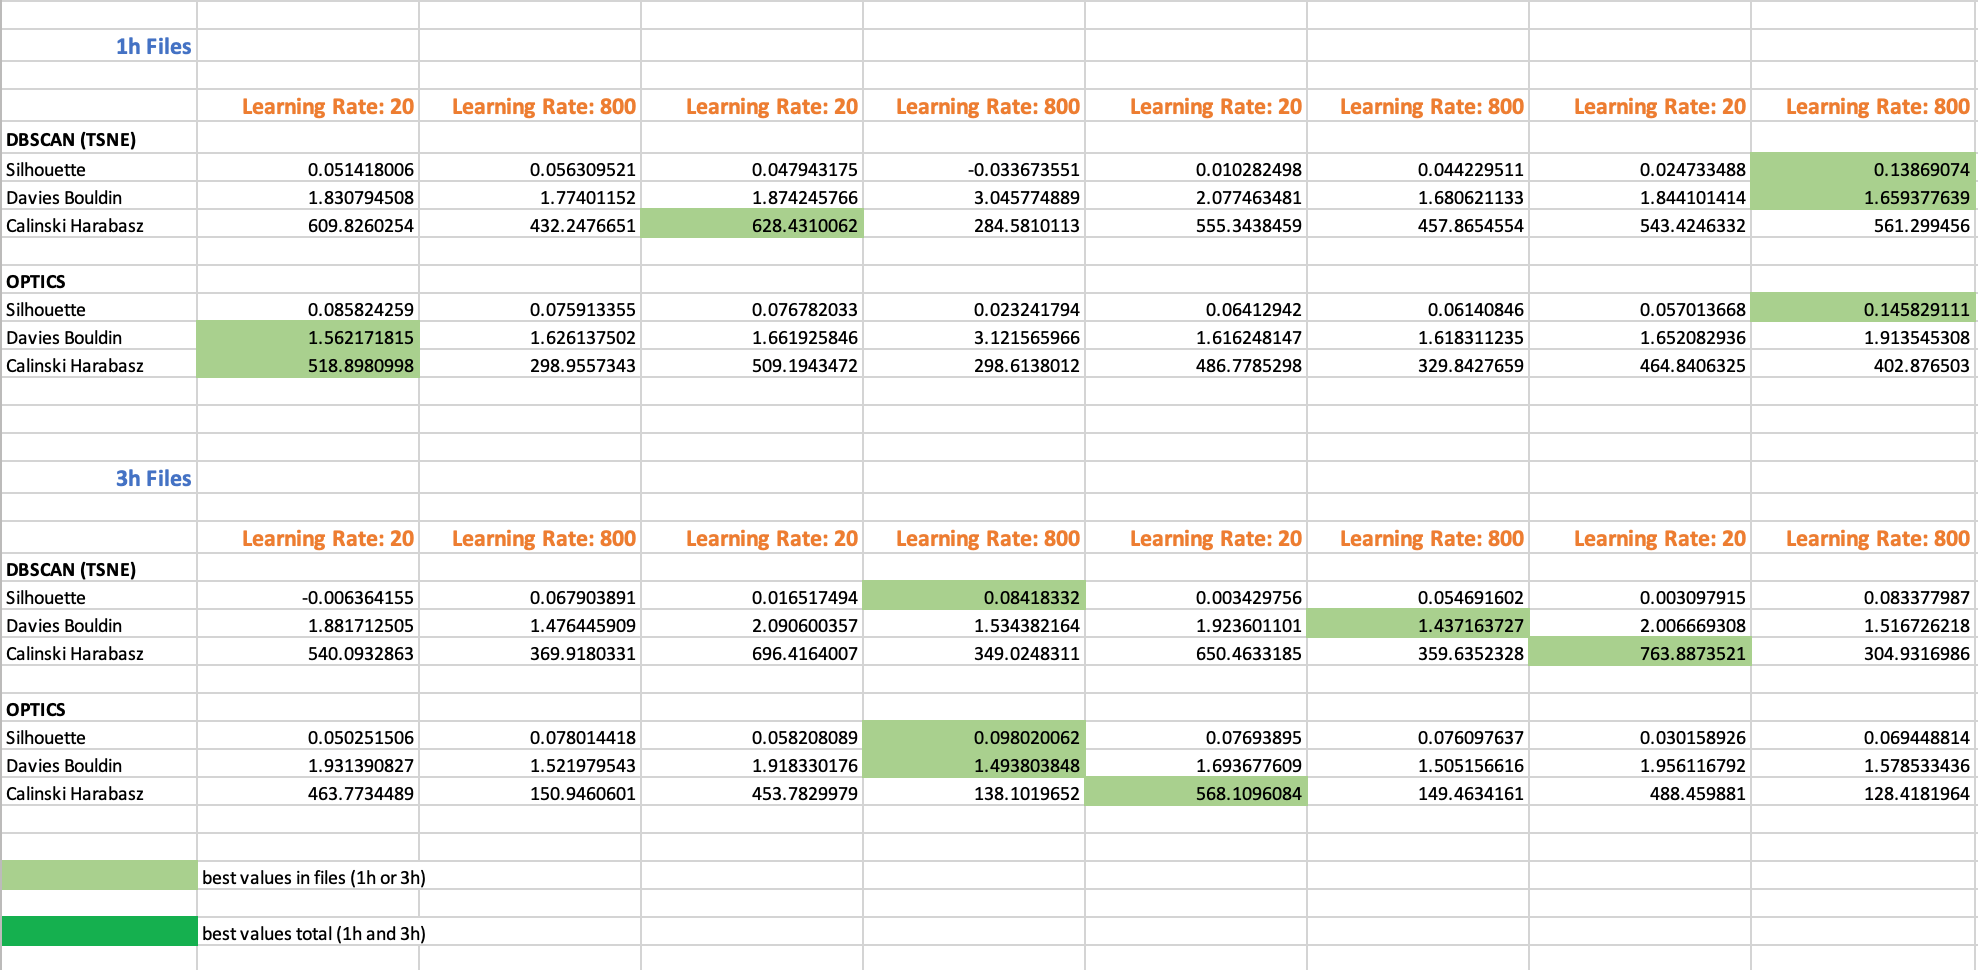
\includegraphics[width=1\textwidth]{./images/tsneParametersTest/learningRate/learningRateEvaluationScoresAverageDetailed4.png}
  \caption{Comparison of Silhouette Coefficient, Davies-Bouldin Index, and Caliński-Harabasz Index for the t-SNE \textbf{learning rate} values 20 and 80. The lighter green highlighted values indicate the best values of that file aggregation (1h or 3h files). The dark green highlighted values illustrate the overall best values over all files (1h and 3h files).}
  \label{figure:learningRateEvaluationScoresAverageDetailed4}
\end{figure}

%------------------ 1h: ------------------
\begin{figure}[H]
  \centering
  \begin{subfigure}{.5\textwidth}
    \centering
    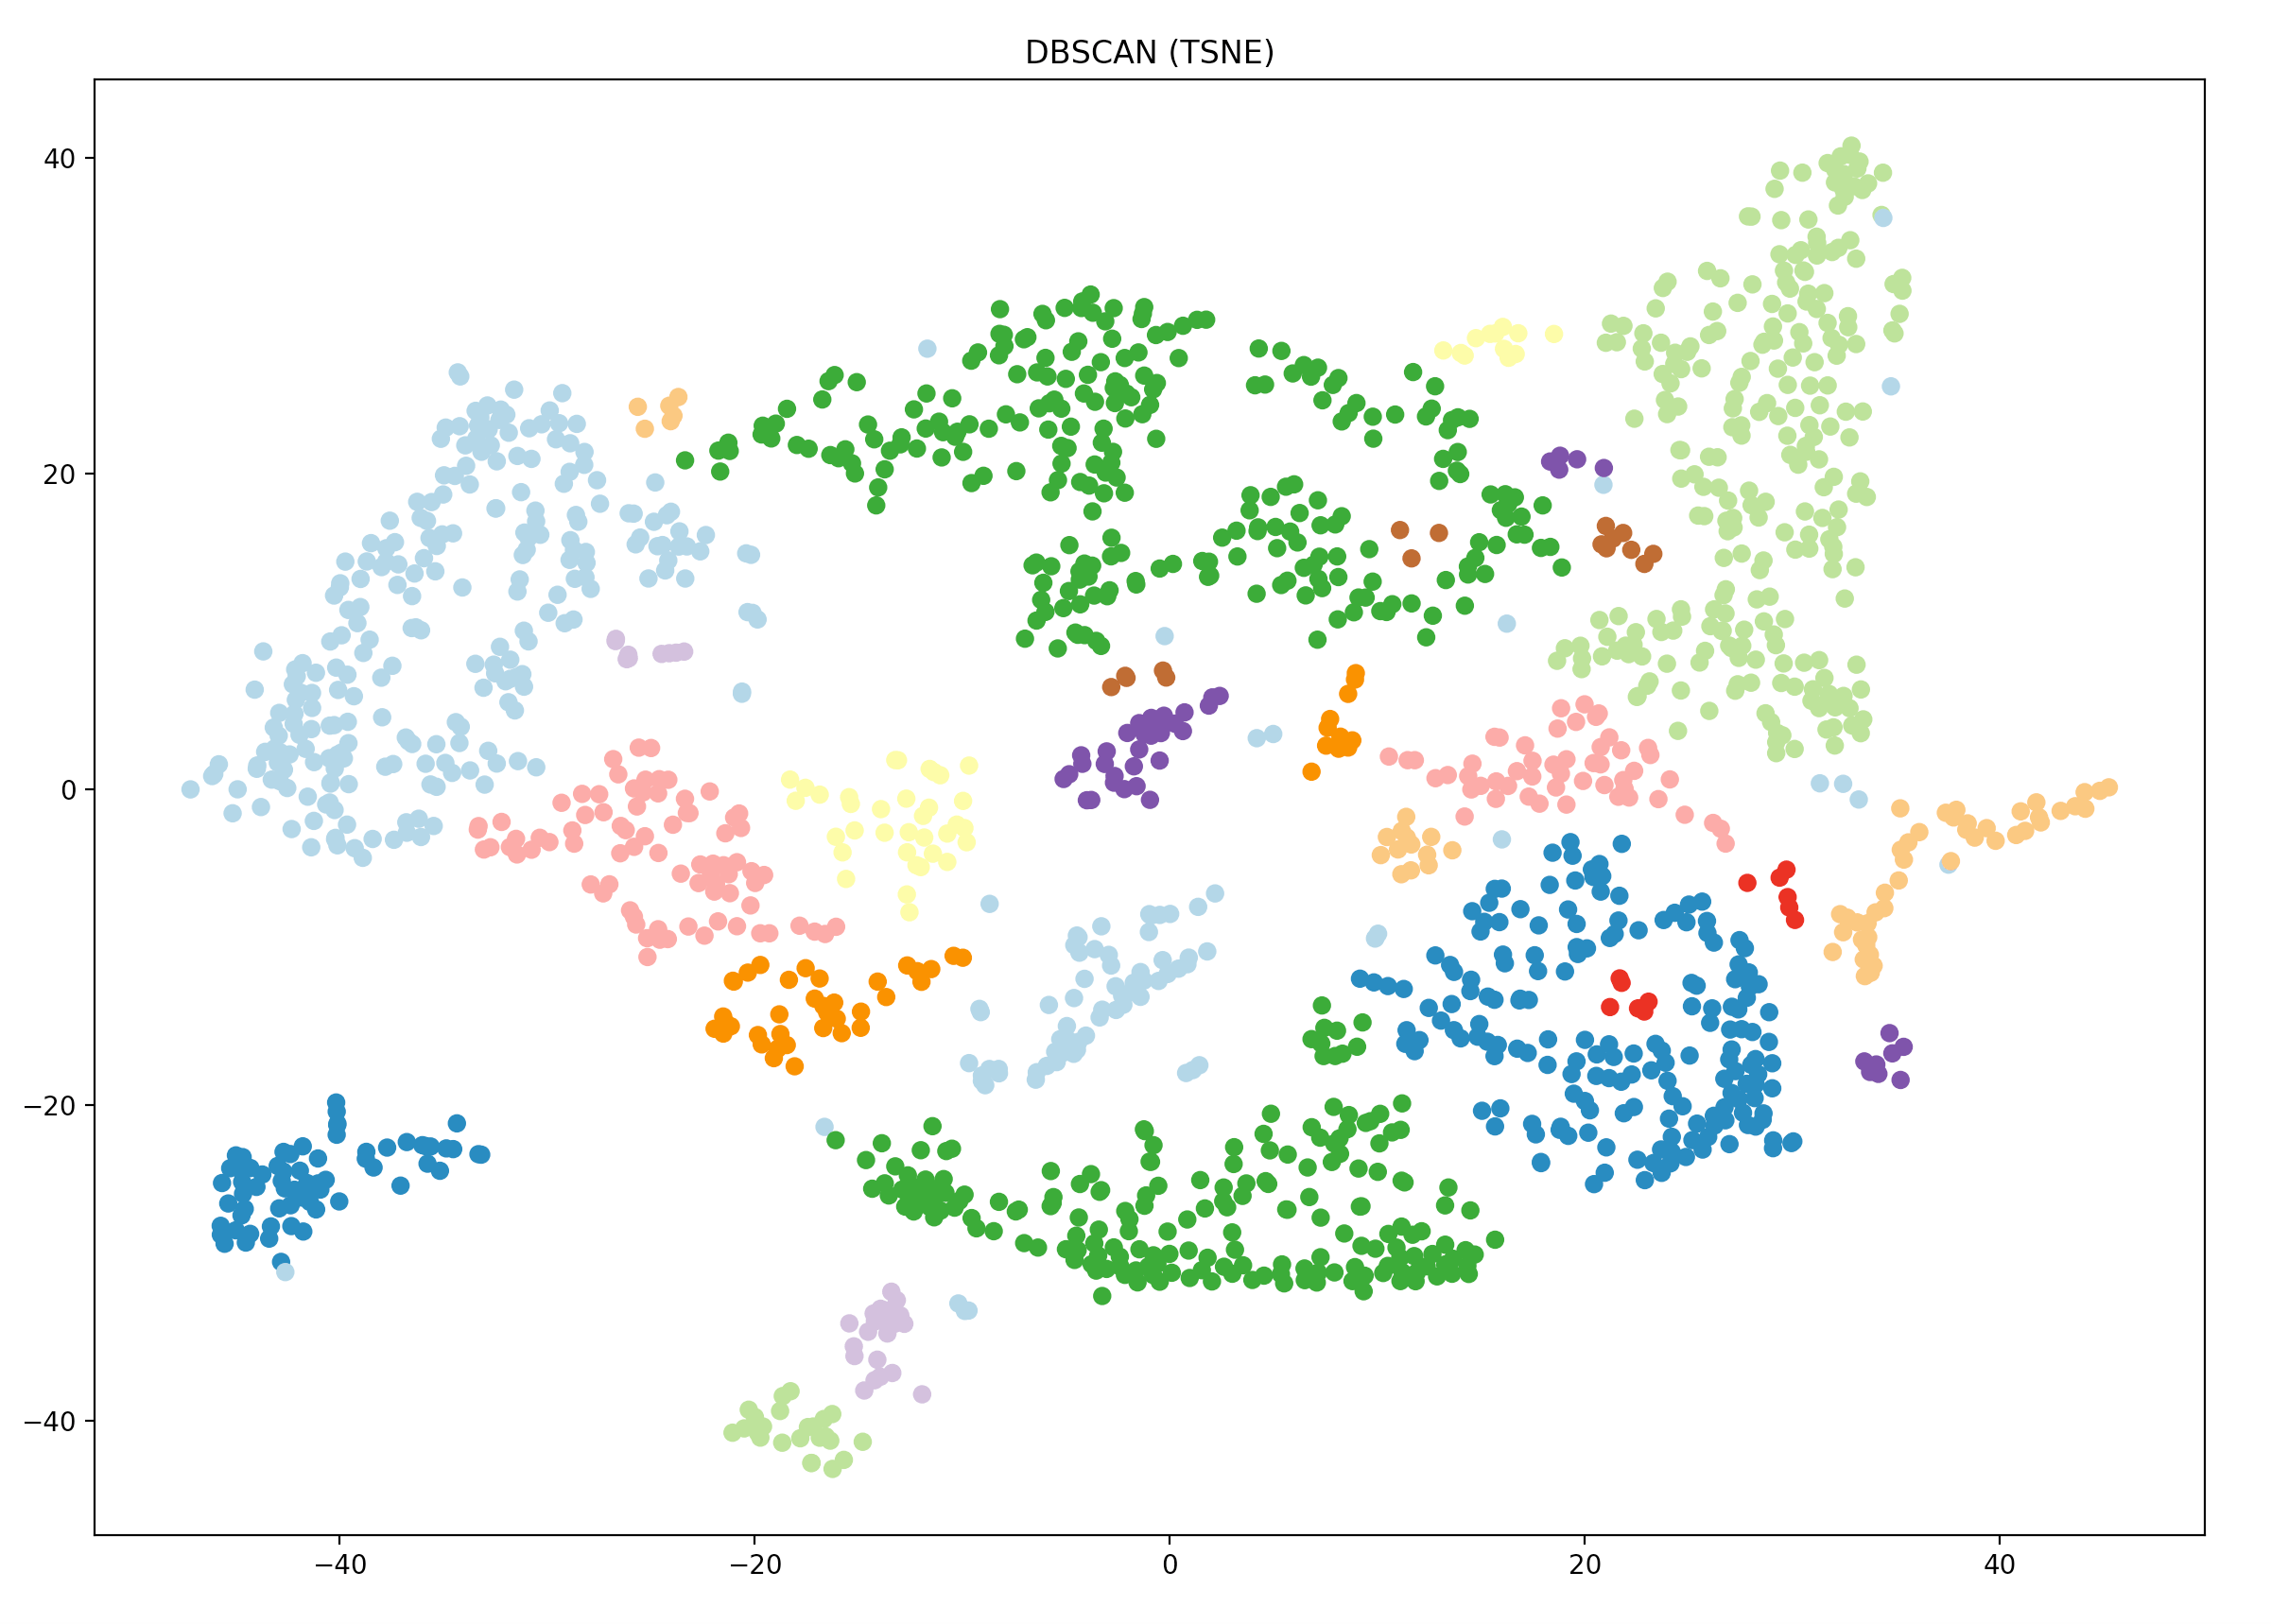
\includegraphics[width=0.9\textwidth]{./images/tsneParametersTest/learningRate/lr201h-DBSCANCompare.png}
  \end{subfigure}%
  \begin{subfigure}{.5\textwidth}
    \centering
    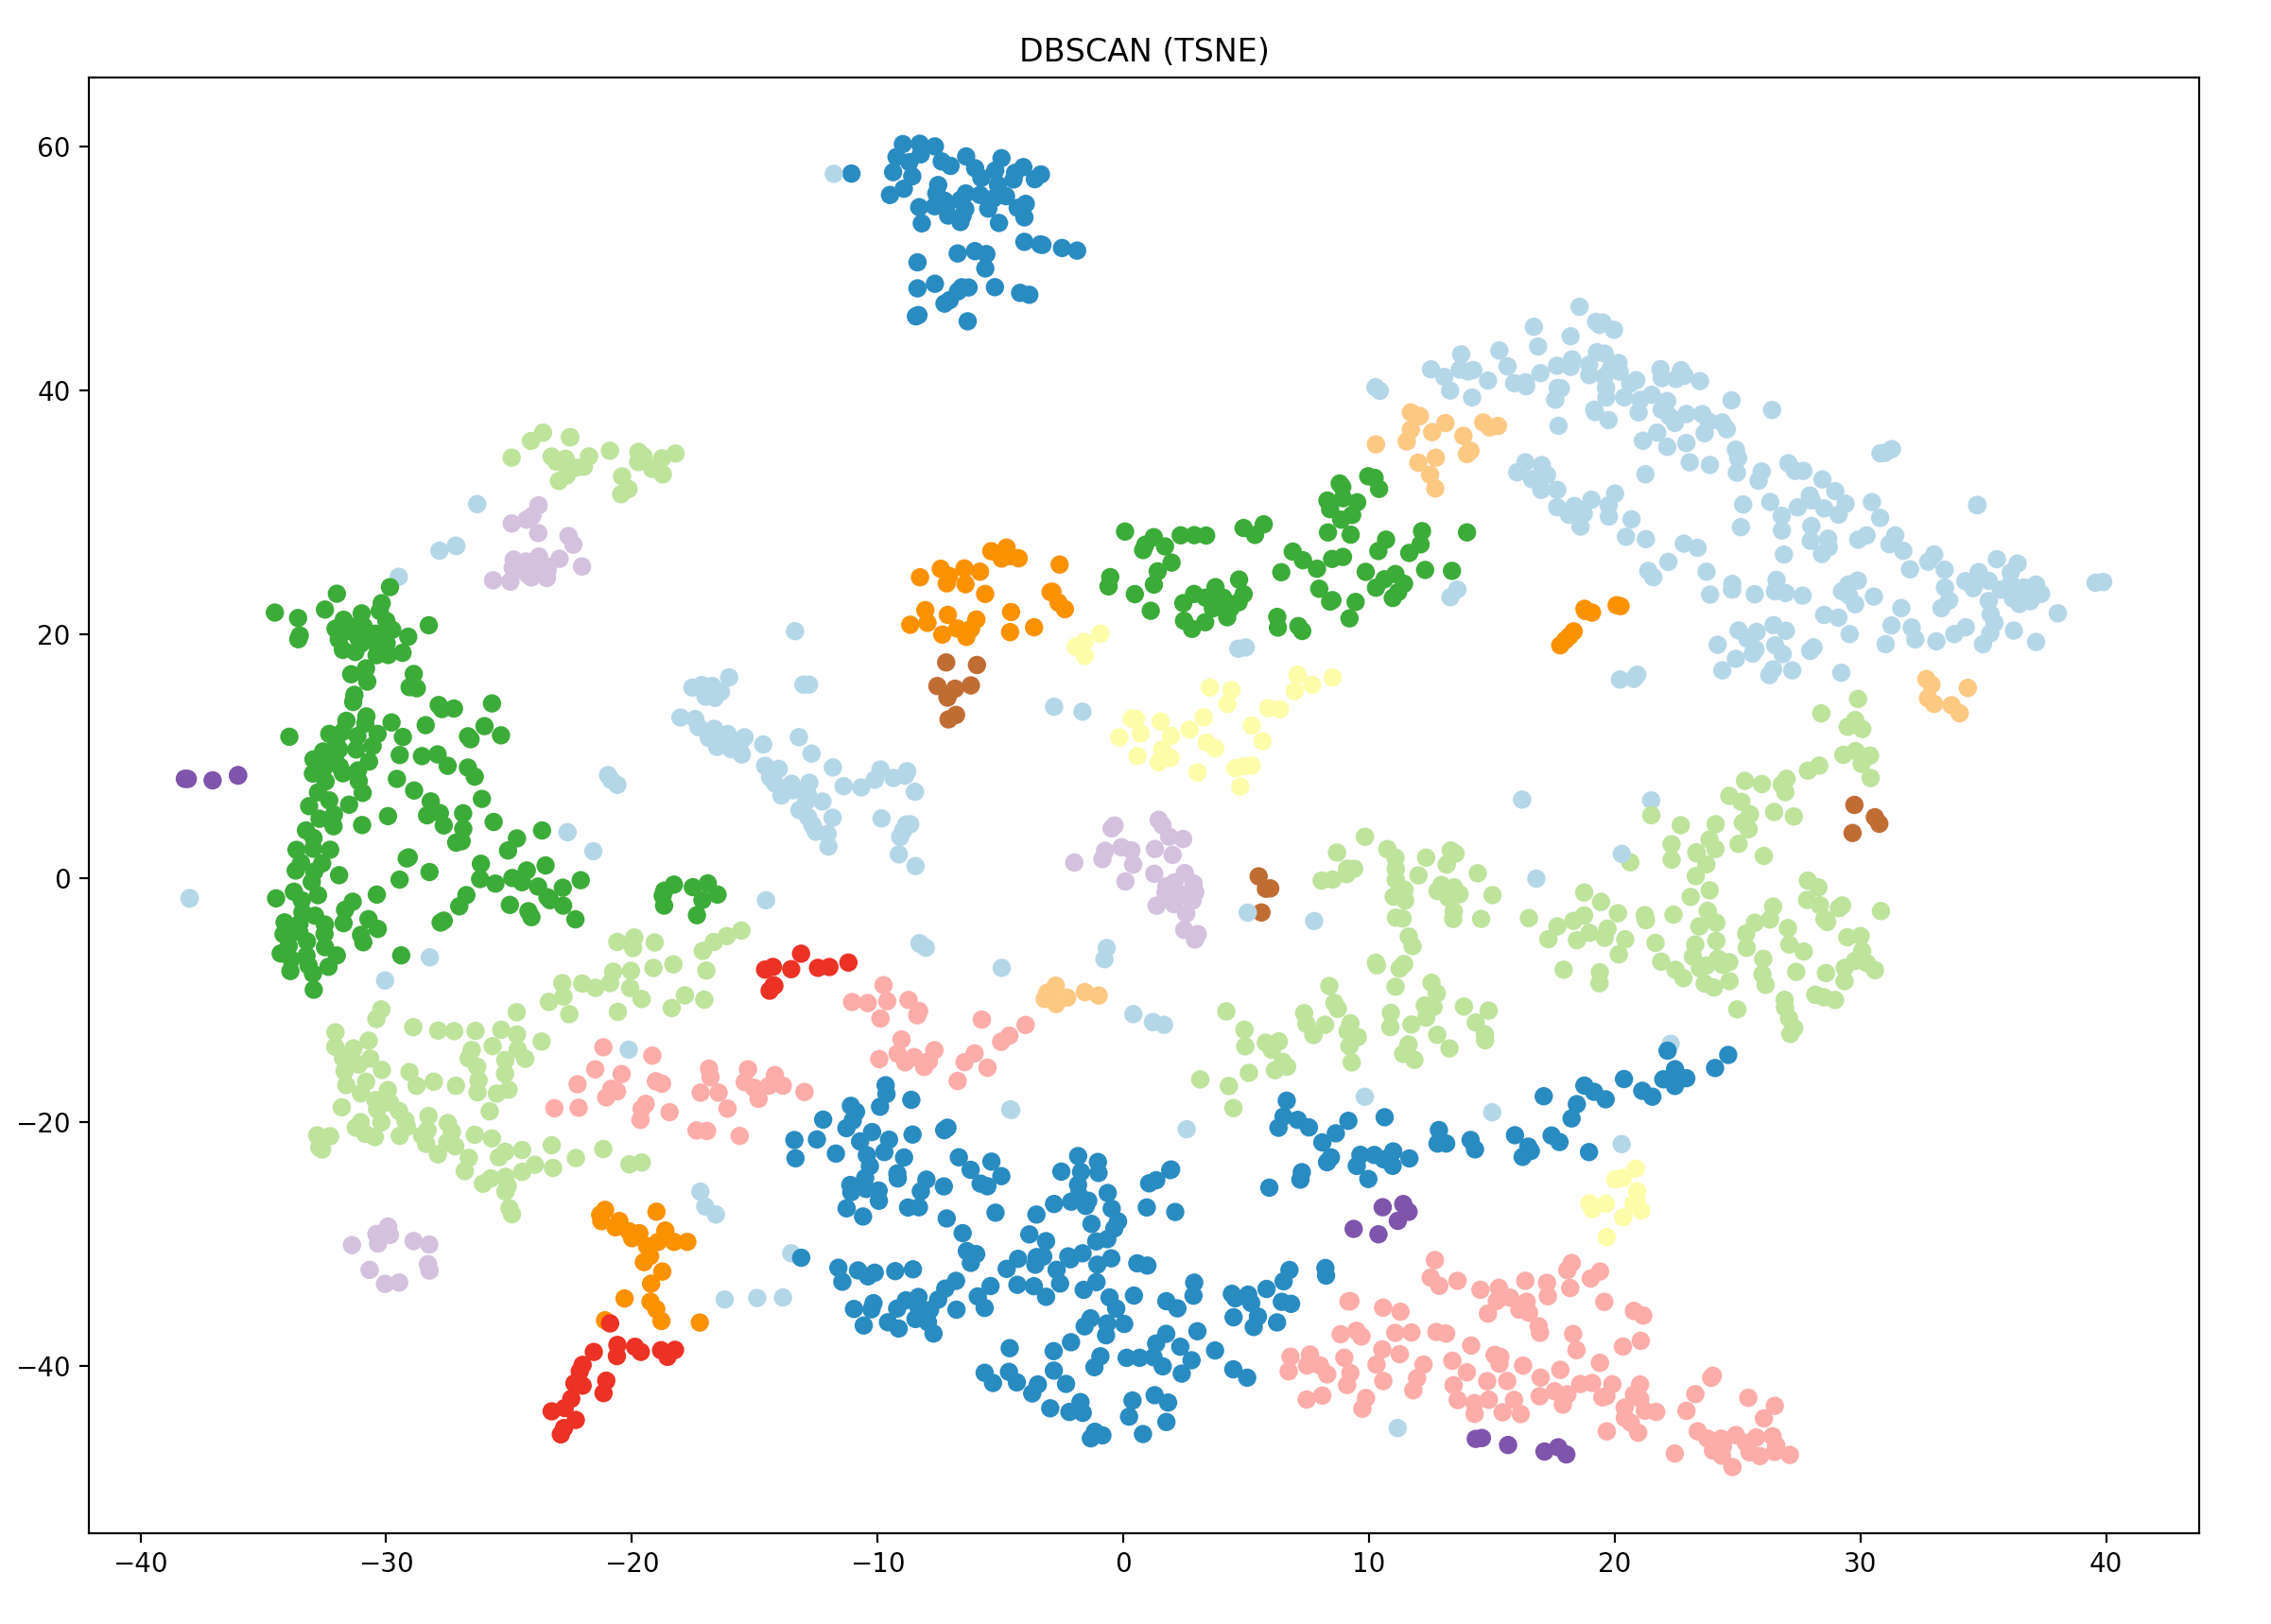
\includegraphics[width=0.9\textwidth]{./images/tsneParametersTest/learningRate/lr8001h-DBSCANCompare.png}
  \end{subfigure}
	\caption{\textbf{1h} data files comparison of learning rate: a) 20, b) 800}
	\label{figure:1h-learningRateComparison20and800}
\end{figure}
%------------------ 3h: ------------------
\begin{figure}[H]
  \centering
  \begin{subfigure}{.5\textwidth}
    \centering
    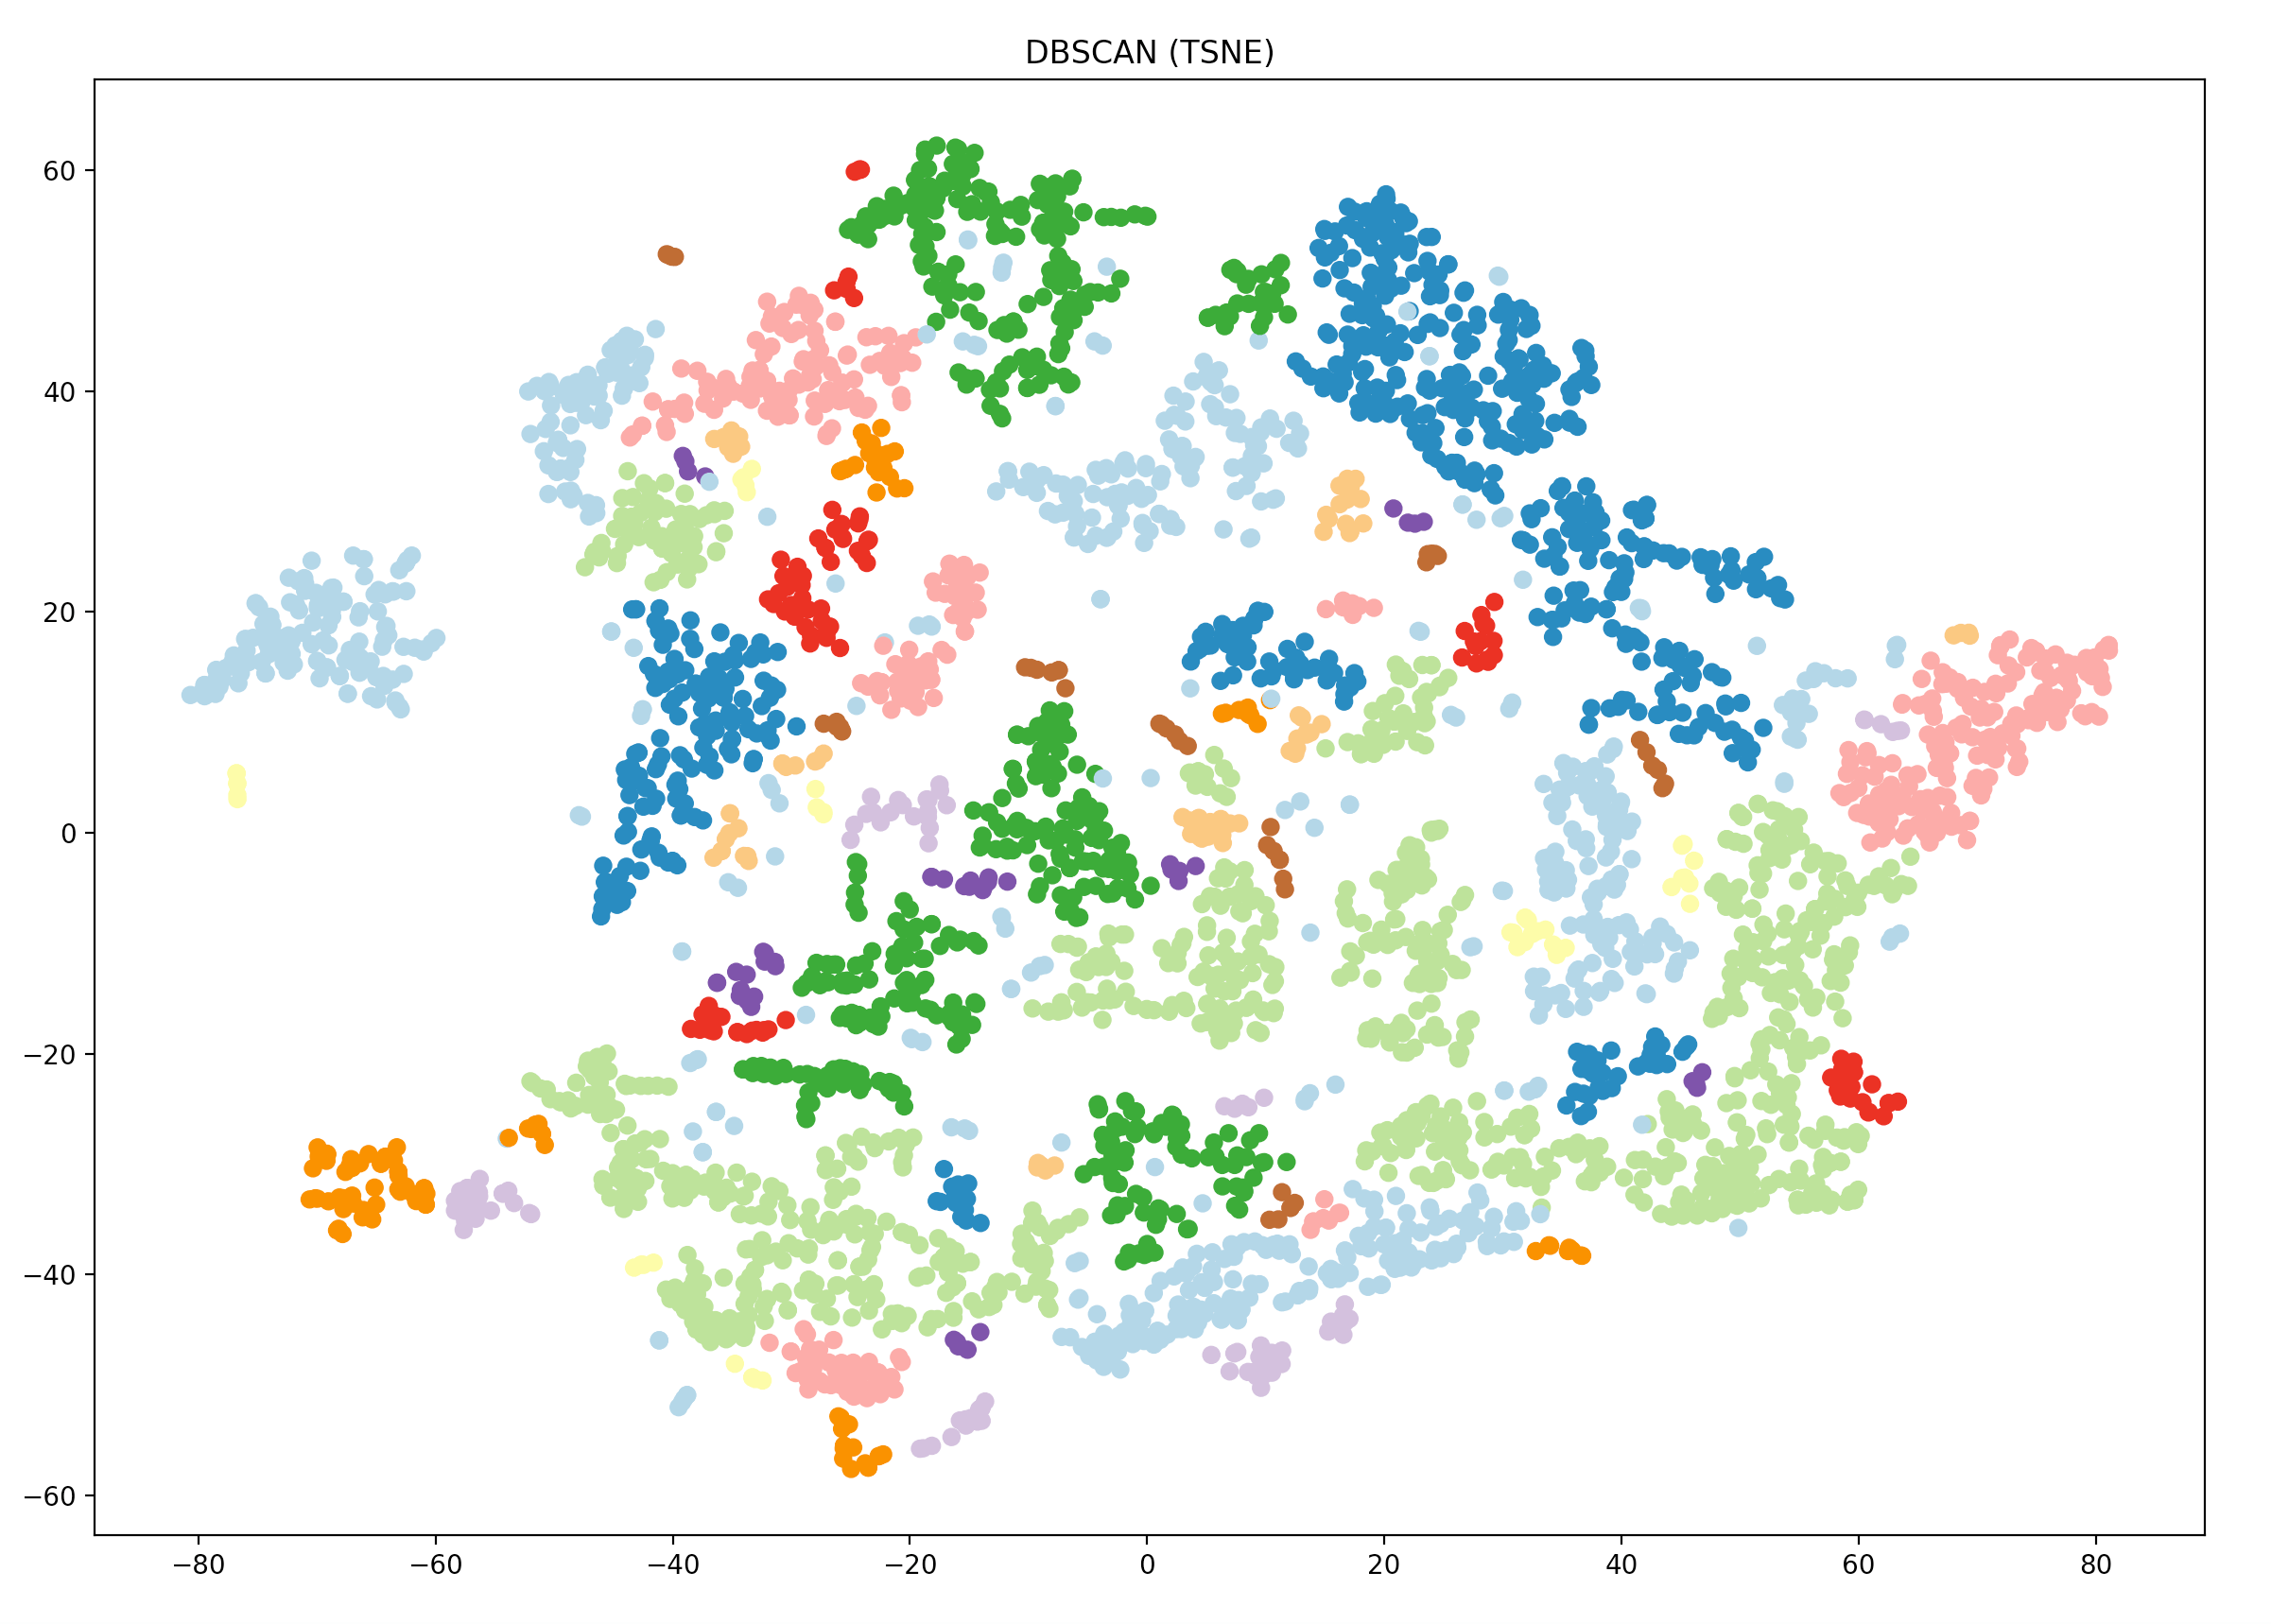
\includegraphics[width=0.9\textwidth]{./images/tsneParametersTest/learningRate/lr203h-DBSCANCompare.png}
  \end{subfigure}%
  \begin{subfigure}{.5\textwidth}
    \centering
    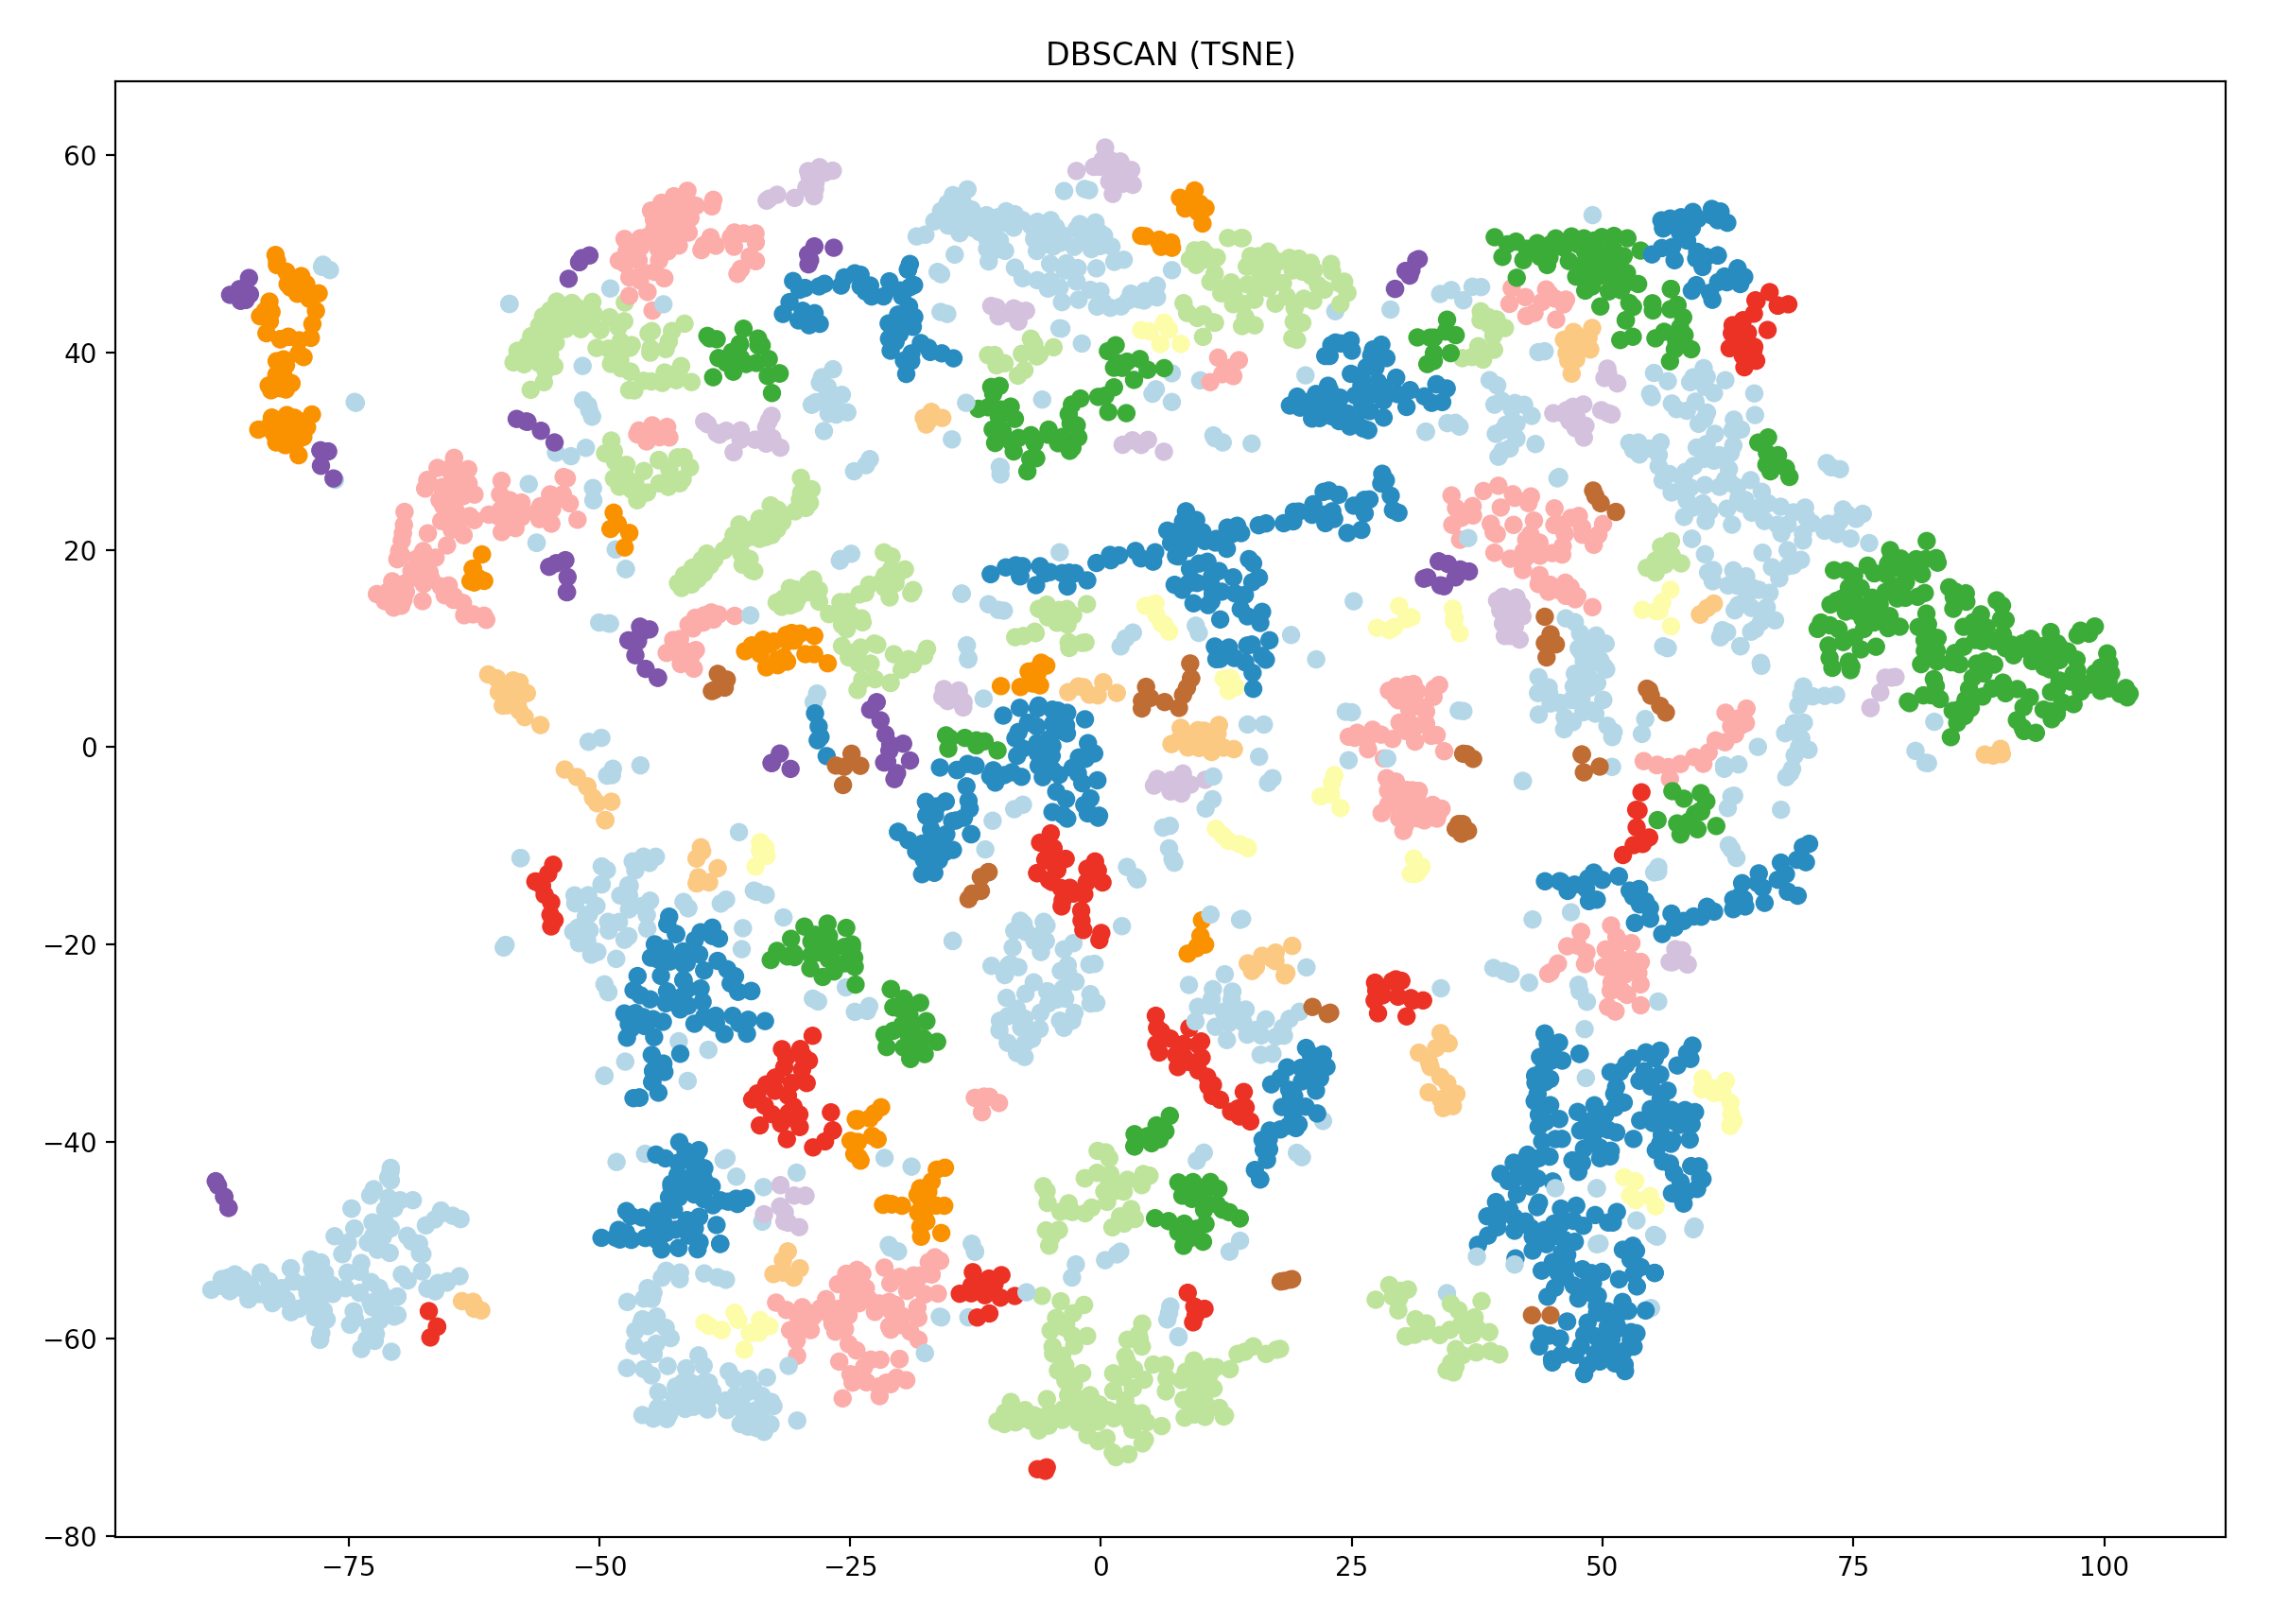
\includegraphics[width=0.9\textwidth]{./images/tsneParametersTest/learningRate/lr8003h-DBSCANCompare.png}
  \end{subfigure}
	\caption{\textbf{3h} data files comparison of learning rate: a) 20, b) 800}
	\label{figure:3h-learningRateComparison20and800}
\end{figure}


\clearpage